% =============================================================================
%
%   PROFESSIONAL PFE THESIS TEMPLATE
%   ──────────────────────────────────
%   Architecture: Modular LaTeX Report
%   Target: VS Code + LaTeX Workshop + TeX Live / MiKTeX
%
% =============================================================================

\documentclass[12pt,a4paper]{report}

% --- Load Packages ---
% =============================================================================
% PACKAGES — Professional PFE Thesis Template
% =============================================================================

% --- Encoding & Language ---
\usepackage[utf8]{inputenc}
\usepackage[T1]{fontenc}
\usepackage{kotex}
\usepackage[french,english]{babel}
\usepackage{csquotes}
\usepackage{ragged2e}

% --- Mathematics ---
\usepackage{amsmath}
\usepackage{amssymb}
\usepackage{calc}

% --- Page Layout ---
\usepackage[
  top=2.5cm,
  bottom=2.5cm,
  left=2.5cm,
  right=2.5cm,
  headheight=15pt
]{geometry}
\usepackage{setspace}

% --- Graphics & Figures ---
\usepackage{graphicx}
\usepackage[font=small,labelfont=bf,labelsep=period]{caption}
\usepackage{subcaption}
\usepackage{float}

% --- Tables ---
\usepackage{booktabs}
\usepackage{array}
\usepackage{longtable}
\usepackage{multirow}
\usepackage{tabularx}

% --- Headers & Footers ---
\usepackage{fancyhdr}

% --- Section Formatting ---
\usepackage{titlesec}

% --- Typography Micro-Adjustments ---
\usepackage{microtype}
\usepackage{mathptmx}
\usepackage{letterspace}

% --- Table of Contents Extras ---
\usepackage[nottoc,notlof,notlot]{tocbibind}

% --- Colors ---
\usepackage[dvipsnames,svgnames,table]{xcolor}

% --- Lists ---
\usepackage{enumitem}

% --- TikZ & Boxes ---
\usepackage{tikz}
\usetikzlibrary{calc}
\usepackage[most]{tcolorbox}

% --- Bibliography ---
\usepackage[
  backend=biber,
  style=numeric,
  sorting=nyt,
  maxbibnames=99
]{biblatex}

% --- Hyperlinks (load late) ---
\usepackage[
  colorlinks=true,
  linkcolor=NavyBlue,
  citecolor=ForestGreen,
  urlcolor=RoyalBlue,
  bookmarks=true,
  bookmarksopen=true,
  pdfstartview=FitH
]{hyperref}

% --- Smart References (load after hyperref) ---
\usepackage[capitalise,noabbrev]{cleveref}


% --- Load Settings ---
% =============================================================================
% SETTINGS — Professional PFE Thesis Template
% =============================================================================

% --- Bibliography Resource ---
\addbibresource{bibliography/references.bib}

% --- Graphics Path ---
\graphicspath{{figures/}}

% --- Line Spacing ---
\onehalfspacing

% --- Paragraph Settings ---
\setlength{\parindent}{1.25cm}
\setlength{\parskip}{6pt plus 2pt minus 1pt}

% --- Numbering Depth ---
\setcounter{secnumdepth}{3}

% --- Header & Footer Style ---
\pagestyle{fancy}
\fancyhf{}
\fancyhead[L]{\nouppercase{\leftmark}}
\fancyhead[R]{\thepage}
\renewcommand{\headrulewidth}{0.4pt}
\renewcommand{\footrulewidth}{0pt}

\fancypagestyle{plain}{%
  \fancyhf{}
  \fancyfoot[C]{\thepage}
  \renewcommand{\headrulewidth}{0pt}
  \renewcommand{\footrulewidth}{0pt}
}

% --- Section Formatting ---
\titleformat{\section}
  {\normalfont\Large\bfseries\color{MidnightBlue!90}}
  {\thesection}
  {1em}
  {}
\titlespacing*{\section}{0pt}{3.5ex plus 1ex minus .2ex}{2.3ex plus .2ex}

% --- Subsection Formatting ---
\titleformat{\subsection}
  {\normalfont\large\bfseries\color{MidnightBlue!80}}
  {\thesubsection}
  {1em}
  {}
\titlespacing*{\subsection}{0pt}{3.25ex plus 1ex minus .2ex}{1.5ex plus .2ex}

% --- Subsubsection Formatting ---
\titleformat{\subsubsection}
  {\normalfont\normalsize\bfseries\color{MidnightBlue!70}}
  {\thesubsubsection}
  {1em}
  {}

% --- Float Placement ---
\renewcommand{\topfraction}{0.9}
\renewcommand{\bottomfraction}{0.8}
\renewcommand{\textfraction}{0.1}
\renewcommand{\floatpagefraction}{0.8}

% --- PDF Metadata ---
\hypersetup{
  pdftitle={Projet de Fin d'Études},
  pdfauthor={Author Name},
  pdfsubject={PFE Thesis},
  pdfkeywords={PFE, Thesis, Startup, Lean Canvas, Business Model Canvas}
}


% --- Load Custom Commands ---
% =============================================================================
% CUSTOM COMMANDS — Professional PFE Thesis Template
% =============================================================================

% --- Cross-Reference Shortcuts ---
\newcommand{\figref}[1]{\cref{fig:#1}}
\newcommand{\tabref}[1]{\cref{tab:#1}}
\newcommand{\chapref}[1]{\cref{chap:#1}}
\newcommand{\secref}[1]{\cref{sec:#1}}
\newcommand{\appref}[1]{\cref{app:#1}}

% --- Text Shortcuts ---
\newcommand{\ie}{\textit{i.e.}\xspace}
\newcommand{\eg}{\textit{e.g.}\xspace}
\newcommand{\etal}{\textit{et al.}\xspace}

% --- Highlight Box ---
\newtcolorbox{highlightbox}[1][]{%
  colback=MidnightBlue!5,
  colframe=MidnightBlue!60,
  fonttitle=\bfseries,
  title={#1},
  arc=2mm,
  boxrule=0.8pt,
  left=8pt,
  right=8pt,
  top=6pt,
  bottom=6pt
}

% --- Definition Box ---
\newtcolorbox{definitionbox}[1][]{%
  colback=ForestGreen!5,
  colframe=ForestGreen!60,
  fonttitle=\bfseries,
  title={#1},
  arc=2mm,
  boxrule=0.8pt,
  left=8pt,
  right=8pt,
  top=6pt,
  bottom=6pt
}

% --- Warning / Important Box ---
\newtcolorbox{importantbox}[1][]{%
  colback=BrickRed!5,
  colframe=BrickRed!60,
  fonttitle=\bfseries,
  title={#1},
  arc=2mm,
  boxrule=0.8pt,
  left=8pt,
  right=8pt,
  top=6pt,
  bottom=6pt
}

% =============================================================================
% BUSINESS MODEL CANVAS ENVIRONMENT
% =============================================================================
\definecolor{bmcblue}{HTML}{3498DB}
\definecolor{bmcgreen}{HTML}{2ECC71}
\definecolor{bmcorange}{HTML}{E67E22}
\definecolor{bmcred}{HTML}{E74C3C}
\definecolor{bmcpurple}{HTML}{9B59B6}
\definecolor{bmcgray}{HTML}{95A5A6}

\newtcolorbox{bmcblock}[2][]{%
  colback=#2!8,
  colframe=#2!70,
  fonttitle=\bfseries\small,
  title={#1},
  arc=1.5mm,
  boxrule=0.6pt,
  left=5pt,
  right=5pt,
  top=4pt,
  bottom=4pt,
  fontupper=\small
}

% --- BMC Section Command ---
\newcommand{\bmcsection}[3]{%
  \begin{bmcblock}[#1]{#2}
    #3
  \end{bmcblock}
  \vspace{4pt}
}

% =============================================================================
% LEAN CANVAS ENVIRONMENT
% =============================================================================
\definecolor{leanpink}{HTML}{E91E63}
\definecolor{leanteal}{HTML}{009688}
\definecolor{leanamber}{HTML}{FF9800}

\newtcolorbox{leanblock}[2][]{%
  colback=#2!8,
  colframe=#2!70,
  fonttitle=\bfseries\small,
  title={#1},
  arc=1.5mm,
  boxrule=0.6pt,
  left=5pt,
  right=5pt,
  top=4pt,
  bottom=4pt,
  fontupper=\small
}

\newcommand{\leansection}[3]{%
  \begin{leanblock}[#1]{#2}
    #3
  \end{leanblock}
  \vspace{4pt}
}

% =============================================================================
% SPRINT TABLE COMMAND
% =============================================================================
\newcommand{\sprinttable}[5]{%
  % #1 = Sprint number
  % #2 = Duration
  % #3 = Goal
  % #4 = User stories (tabular content rows)
  % #5 = Deliverables
  \begin{table}[H]
    \centering
    \caption{Sprint #1 — #3}
    \label{tab:sprint-#1}
    \begin{tabularx}{\textwidth}{l X}
      \toprule
      \textbf{Sprint}       & #1 \\
      \textbf{Duration}     & #2 \\
      \textbf{Goal}         & #3 \\
      \midrule
      \textbf{User Stories} & #4 \\
      \midrule
      \textbf{Deliverables} & #5 \\
      \bottomrule
    \end{tabularx}
  \end{table}
}

% =============================================================================
% METRICS DASHBOARD PLACEHOLDER
% =============================================================================
\newcommand{\metriccard}[2]{%
  \begin{tcolorbox}[
    colback=bmcblue!5,
    colframe=bmcblue!50,
    width=0.48\textwidth,
    arc=2mm,
    boxrule=0.5pt,
    halign=center
  ]
    \textbf{#1}\\[4pt]
    {\Large\bfseries\color{MidnightBlue} #2}
  \end{tcolorbox}
}

% =============================================================================
% BLACK & WHITE CHAPTER OPENING PAGE — Times New Roman Style
% =============================================================================
% Add to packages.tex:
%   \usepackage{mathptmx}   % Times New Roman for pdfLaTeX
%   \usepackage{lmodern}
%   \usepackage{letterspace} % for letter-spacing (from microtype — already loaded)

\newlength{\chapteropeningnumwidth}
\newlength{\chapiterheight}

\newcommand{\chapteropening}[4]{%
  \clearpage
  \newgeometry{top=2cm, bottom=2cm, left=2.5cm, right=2cm}
  \thispagestyle{empty}%

  % ── 1. Measure width of number at 120pt ───────────────────────────────────
  \settowidth{\chapteropeningnumwidth}{%
    {\fontsize{120}{120}\selectfont\bfseries\rmfamily #1}}%

  % ── 2. Chapter number (120pt, Times, bold) ────────────────────────────────
  \noindent
  {\fontsize{120}{120}\selectfont\bfseries\rmfamily #1\par}%
  \vspace{4pt}%

  % ── 3. CHAPITER — stretched to number width + letter-spacing ──────────────
  \noindent\resizebox{\chapteropeningnumwidth}{!}{%
    {\fontsize{11}{11}\selectfont\bfseries\rmfamily\textls[200]{CHAPITER}}%
  }\par%

  % ── 4. Measure height of CHAPITER label for rule start ────────────────────
  \settototalheight{\chapiterheight}{%
    {\fontsize{11}{11}\selectfont\bfseries\rmfamily CHAPITER}}%

  % ── 5. Spacer — push title to lower half ──────────────────────────────────
  \vspace*{\fill}

  % ── 6. Title (60pt, Times, bold) ──────────────────────────────────────────
  \noindent\hspace{20pt}%
  \begin{minipage}[t]{0.85\textwidth}
    {\fontsize{50}{62}\selectfont\bfseries\rmfamily #2\par}%
  \end{minipage}

  \vspace*{2cm}

  % ── 7. Vertical rule: starts at middle of CHAPITER, ends at title bottom ──
  \begin{tikzpicture}[remember picture, overlay]
    \draw[line width=2pt, black]
      % start: middle of CHAPITER label (top=2cm, number~120pt≈4.2cm, label~0.4cm → middle ≈ 6.4cm)
      ($(current page.north west) + (2.5cm, -6.4cm)$)
      --
      % end: bottom of title block (~4cm from bottom)
      ($(current page.south west) + (2.5cm, 4cm)$);
  \end{tikzpicture}

  \restoregeometry
  \clearpage
  \chapter{#3}
  \label{#4}
}

% =============================================================================
% DOCUMENT BEGIN
% =============================================================================
\begin{document}

% ─────────────────────────────────────────────────────────────────────────────
% FRONT MATTER
% ─────────────────────────────────────────────────────────────────────────────

% --- Cover Page (no visible page number) ---
\thispagestyle{empty}
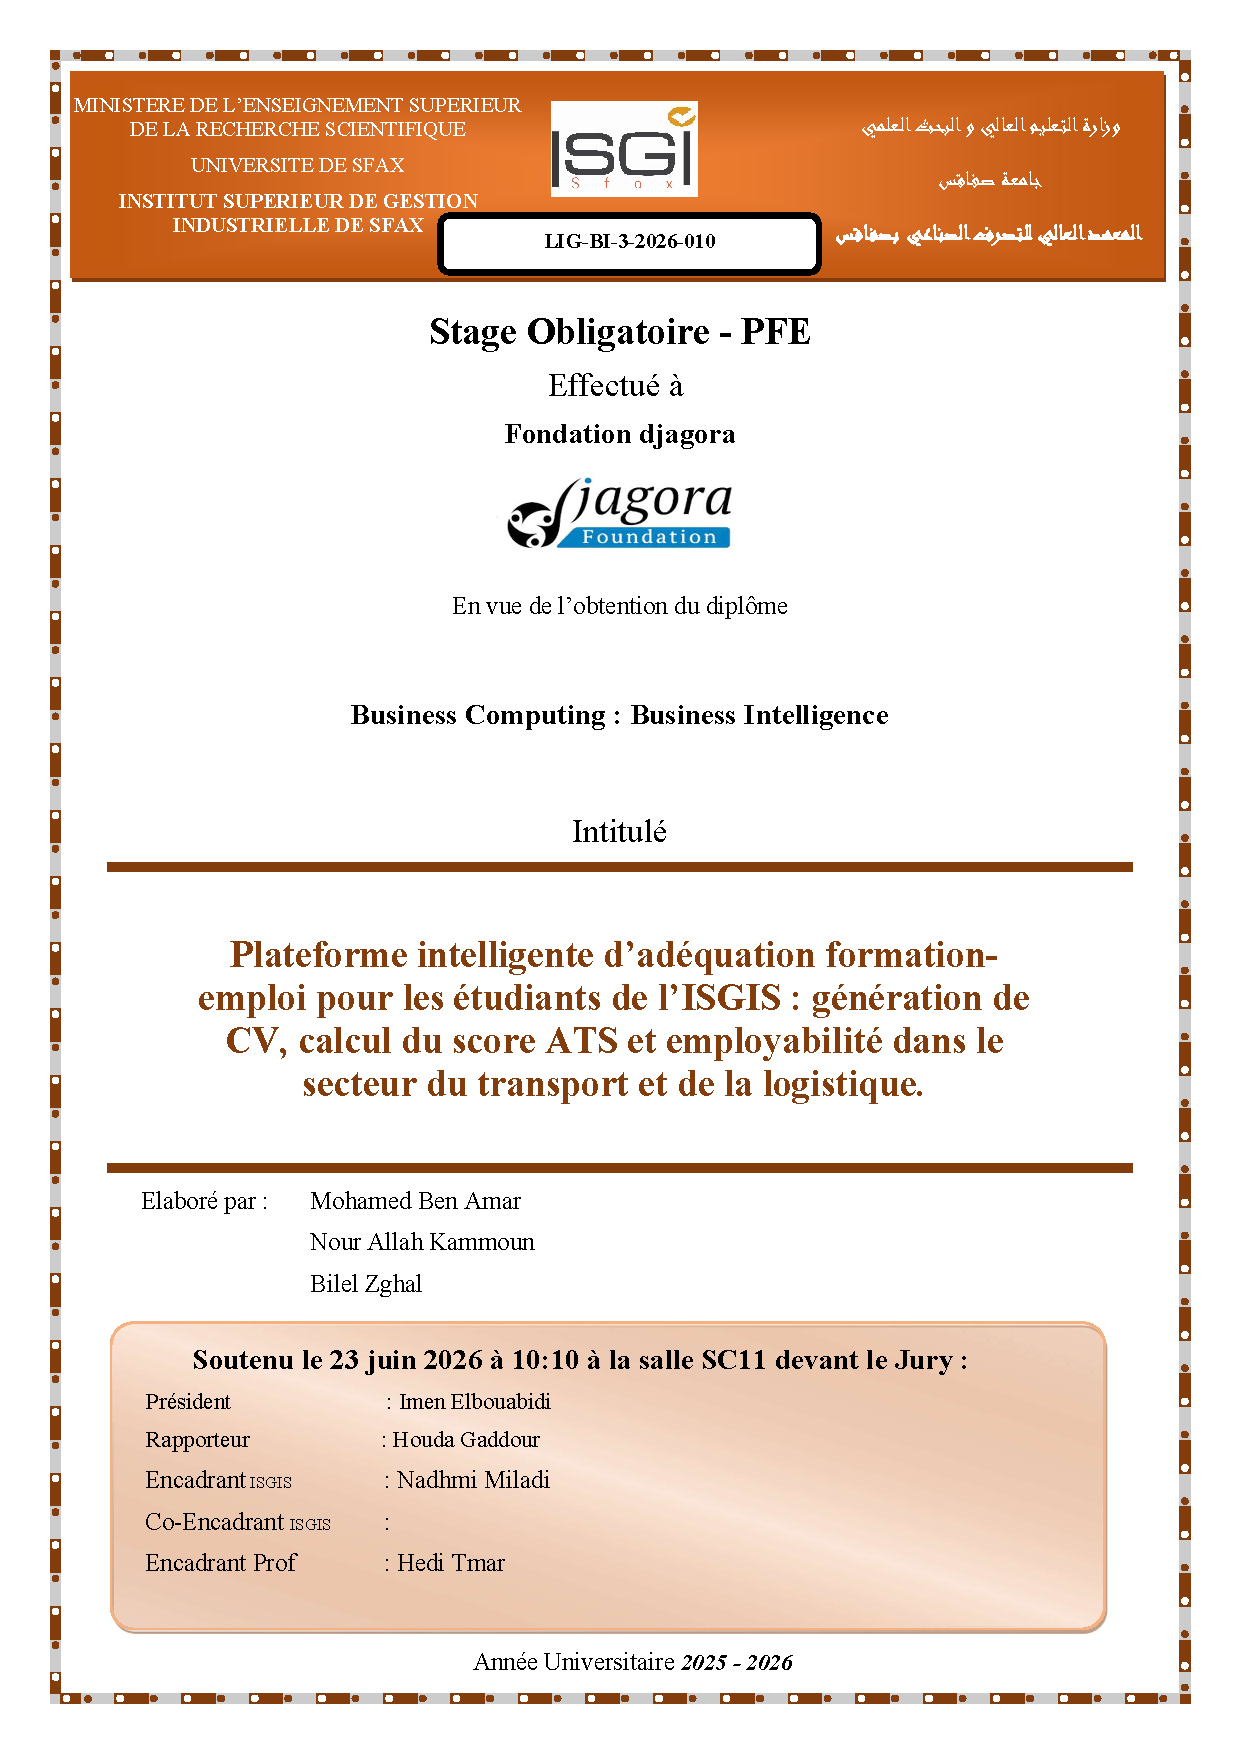
\includepdf[pages=1, pagecommand={}]{final garde.pdf}


% --- Roman numbering starts from dedication ---
\pagenumbering{roman}

% --- Dedication (page i) ---
% =============================================================================
% DEDICATION
% =============================================================================

\chapter*{Dédicaces}
\addcontentsline{toc}{chapter}{Dédicaces}

\vspace{12pt}

\begin{center}
  \begin{minipage}{0.85\textwidth}
    \centering
    \normalsize\itshape

    \textbf{À mon cher père Mohamed},\\

    Je dédie ce travail avec tout mon amour et ma profonde gratitude. Merci pour tes encouragements constants et pour avoir toujours cru en moi. Ta présence et ta confiance m'ont toujours donné la force de continuer et de ne jamais abandonner.\\

    \textbf{À ma tendre mère Sonia},\\

 Je dédie ce travail avec tout mon amour et ma reconnaissance. Je vous remercie pour votre encouragement  constant, vos encouragements et tous les sacrifices que vous avez faits pour moi. Votre présence et votre confiance m’ont toujours donné la force d’avancer et de persévérer.\\

    \textbf{À mes chers frères Alaa et Hassen ,ainsi qu'à leurs chères épouses Rim et Sirine},\\

    J'adresse également mes sincères remerciements pour leur soutien, leurs encouragements et leur bienveillance tout au long de ce parcours.\\

    \textbf{À mes adorables neveux, Edam et Youssef},\\

    Je vous remercie pour votre énergie positive ainsi que pour les moments de bonheur et de rire que vous m'avez offerts.\\

    \textbf{À mes deux binômes Mohamed et Bilel},\\

    Je vous remercie pour cette expérience de travail enrichissante, pour votre professionnalisme, votre sérieux, ainsi que pour votre collaboration et votre esprit d'équipe tout au long de ce projet.\\

    \textbf{À tous mes amis},\\

    Je vous remercie pour votre présence et vos encouragements tout au long de cette belle aventure, qui a rendu ce parcours encore plus motivant.\\[12pt]

    Avec toute ma gratitude,\\
    \textbf{Nour}

  \end{minipage}
\end{center}

\vspace*{\fill}
\newpage

% -----------------------------------------------------------------------------

\vspace*{\fill}

\begin{center}
  \begin{minipage}{0.85\textwidth}
    \centering
    \normalsize\itshape

    \textbf{À mon cher père Riadh},\\

    Pour ton soutien indéfectible, ta sagesse et les sacrifices que tu as consentis pour faire de moi la personne que je suis aujourd'hui. Tu as toujours été mon modèle de rigueur et de persévérance. Que ce travail soit le reflet de ta fierté et le témoignage de ma profonde gratitude.\\

    \textbf{À mon adorable mère Dorra},\\

    Source de tendresse, de patience et d'amour inconditionnel. Tes prières quotidiennes, tes encouragements et ta confiance en moi ont été mon plus grand moteur tout au long de ce parcours. Ce travail est le fruit de ton dévouement.\\

    \textbf{À ma chère sœur Maissa},\\

    Pour ta complicité unique, ton soutien indéfectible et ta présence constante à mes côtés. Tu as toujours été là pour m'écouter, me conseiller et partager mes moments de joie comme mes moments de doute. Ton affection et tes encouragements m'ont été d'une aide précieuse tout au long de mon parcours. Que ce travail témoigne de ma profonde gratitude et de mon amour fraternel.\\

    \textbf{À ma chère sœur Yosr},\\

    Pour ta confiance aveugle en mes capacités et ton soutien de chaque instant. Tu as toujours cru en mes projets avant même qu'ils ne se réalisent. Ta maturité, tes précieux conseils et ton affection sont des repères indispensables pour moi. Ce travail est aussi le tien, un témoignage de mon profond respect et de mon amour fraternel.\\

    \textbf{À mes chers binômes,}\\

    Nour et Bilel, En souvenir de notre excellente collaboration, de notre esprit d'équipe et des défis que nous avons relevés ensemble pour mener ce projet à bien. Ce fut une fierté de partager cette aventure technique et humaine à vos côtés.\\

    \textbf{À mes amis,}\\

    Pour votre présence, votre fidélité et tous les moments inoubliables passés ensemble. Merci d'être toujours là, pour les fous rires comme pour les discussions sérieuses. Vous êtes bien plus que des amis, une vraie famille sur qui je peux toujours compter.\\[12pt]

    Avec toute ma gratitude,\\
    \textbf{Mohamed}

  \end{minipage}
\end{center}

\vspace*{\fill}
\newpage

% -----------------------------------------------------------------------------

\vspace*{\fill}

\begin{center}
  \begin{minipage}{0.85\textwidth}
    \centering
    \normalsize\itshape

    Avec toute ma gratitude et ma reconnaissance, je dédie ce travail...\\

    \textbf{À mon cher père Khalifa},\\

    À celui qui a été mon soutien et mon aide à chaque étape de ma vie. À celui qui n'a jamais hésité à me donner ses conseils, son soutien et ses encouragements. À celui qui a enduré les difficultés et fait tout ce qui était en son pouvoir pour me voir réussir.\\

    \textbf{À ma chère mère Lobna},\\

    À celle qui a parcouru ce chemin à mes côtés avec patience, dévouement et un amour sans limite. Ton soutien tout au long de ces années a eu un impact que les mots peinent à décrire. Je te dédie ce travail en témoignage de ma profonde reconnaissance pour tout ce que tu m’as apporté.\\

    \textbf{À mon frère Ilyes et à ma sœur Eya},\\

    Merci pour votre soutien constant et votre présence à chaque étape. Vous avez toujours été une source de force et d'encouragement pour moi.\\

    \textbf{À mes binômes Mohamed et Nour},\\

    J'ai eu la chance de vivre cette expérience à vos côtés. Malgré tous les défis que nous avons rencontrés, nous avons travaillé ensemble avec un vrai esprit d'équipe et nous sommes arrivés au bout. Je garderai toujours un bon souvenir de ce que nous avons partagé.\\

    \textbf{À mes amis},\\

    Merci pour votre amitié sincère et pour tous les beaux moments que nous avons partagés ensemble. Votre soutien et vos encouragements ont eu une grande importance tout au long de ce parcours, et je suis reconnaissant de vous avoir eu à mes côtés.\\

    Et enfin, à toutes les personnes qui ont contribué, de près ou de loin, à me soutenir et à m’aider à accomplir ce travail, je vous adresse mes plus sincères remerciements.\\[12pt]

    Avec toute ma gratitude,\\
    \textbf{Bilel}

  \end{minipage}
\end{center}

\vspace*{\fill}
\newpage


% --- Acknowledgements (page ii) ---
% =============================================================================
% ACKNOWLEDGEMENTS
% =============================================================================

\chapter*{Remerciements}
\addcontentsline{toc}{chapter}{Remerciements}

\textbf{Louange à Allah, le Tout Miséricordieux}, le Très Compatissant, source de toute connaissance et de toute sagesse, pour m'avoir accordé la santé, la patience et la persévérance nécessaires à l'accomplissement de ce travail.

\vspace{12pt}

\noindent  \textbf{À notre encadrant académique, Monsieur Nadhmi Miladi},
Nous lui adressons nos sincères remerciements pour son encadrement, ses précieux conseils, sa disponibilité tout au long de la réalisation de ce projet.

\vspace{12pt}

\noindent \textbf{À Monsieur Hedi Tmar et Monsieur Faiez Ghorbel},
Nos encadrants professionnels, nous leur adressons nos sincères remerciements pour leur accueil, leur disponibilité, leurs précieux conseils, leur accompagnement et leur expertise tout au long de cette expérience professionnelle.

\vspace{12pt}

\noindent \textbf{À Monsieur Ramzi Zouari et Monsieur Mahdi Louati},
Les experts de la fondation Djagora, nous adressons nos sincères remerciements pour les formations enrichissantes qu'ils nous ont dispensées ainsi que pour leur expertise.

\vspace{12pt}

\noindent \textbf{À l'ensemble du corps enseignant ainsi qu'à tout le personnel de l'ISGI de Sfax},
Nous adressons nos sincères remerciements pour la qualité de la formation et pour leur accompagnement tout au long de notre parcours.

\vspace{12pt}

\noindent \textbf{Aux membres du jury,} \textbf{Madame Houda Gaddour} \textbf{et} \textbf{Madame Imen Elbouabidi},
Nous adressons nos sincères remerciements pour l'honneur qu'ils nous font en acceptant d'évaluer ce travail.

\newpage


% --- Résumé (page iii) ---
% --- French Abstract ---

%\chapter*{Résumé}
\noindent{\Large\bfseries Résumé}\par\vspace{12pt}
\thispagestyle{empty}
\enlargethispage{\baselineskip}
%\vspace*{0.5cm}
\noindent Ce rapport présente le travail réalisé dans le cadre de notre projet de fin d'études pour l'obtention de la Licence Nationale en Informatique de Gestion, spécialité Business Intelligence, à l'Institut Supérieur de Gestion Industrielle de Sfax (ISGIS). Effectué au sein de la Fondation Djagora, ce projet nous a permis de contribuer à la conception et au développement de LogiLink, une plateforme intelligente basée sur l'intelligence artificielle et dédiée à l'adéquation formation-emploi pour les étudiants de l'ISGIS. Cette solution vise à répondre aux enjeux de l'employabilité dans les secteurs du transport et de la logistique en facilitant l'orientation professionnelle et l'insertion sur le marché du travail. Dans ce cadre, notre mission s'est principalement concentrée sur le développement de fonctionnalités stratégiques, notamment la génération automatisée de CV, la mise en place de mécanismes d'évaluation fondés sur le calcul du score ATS et du score d'employabilité, ainsi que le développement d'une fonctionnalité permettant de prévoir l'impact des certifications sur l'employabilité des étudiants à travers le calcul d'un score d'employabilité prévisionnel.

\vspace{6pt}

\noindent \textbf{Mots-clés :} Transport, Logistique, Génération automatisée de CV, Score ATS, Score d'employabilité, Certifications, Score d'employabilité prévisionnel.

\vspace{0.5cm}

\noindent{\Large\bfseries Abstract}\par\vspace{12pt}

\noindent This report presents the work carried out as part of our final year project in order to obtain the National Bachelor's Degree in Business Computing, specializing in Business Intelligence, at the Higher Institute of Industrial Management of Sfax (ISGIS). Conducted within the Djagora Foundation, this project allowed us to contribute to the design and development of LogiLink, an artificial intelligence-based platform dedicated to aligning education and employment for ISGIS students. This solution aims to address employability challenges in the transport and logistics sectors by facilitating career guidance and professional integration into the job market. In this context, our work mainly focused on the development of key functionalities, including automated CV generation, the implementation of evaluation mechanisms based on ATS scoring and employability scoring, as well as the development of a feature designed to predict the impact of certifications on students' employability through a predictive employability score.

\vspace{6pt}

\noindent \textbf{Keywords:} Transport, Logistics, Automated CV generation, ATS scoring, Employability scoring, Certifications, Predictive employability score.

% --- Table des Matières (page iv) ---
\renewcommand{\contentsname}{TABLE DES MATIÈRES}
\tableofcontents
\newpage

% --- Table des figures ---
\renewcommand{\listfigurename}{Table des figures}
\listoffigures
\newpage

% --- Table des tableaux ---
\renewcommand{\listtablename}{Liste des tableaux}
\listoftables
\newpage

% ─────────────────────────────────────────────────────────────────────────────
% MAIN MATTER
% ─────────────────────────────────────────────────────────────────────────────
\pagenumbering{arabic}

% --- Introduction Générale (unnumbered) ---
% =============================================================================
% CHAPTER 1 — INTRODUCTION GÉNÉRALE
% =============================================================================

\chapter*{Introduction Générale}
\addcontentsline{toc}{chapter}{Introduction Générale}
\markboth{Introduction Générale}{}
\label{chap:introduction}

Dans un contexte marqué par la transformation numérique et l'émergence rapide des technologies, le marché de l'emploi connaît des mutations profondes qui redéfinissent les compétences attendues par les sociétés. Cette évolution génère un écart entre les compétences enseignées dans les établissements académiques et les exigences réelles des métiers du transport et de la logistique. Face à ces changements, les établissements d'enseignement supérieur sont confrontés à un défi majeur qui consiste à assurer une adéquation entre les compétences acquises par les étudiants et les exigences réelles du marché du travail. 

\noindent Malgré la qualité des formations dispensées, de nombreux étudiants rencontrent des difficultés lors de leur insertion professionnelle en raison d'un manque de visibilité sur leur niveau réel d'employabilité, les compétences recherchées par les recruteurs et les écarts existants entre leur profil et les métiers ciblés. Parallèlement, les responsables pédagogiques disposent rarement d'outils leur permettant d'évaluer objectivement l'adéquation entre les formations académiques et les besoins du marché de l'emploi. De leur côté, les sociétés font face à un volume croissant de candidatures, rendant complexe l'identification rapide des profils les plus pertinents. 

\noindent Ce projet de fin d’études, réalisé dans le cadre du Programme d'Encouragement des Jeunes Chercheurs 2025 (PEJC), en collaboration entre l'Institut Supérieur de Gestion Industrielle de Sfax (ISGIS) et la Fondation Djagora. L'objectif principal de ce projet est de concevoir et de développer LogiLink, une plateforme IA d'adéquation Formation–Emploi pour les métiers Transport \& Logistique.

\noindent Dans le cadre de ce projet réalisé en équipe, notre contribution s'est principalement concentrée sur la conception et le développement des modules de génération de CV, calcul du score ATS et employabilité. Plus précisément, nous avons participé au développement du moteur de génération automatisée de CV, utilisé comme base pour le mécanisme de calcul du score ATS permettant d'évaluer le profil par rapport à un poste visé. En parallèle, nous avons contribué à la conception du modèle de calcul du score d'employabilité fondé sur l'exploitation d'une matrice de couverture associant les matières aux différents métiers. Enfin, nous avons participé au développement du modèle d'employabilité prévisionnelle destiné à estimer prévoir l'évolution potentielle de l'employabilité d'un étudiant en fonction des  recommandations générées par la plateforme et validées par les responsables pédagogiques.

\vspace{12pt}

\noindent Afin de restituer de manière claire et structurée la démarche adoptée, ce rapport est organisé en trois chapitres distincts :

\begin{itemize}[leftmargin=*]
  \item \textbf{Chapitre 1 : Présentation et Analyse du Système}
  
  \noindent Le premier chapitre est consacré à la présentation du cadre général du projet et de l'organisme d'accueil, afin de poser le contexte de notre étude. Il expose ensuite la problématique, qui sert de point de départ à une analyse critique de l'existant pour introduire la solution. Enfin, ce chapitre détaille la spécification des exigences fonctionnelles et non fonctionnelles, tout en formalisant les besoins à travers le Product Backlog établi selon la méthodologie Scrum.
  \item \textbf{Chapitre 2 : Conception du système} 

  \noindent Le deuxième chapitre est consacré à la conception du système. Il décrit l'architecture de la plateforme ainsi que la modélisation UML adoptée pour formaliser les différents aspects fonctionnels et techniques de la solution.
  \item \textbf{Chapitre 3 : Realisation du systeme} 
  
  \noindent Le troisième chapitre porte sur la réalisation de la plateforme. Il présente l'environnement de développement, les technologies adoptées ainsi que les principaux modules implémentés, notamment ceux relatifs à la génération de CV, au calcul du score ATS, du score d'employabilité et d'employabilité prévisionnelle. Enfin, il met en évidence les interfaces développées et les résultats obtenus.
\end{itemize}

\vspace{12pt}


% --- Chapter 1 - Présentation et Analyse du Système ---
% =============================================================================
% CHAPTER 1 — INTRODUCTION GÉNÉRALE
% =============================================================================

\chapteropening{01}{Introduction\\Générale}{Introduction Générale}{chap:introduction}

Ce rapport présente le travail réalisé dans le cadre du projet de fin d'études effectué au sein de Djagora. Le stage a porté sur l'accompagnement entrepreneurial de startups, l'étude de modèles économiques, et le développement de produits minimaux viables (MVP).

\vspace{12pt}

Le présent rapport est structuré en trois chapitres :

\begin{itemize}[leftmargin=*]
  \item \textbf{Chapitre 1} présente le cadre général du stage, l'organisme d'accueil et l'écosystème entrepreneurial.
  \item \textbf{Chapitre 2} expose le cadre théorique : startup, Business Model Canvas, Lean Canvas, métriques et méthodologie SCRUM.
  \item \textbf{Chapitre 3} détaille la réalisation pratique à travers les études de cas des startups accompagnées.
\end{itemize}

\vspace{12pt}

Ce projet de fin d'études s'inscrit dans une démarche globale visant à concevoir une plateforme intelligente de pilotage de l'employabilité des étudiants. À travers ce rapport, nous présentons non seulement les fondamentaux du contexte académique et entrepreneurial, mais aussi l'approche systémique qui sous-tend la solution LogiLink. Notre objectif est de démontrer comment une approche méthodique, associée à des technologies avancées d'intelligence artificielle, peut contribuer à réduire le décalage entre la formation académique et les exigences réelles du marché de l'emploi, particulièrement dans les secteurs du transport et de la logistique.

\vspace{12pt}

Les chapitres qui suivent développent cette vision en détail, en s'appuyant sur une analyse rigoureuse des besoins, une spécification précise des exigences, et une implémentation guidée par la méthodologie Agile SCRUM.


% --- Chapter 2 - Analyse et spécification des exigences ---
% =============================================================================
% CHAPTER 2 — Theoretical Framework
% =============================================================================

\chapteropening{02}{Analyse et \\spécification \\des exigences
 }{Analyse et spécification des exigences
}{chap:Analyse et spécification des exigences
}

% --- Chapter Introduction ---
\section*{Introduction}
\addcontentsline{toc}{section}{Introduction}

Ce chapitre est dédié à l'étude approfondie du système. Nous y détaillons son architecture, les acteurs impliqués ainsi que les différents cas d’utilisation. Cette analyse constitue le socle indispensable sur lequel reposent la conception et le déploiement futur de la solution.






% --- Chapter 3 - Étude Entrepreneuriale et Réalisation ---
% =============================================================================
% CHAPTER 3 — Réalisation du système
% =============================================================================

\chapteropening{03}{Realisation du\\systeme}{Realisation du systeme}{chap:realisation-systeme}

\renewcommand{\thesection}{\arabic{section}}

% --- Chapter Introduction ---
\section{Introduction}

Ce chapitre est consacré à la présentation des environnements matériel et logiciel utilisés dans le cadre du projet, ainsi qu'aux technologies et langages de programmation adoptés pour son développement. Il présente également les différentes interfaces conçues et implémentées.

\section{Environnement de développement}
\subsection{Environnement matériel}

Le tableau 3.1 suivant illustre les différents composants matériels mis en œuvre lors du développement de notre système.

\begin{table}[H]
\centering
\caption{Composants matériels utilisés}
\label{tab:composants-materiels}
\small
\renewcommand{\arraystretch}{1.5}
\setlength{\tabcolsep}{6pt}
\begin{tabularx}{\textwidth}{|>{\centering\arraybackslash}m{2.8cm}|>{\centering\arraybackslash}m{3.2cm}|>{\RaggedRight\arraybackslash}X|}
\hline
\multicolumn{1}{|c|}{\textbf{Image}} &
\multicolumn{1}{c|}{\textbf{Modèle}} &
\multicolumn{1}{c|}{\textbf{Caractéristiques}} \\ \hline

\vspace{\fill}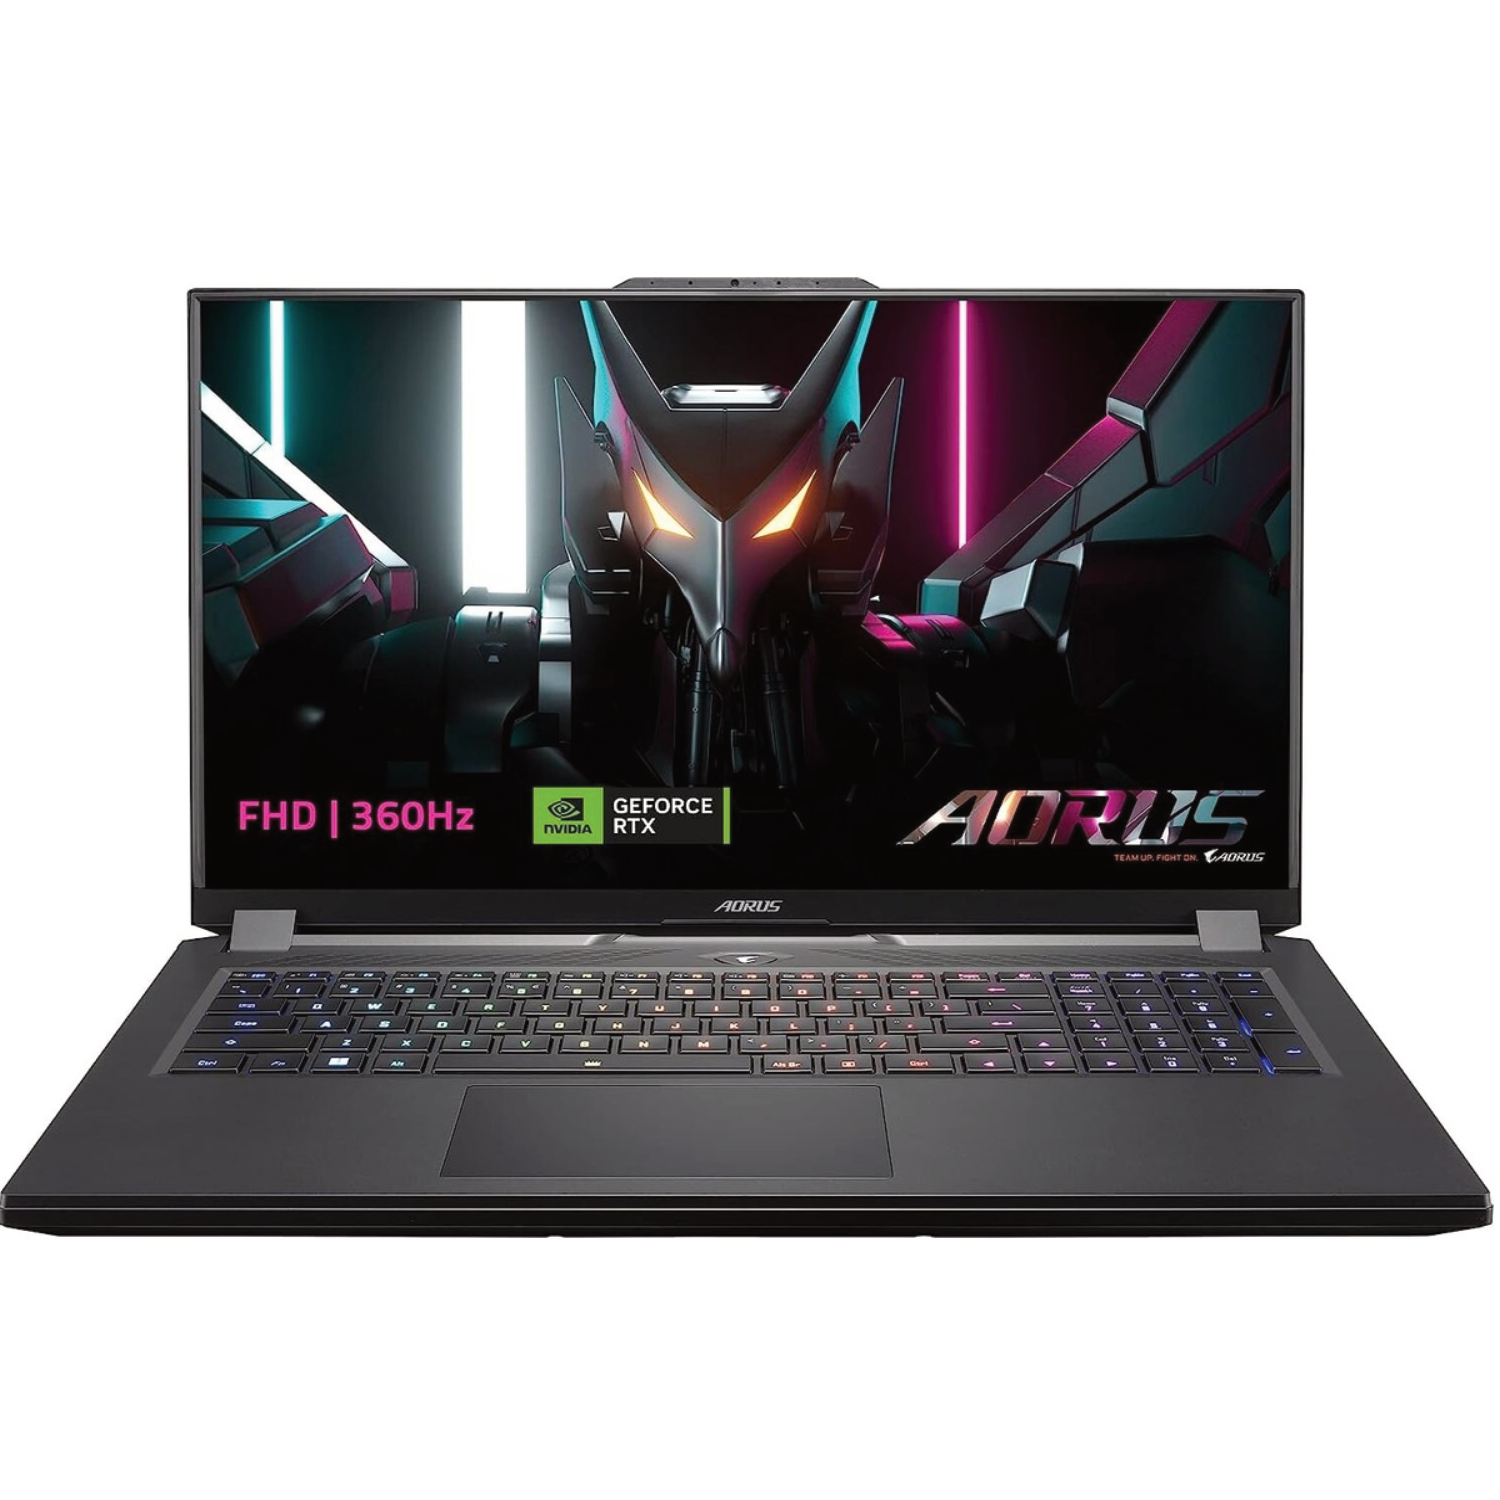
\includegraphics[height=2.5cm,keepaspectratio]{figures/Gigabyte_Aorus.png}\vspace{\fill} &
Gigabyte Aorus 7 9KF &
Processor : 12th Gen Intel(R) Core(TM) i5-12500H (2.50 GHz)

Ram : 16,0 GB

Système d'exploitation : Windows 11 Pro

Carte graphique : NVIDIA GeForce RTX 4060 Laptop GPU (8 GB) \\ \hline

\vspace{\fill}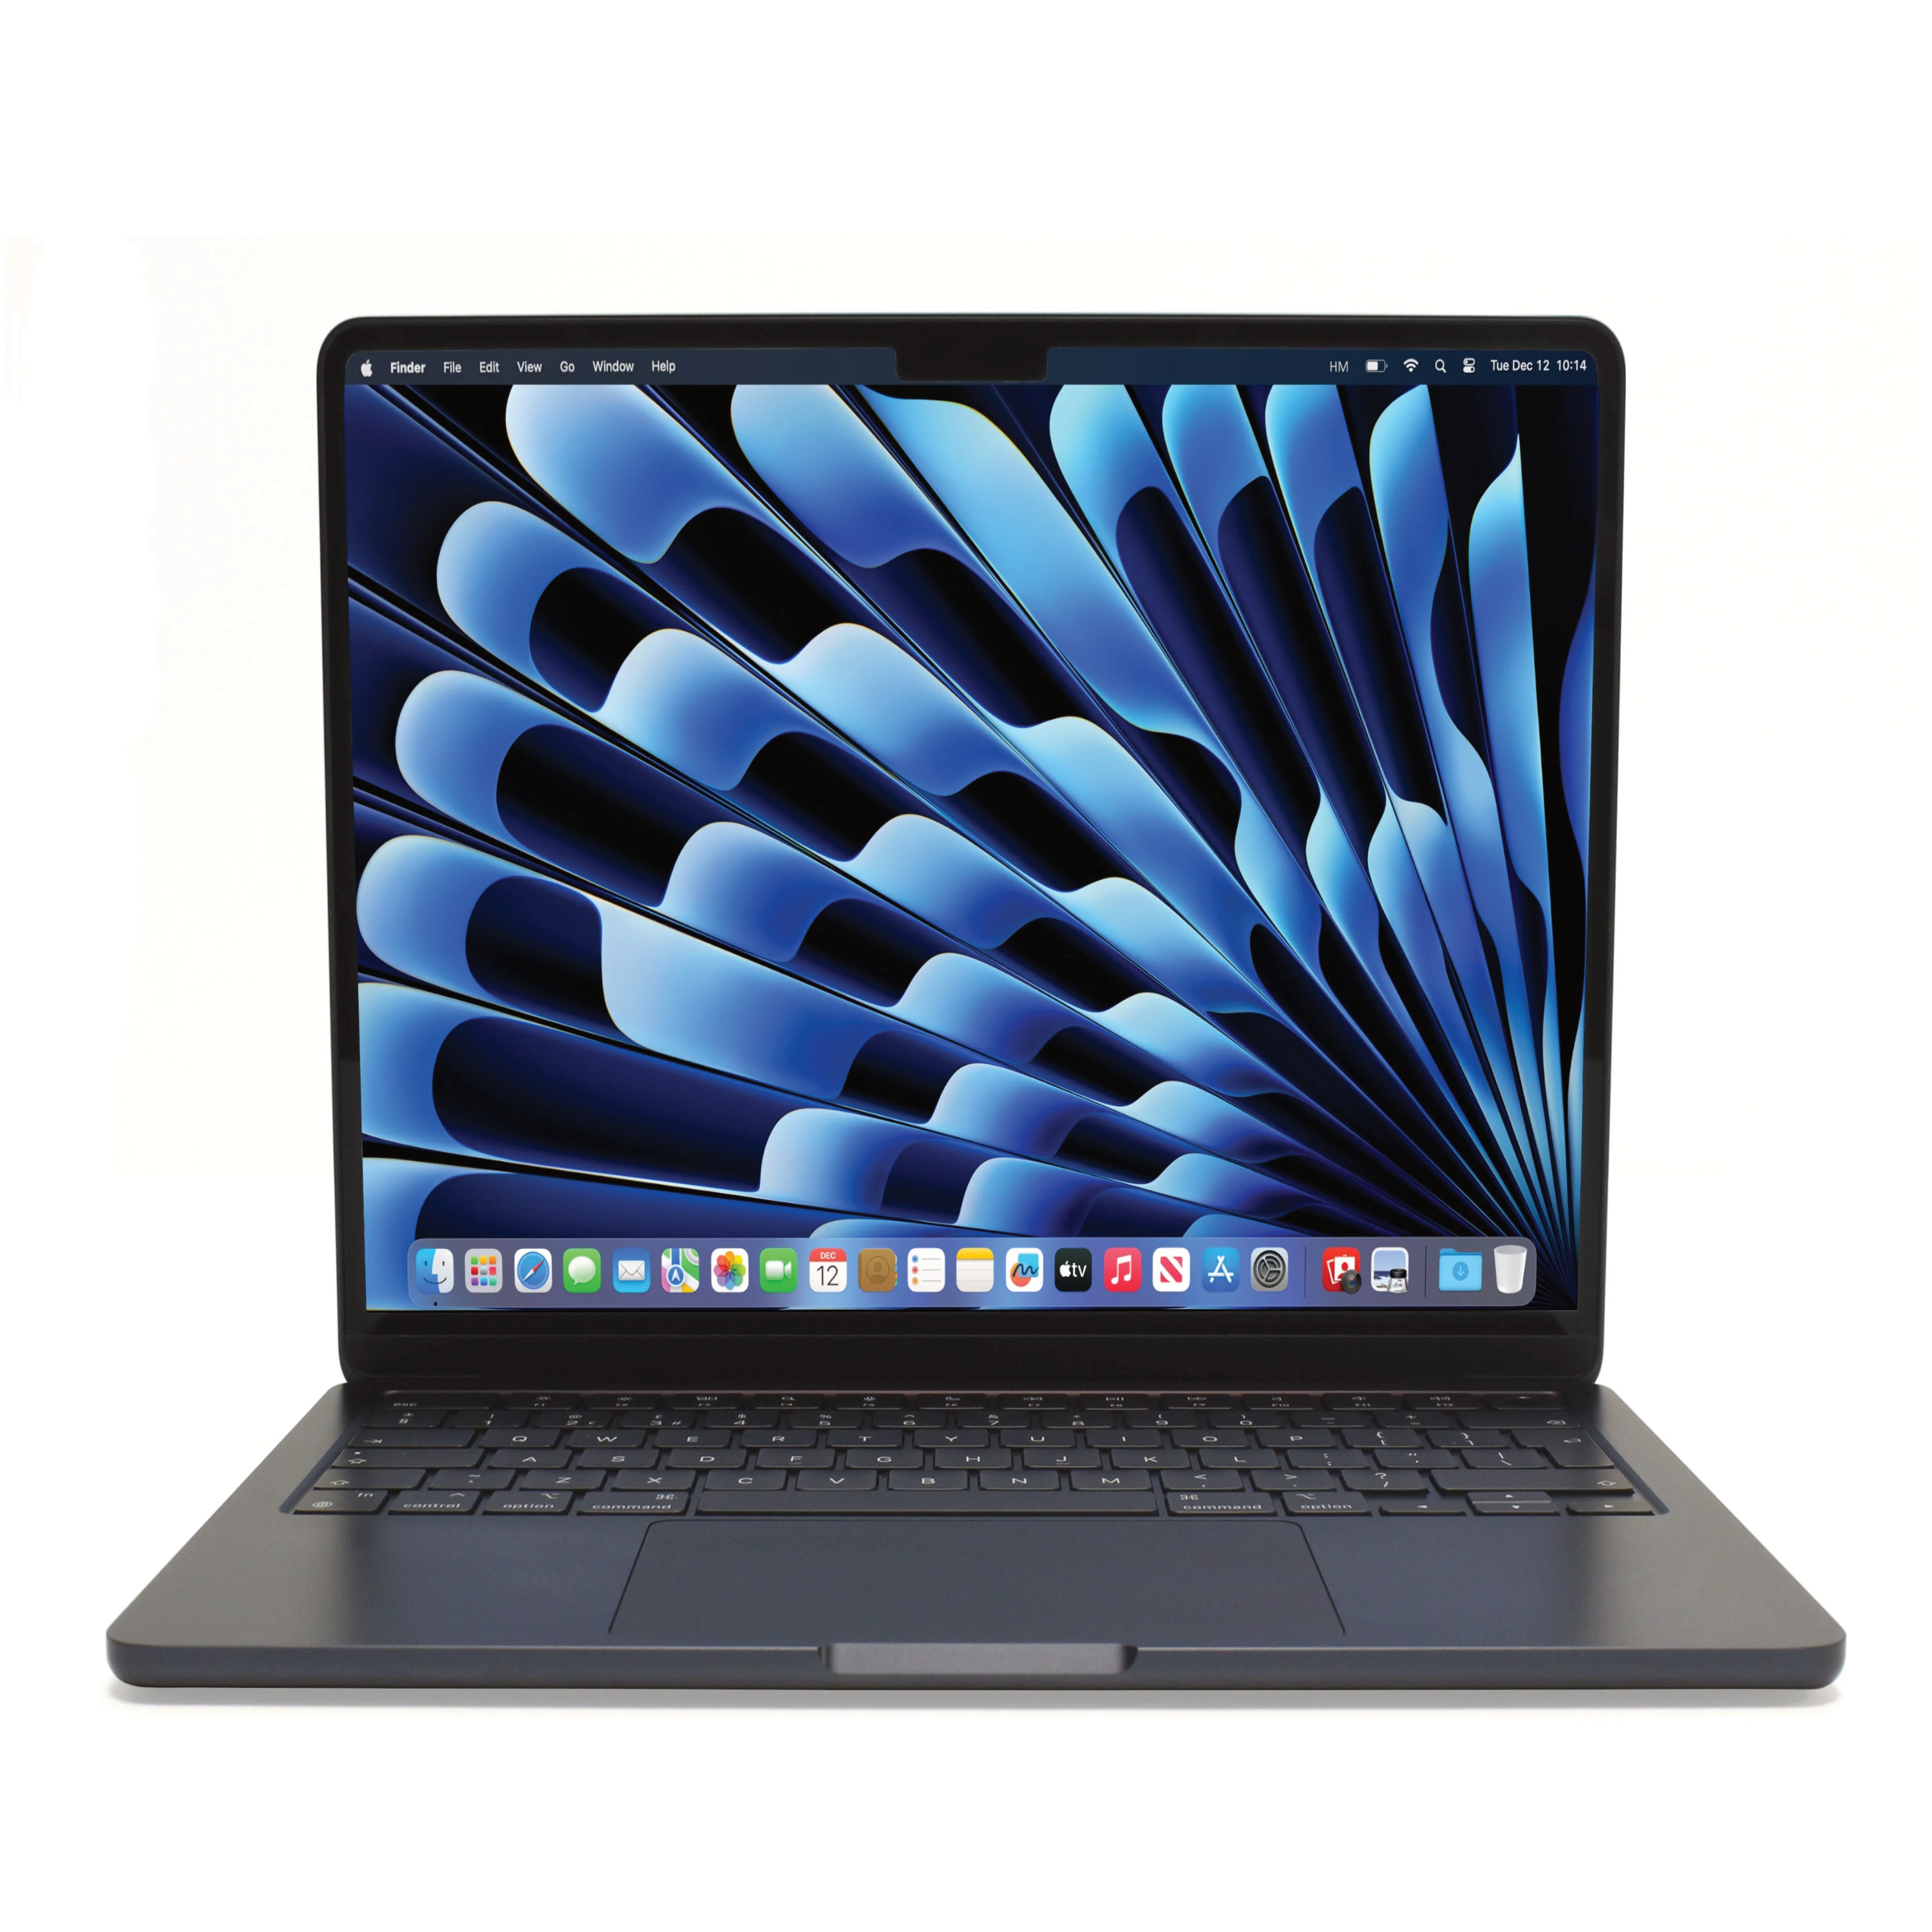
\includegraphics[height=2.5cm,keepaspectratio]{figures/macbook_air.png}\vspace{\fill} &
MacBook Air M2 &
Processor : Apple M2

Ram : 8,0 GB

Système d'exploitation : macOS Sequoia

Carte graphique : GPU intégré \\ \hline

\vspace{\fill}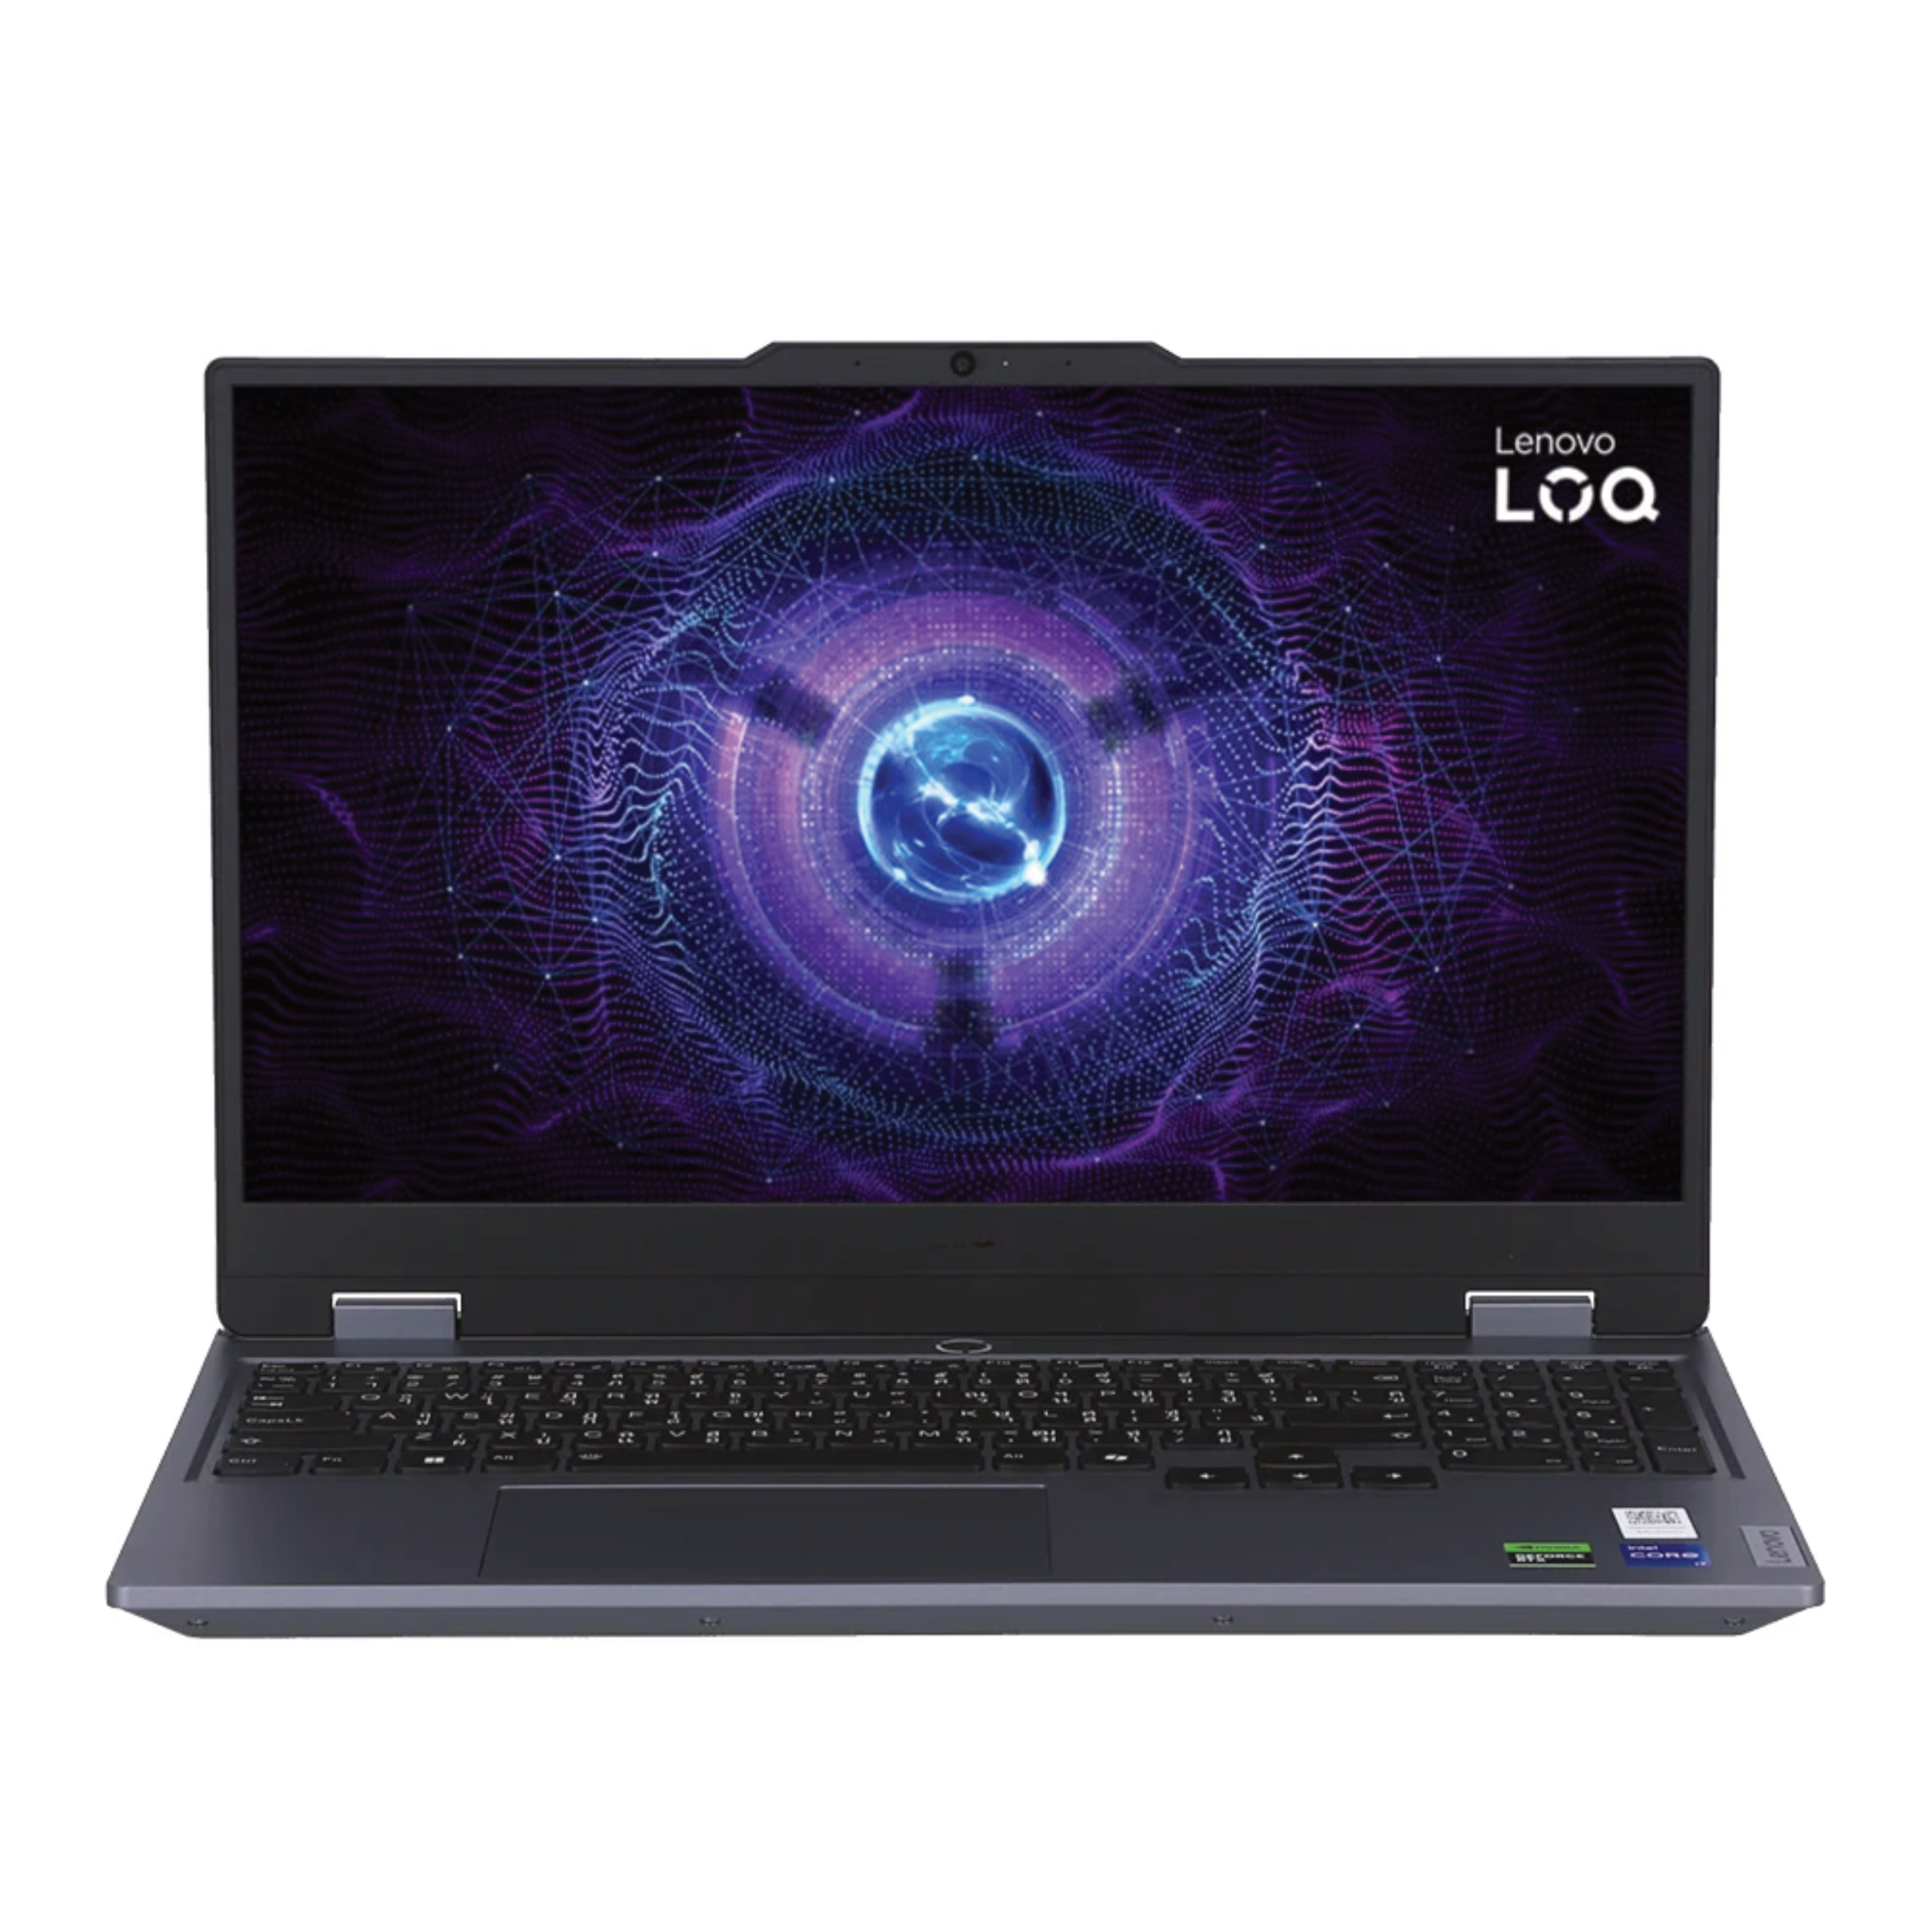
\includegraphics[height=2.5cm,keepaspectratio]{figures/Lenovo _Loq .png}\vspace{\fill} &
Lenovo Loq 15irx9 &
Processor : 13th Gen Intel(R) Core(TM) i7-13650HX (2.60 GHz)

Ram : 16,0 GB

Système d'exploitation : Windows 11 Pro

Carte graphique : NVIDIA GeForce RTX 3050 6GB Laptop GPU (6 Go) \\ \hline

\end{tabularx}
\end{table}

\subsection{Environnement logiciel}

Afin d'assurer le développement et le test efficaces de notre solution, nous avons utilisé un ensemble d'outils, de technologies et d'environnements adaptés aux besoins du projet. Cette section présente les principaux logiciels, bibliothèques et environnements de développement mobilisés tout au long de la réalisation du projet.

\subsubsection{Environnement de développement intégré:}

\subsubsection*{Visual Studio Code}

Visual Studio Code est un éditeur de code open source, gratuit et multiplateforme développé par Microsoft pour Windows, macOS et Linux. Il prend en charge plusieurs langages et technologies de développement, notamment JavaScript, TypeScript, Python, Java, C++, HTML et CSS, grâce à un vaste écosystème d'extensions. Il offre également des fonctionnalités avancées, telles que le débogage, l'intégration avec Git et diverses options de personnalisation, à travers une interface intuitive et ergonomique.

\begin{figure}[H]
	\centering
	
\includegraphics[width=0.25\textwidth]{figures/VSC.png}
	\caption{Logo de Visual Studio Code}
\end{figure}

\subsubsection*{GitHub}

GitHub est une plateforme de développement collaborative basée sur Git, permettant l'hébergement, la gestion et le partage de code source. Elle facilite le travail en équipe grâce au contrôle de version, à la gestion des branches et aux outils de collaboration tels que les pull-requests et le suivi des issues.

\begin{figure}[H]
	\centering
	
\includegraphics[width=0.25\textwidth]{figures/github.png}
	\caption{Logo de GitHub}
\end{figure}

\section{Technologies et langages de programmation utilisés}

Ce volet présente les principales technologies et langages de programmation utilisés dans le développement de la plateforme.
\subsection{Technologies de développement côté client}

Cette section présente les principales technologies utilisées pour le développement de la partie cliente de la plateforme.
\subsubsection{Angular}

Angular est un framework open source développé par Google, destiné à la création d'applications web côté client. Basé sur TypeScript, il permet de développer des applications robustes, évolutives et facilement maintenables.

\begin{figure}[H]
	\centering
	
\includegraphics[width=0.35\textwidth]{figures/angulair.png}
	\caption{Logo de Angular}
\end{figure}

\subsection{Technologies de développement côté serveur}

Cette section présente les technologies utilisées pour le développement de la partie serveur de la plateforme. 

\subsubsection{Python}

Python est un langage de programmation largement utilisé dans les domaines de la science des données, de l'analyse de données et de l'intelligence artificielle. Il se distingue par sa simplicité, sa performance et la richesse de ses bibliothèques dédiées au traitement des données textuelles et numériques, même à grande échelle. Grâce à sa flexibilité et à son vaste écosystème, Python constitue une solution adaptée aux applications de traitement et d'analyse de données.

\begin{figure}[H]
	\centering
	
\includegraphics[width=0.25\textwidth]{figures/python.png}
	\caption{Logo de Python}
\end{figure}

\subsubsection{NestJS}

NestJS est un framework open source basé sur Node.js, utilisé pour le développement d'applications serveur évolutives et maintenables. Il repose sur TypeScript et adopte une architecture modulaire inspirée d'Angular, facilitant la structuration des applications backend.

\begin{figure}[H]
	\centering
	
\includegraphics[width=0.35\textwidth]{figures/nest.png}
	\caption{Logo de NestJS}
\end{figure}

\subsubsection{Node.js}

Node.js est une plateforme logicielle open source basée sur JavaScript, conçue pour le développement d'applications réseau évolutives et fortement concurrentes, reposant sur un modèle orienté événements. Elle permet de construire des applications performantes capables de gérer un grand nombre de connexions simultanées.

\begin{figure}[H]
	\centering
	
\includegraphics[width=0.35\textwidth]{figures/node.png}
	\caption{Logo de Node.js}
\end{figure}

\subsection{Technologies de gestion des données}
Cette partie présente les technologies utilisées pour la gestion, le stockage et la manipulation des données au sein de la plateforme.
\subsubsection{MongoDB}

MongoDB est une base de données NoSQL orientée documents, conçue pour stocker et gérer des données de manière flexible et scalable. Elle utilise un format similaire au JSON (BSON), ce qui facilite le stockage de données non structurées et leur exploitation dans des applications modernes.

\begin{figure}[H]
	\centering
	
\includegraphics[width=0.35\textwidth]{figures/mongo.png}
	\caption{Logo de MongoDB}
\end{figure}

\subsubsection{PostgreSQL}

PostgreSQL est un système de gestion de bases de données relationnelles objet open source, reconnu pour sa fiabilité, son intégrité des données, ses fonctionnalités avancées et sa conformité aux standards SQL.

\begin{figure}[H]
	\centering
	
\includegraphics[width=0.25\textwidth]{figures/PostgreSQL .png}
	\caption{Logo de PostgreSQL}
\end{figure}

\subsubsection{Supabase}

Supabase est une plateforme open source de type Backend-as-a-Service (BaaS) qui fournit des services prêts à l'emploi tels qu'une base de données PostgreSQL, l'authentification, le stockage et des API automatiques pour faciliter le développement d'applications web et mobiles.

\begin{figure}[H]
	\centering
	
\includegraphics[width=0.35\textwidth]{figures/supabase.png}
	\caption{Logo de Supabase}
\end{figure}

\subsection{Outil de conception et de modélisation}
Cette partie présente l’outil utilisé pour la conception et la modélisation du système. 

\subsubsection{Draw.io}

Draw.io est un logiciel de diagramme en ligne gratuit permettant de concevoir différents types de schémas, notamment des diagrammes UML, des diagrammes de processus, des modèles entités-associations, des organigrammes et des diagrammes de réseau. Il est largement utilisé pour la modélisation et la documentation des systèmes informatiques.

\begin{figure}[H]
	\centering
	
\includegraphics[width=0.25\textwidth]{figures/digrammes.png}
	\caption{Logo de Draw.io}
\end{figure}

\subsection{Service d'intelligence artificielle}
Cette partie présente le service d’intelligence artificielle intégré à la plateforme. 

\subsubsection{Gemini API}

Gemini API est une interface de programmation proposée par Google permettant d'accéder aux modèles d'intelligence artificielle Gemini. Elle offre des fonctionnalités de génération de texte, d'analyse de contenu et de compréhension multimodale (texte, image, etc.), facilitant leur intégration dans des applications.

\begin{figure}[H]
	\centering
	
\includegraphics[width=0.35\textwidth]{figures/gemini.png}
	\caption{Logo de Gemini API}
\end{figure}

\section{Principales interfaces graphiques}

Cette section est dédiée à la présentation des interfaces graphiques développées au cours de notre projet. Ces interfaces permettent de visualiser de manière intuitive l'ensemble de nos modules fonctionnels : la génération du CV ATS, l'évaluation des scores actuels ATS et employabilité, ainsi que le score d'employabilité prévisionnel après l'obtention des certifications recommandées.

\subsection{Authentification}

La figure~\ref{fig:acces-academique-professionnel} ci-dessous illustre l'interface d'authentification de la plateforme, où l'étudiant et l'administrateur se connectent via l'accès académique, tandis que les sociétés utilisent l'accès professionnel.

\begin{figure}[H]
\centering
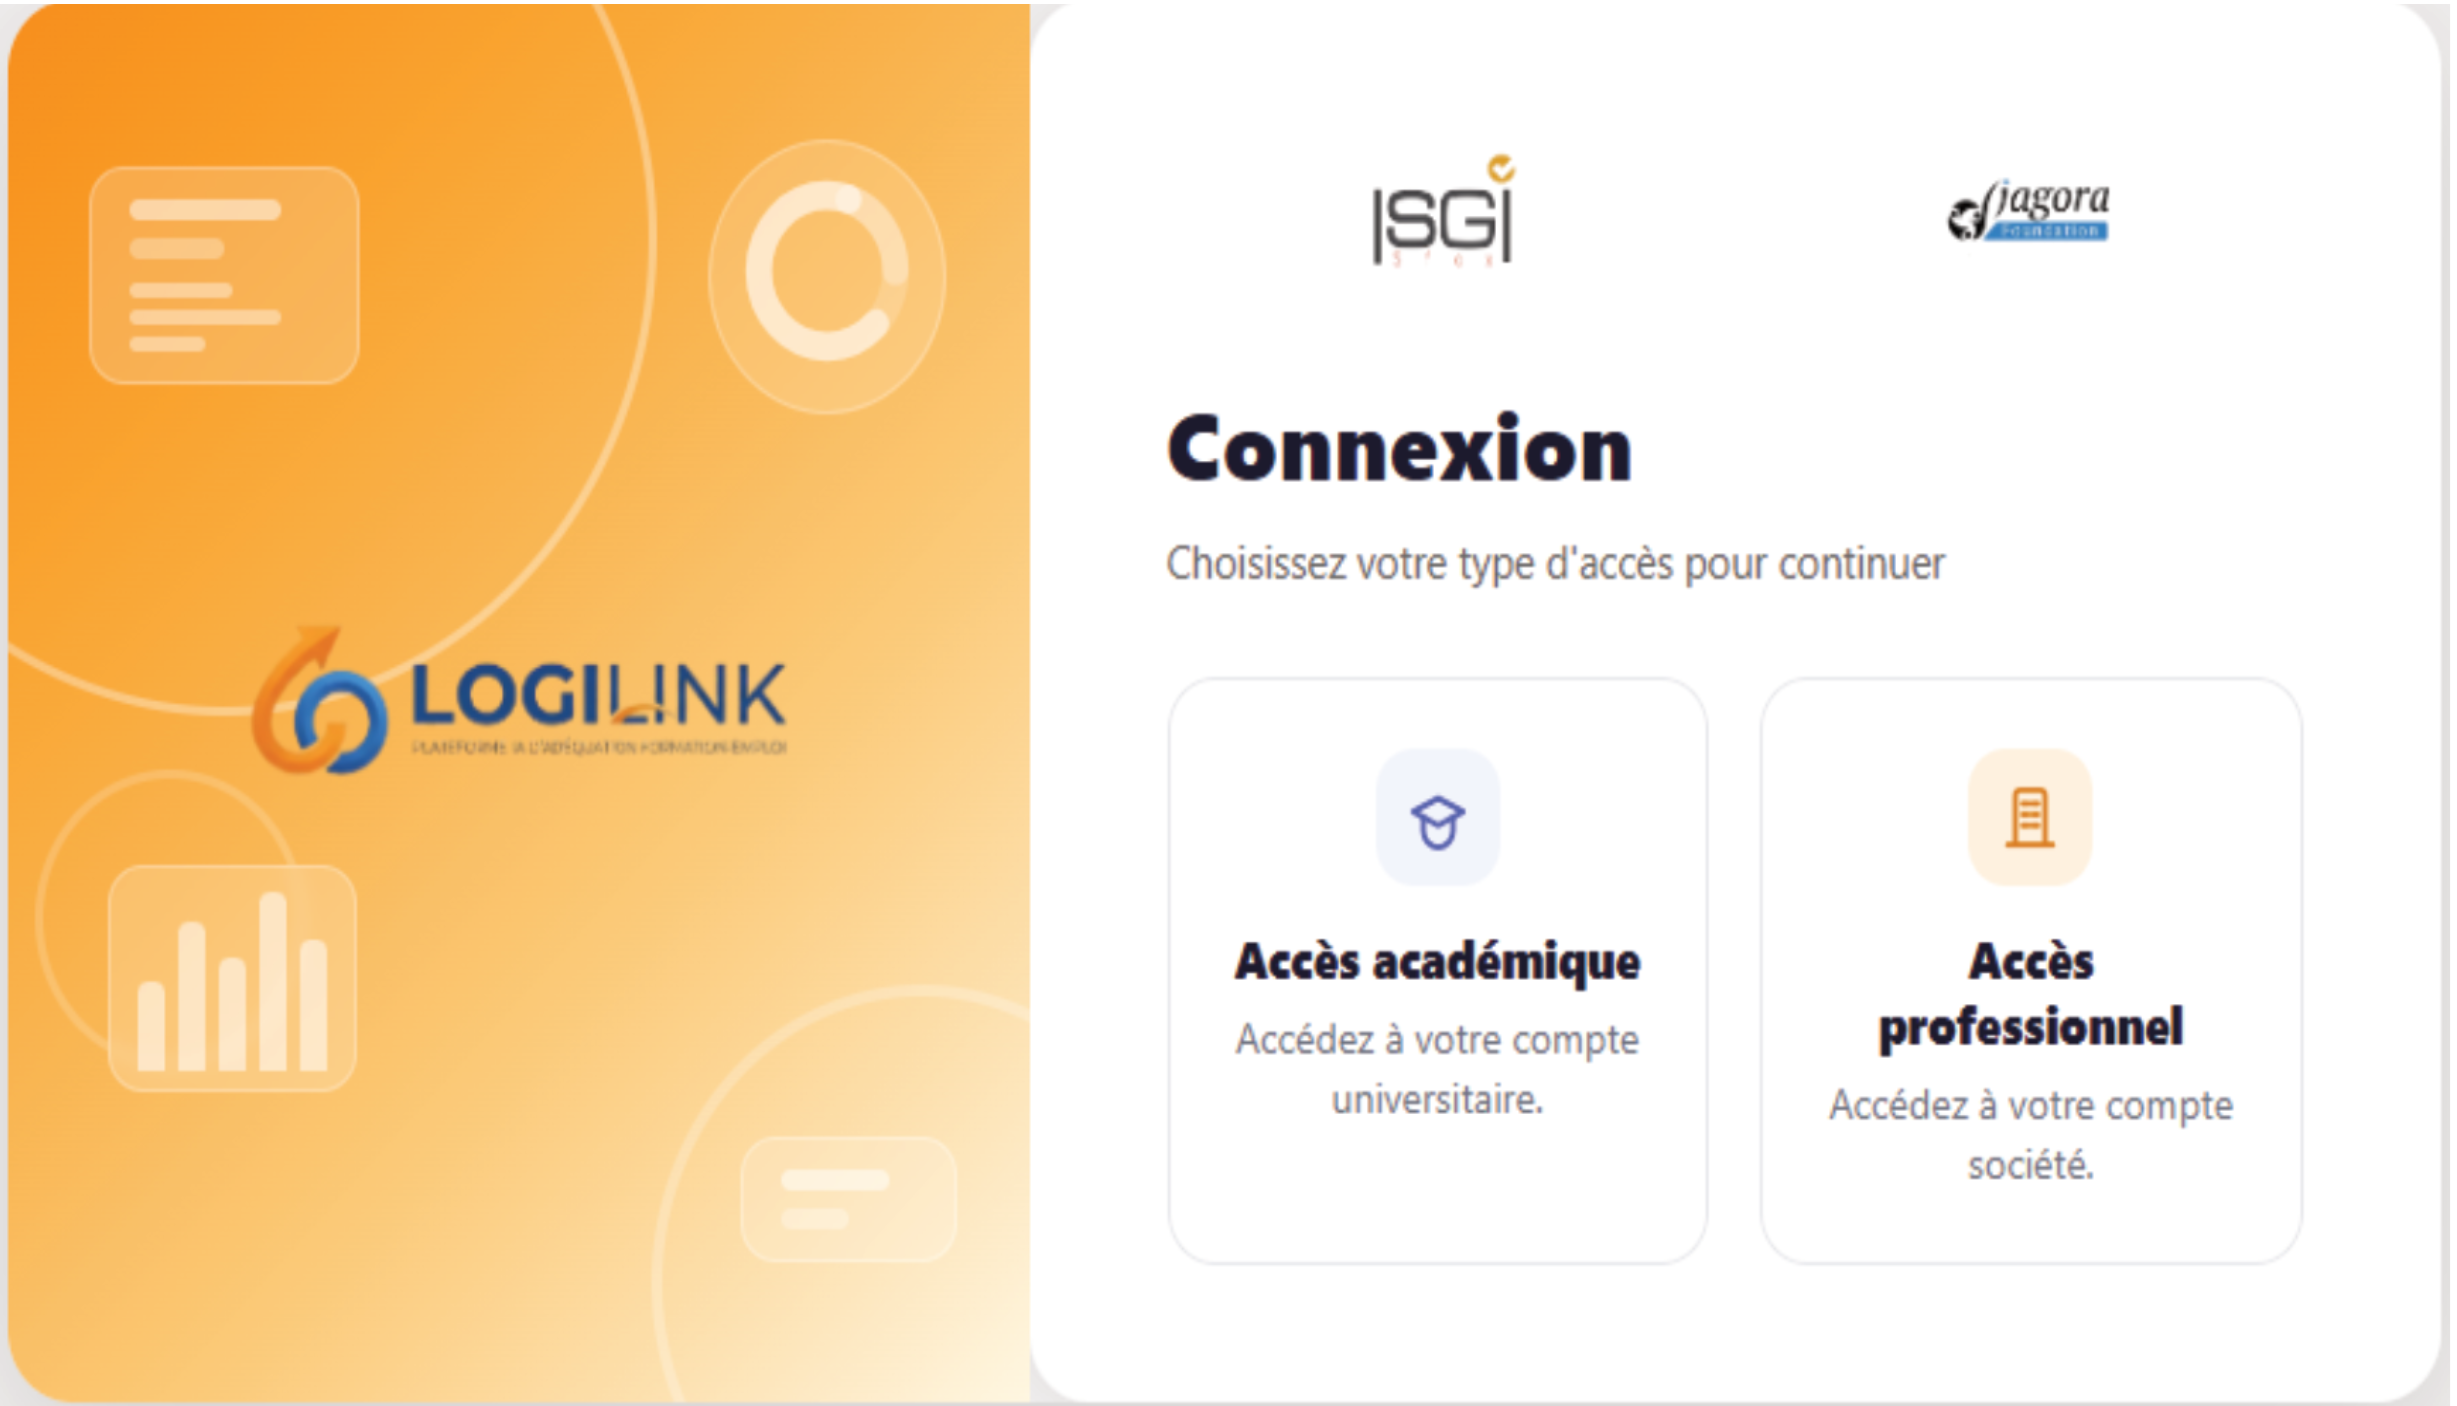
\includegraphics[width=0.85\textwidth]{figures/Interface_daacces_academique_et_professionnel.png}
\caption{Interface d'accès académique et professionnel}
\label{fig:acces-academique-professionnel}
\end{figure}

\noindent La figure~\ref{fig:authentification} indique que pour s'authentifier, l'étudiant ou l'administrateur doit simplement saisir son identifiant et son mot de passe.

\begin{figure}[H]
\centering
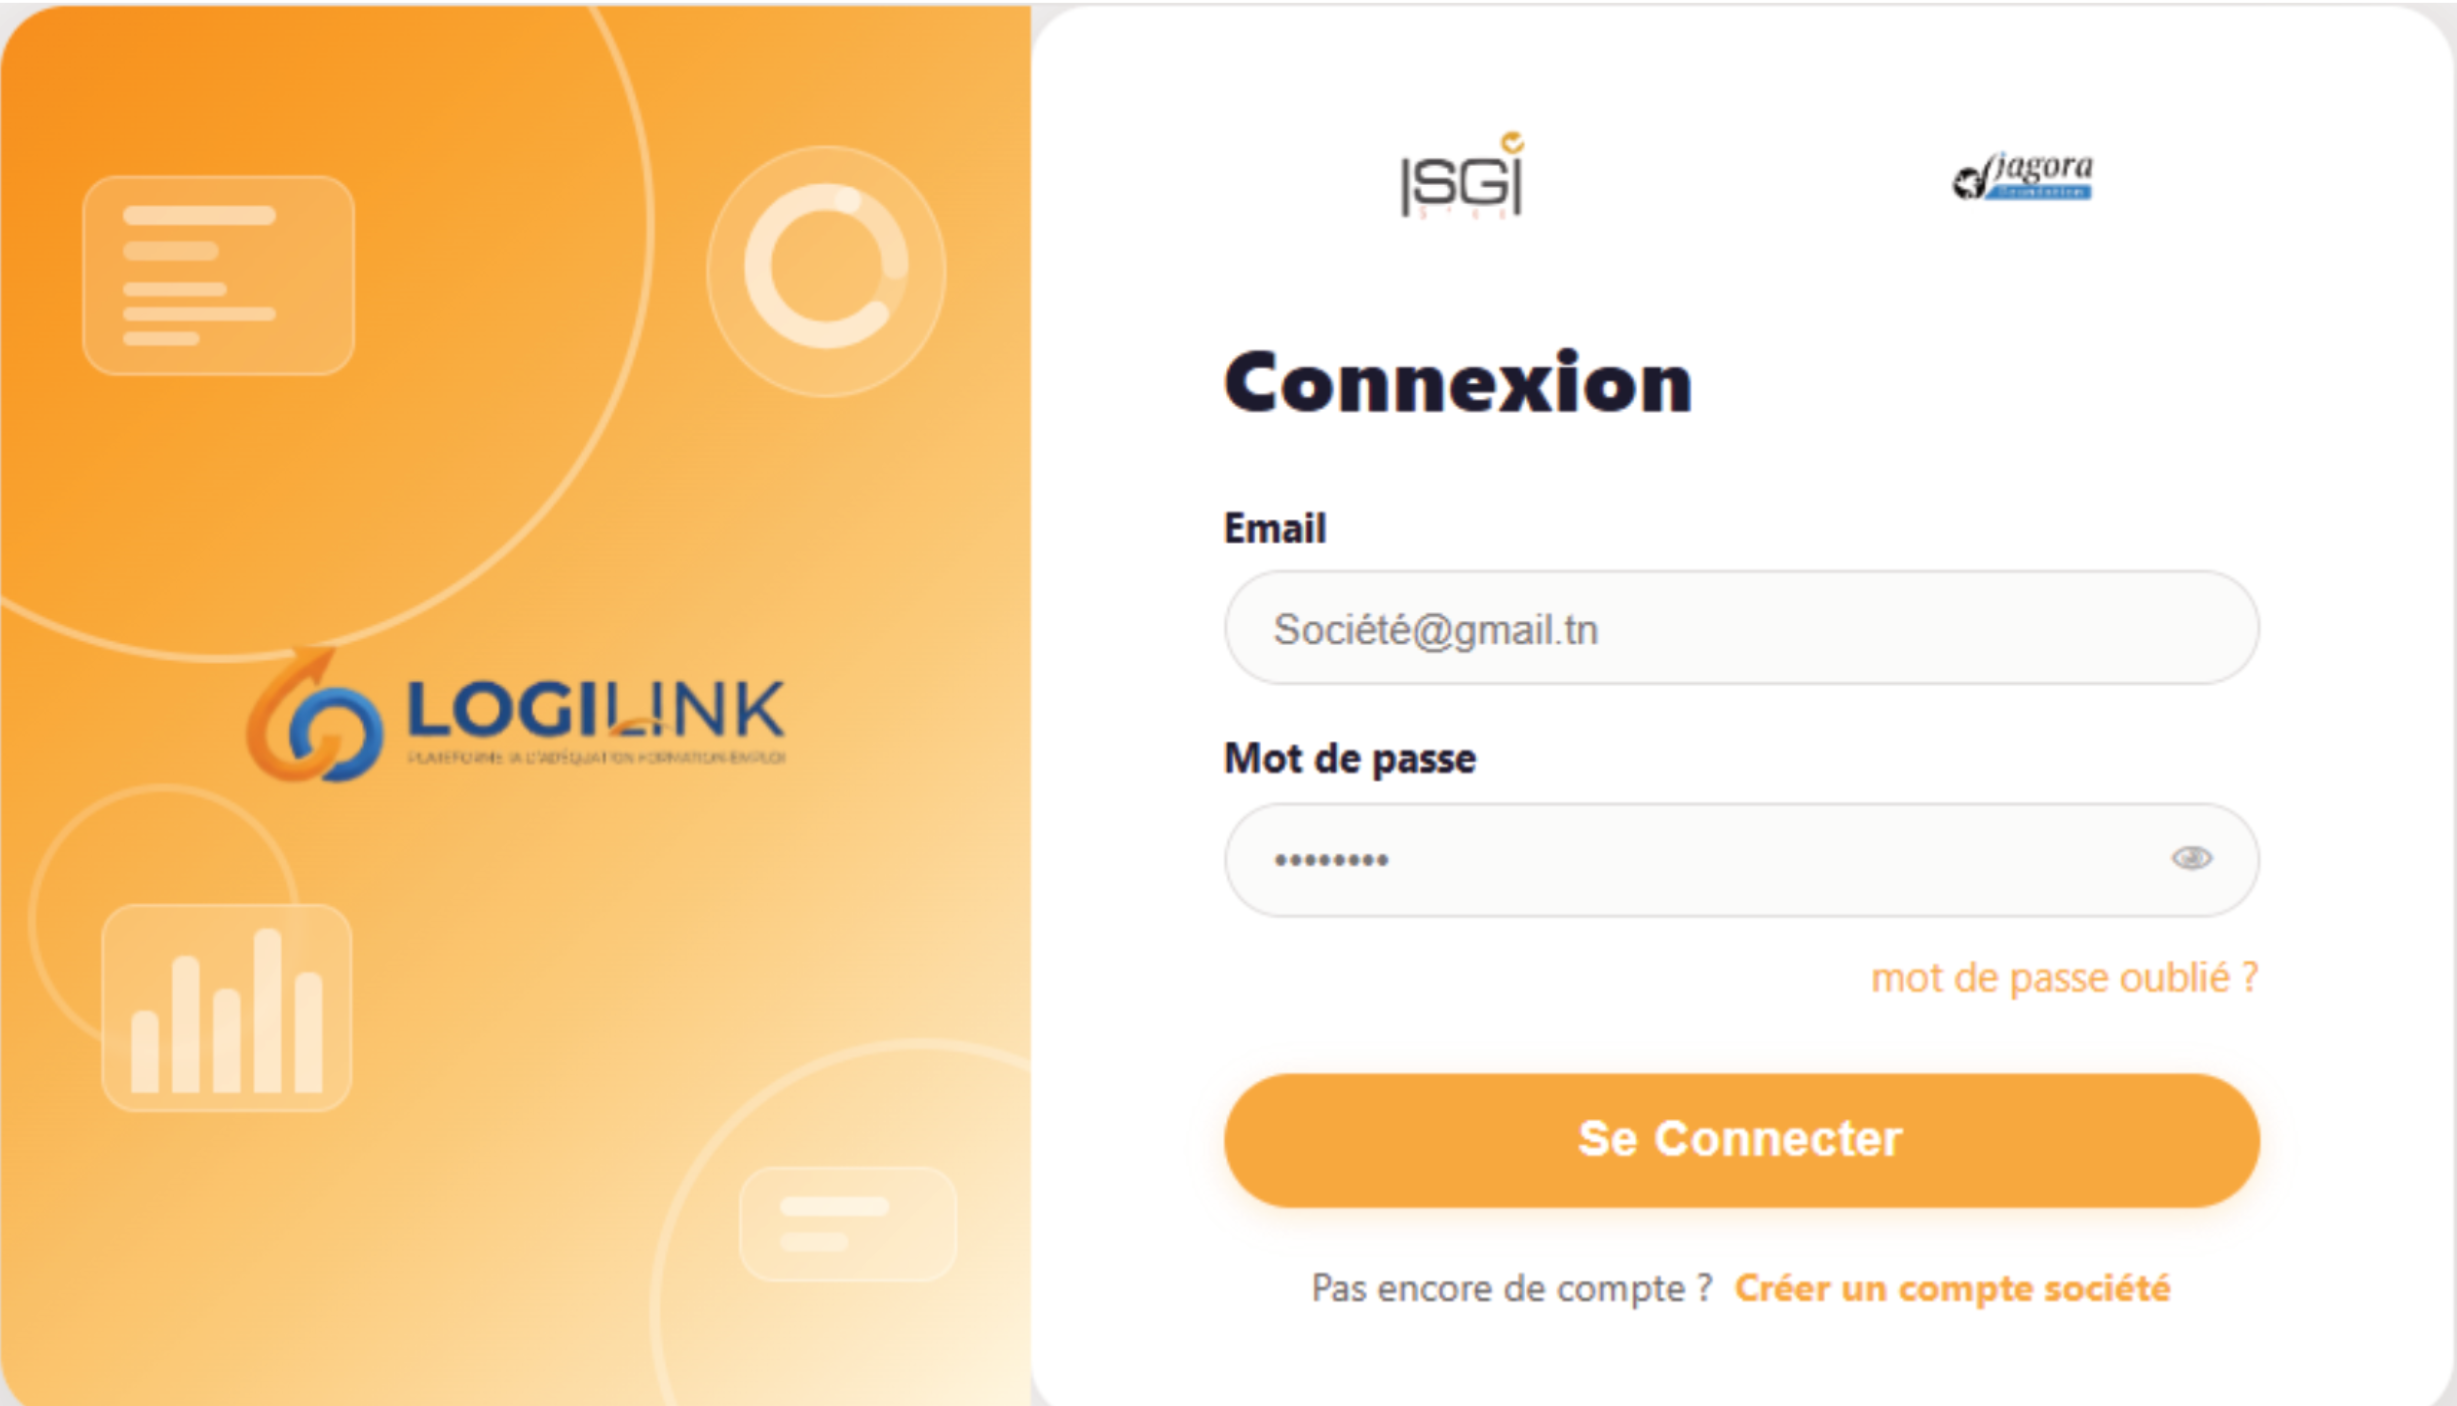
\includegraphics[width=0.85\textwidth]{figures/Interface_daauthentification.png}
\caption{Interface d'authentification}
\label{fig:authentification}
\end{figure}

\noindent La figure~\ref{fig:verification-identite} ci-dessous illustre l'étape de vérification de l'identité de l'étudiant. Après la saisie de son identifiant et de son mot de passe, un code de vérification à six chiffres est envoyé à son adresse e-mail afin de confirmer son identité.

\begin{figure}[H]
\centering
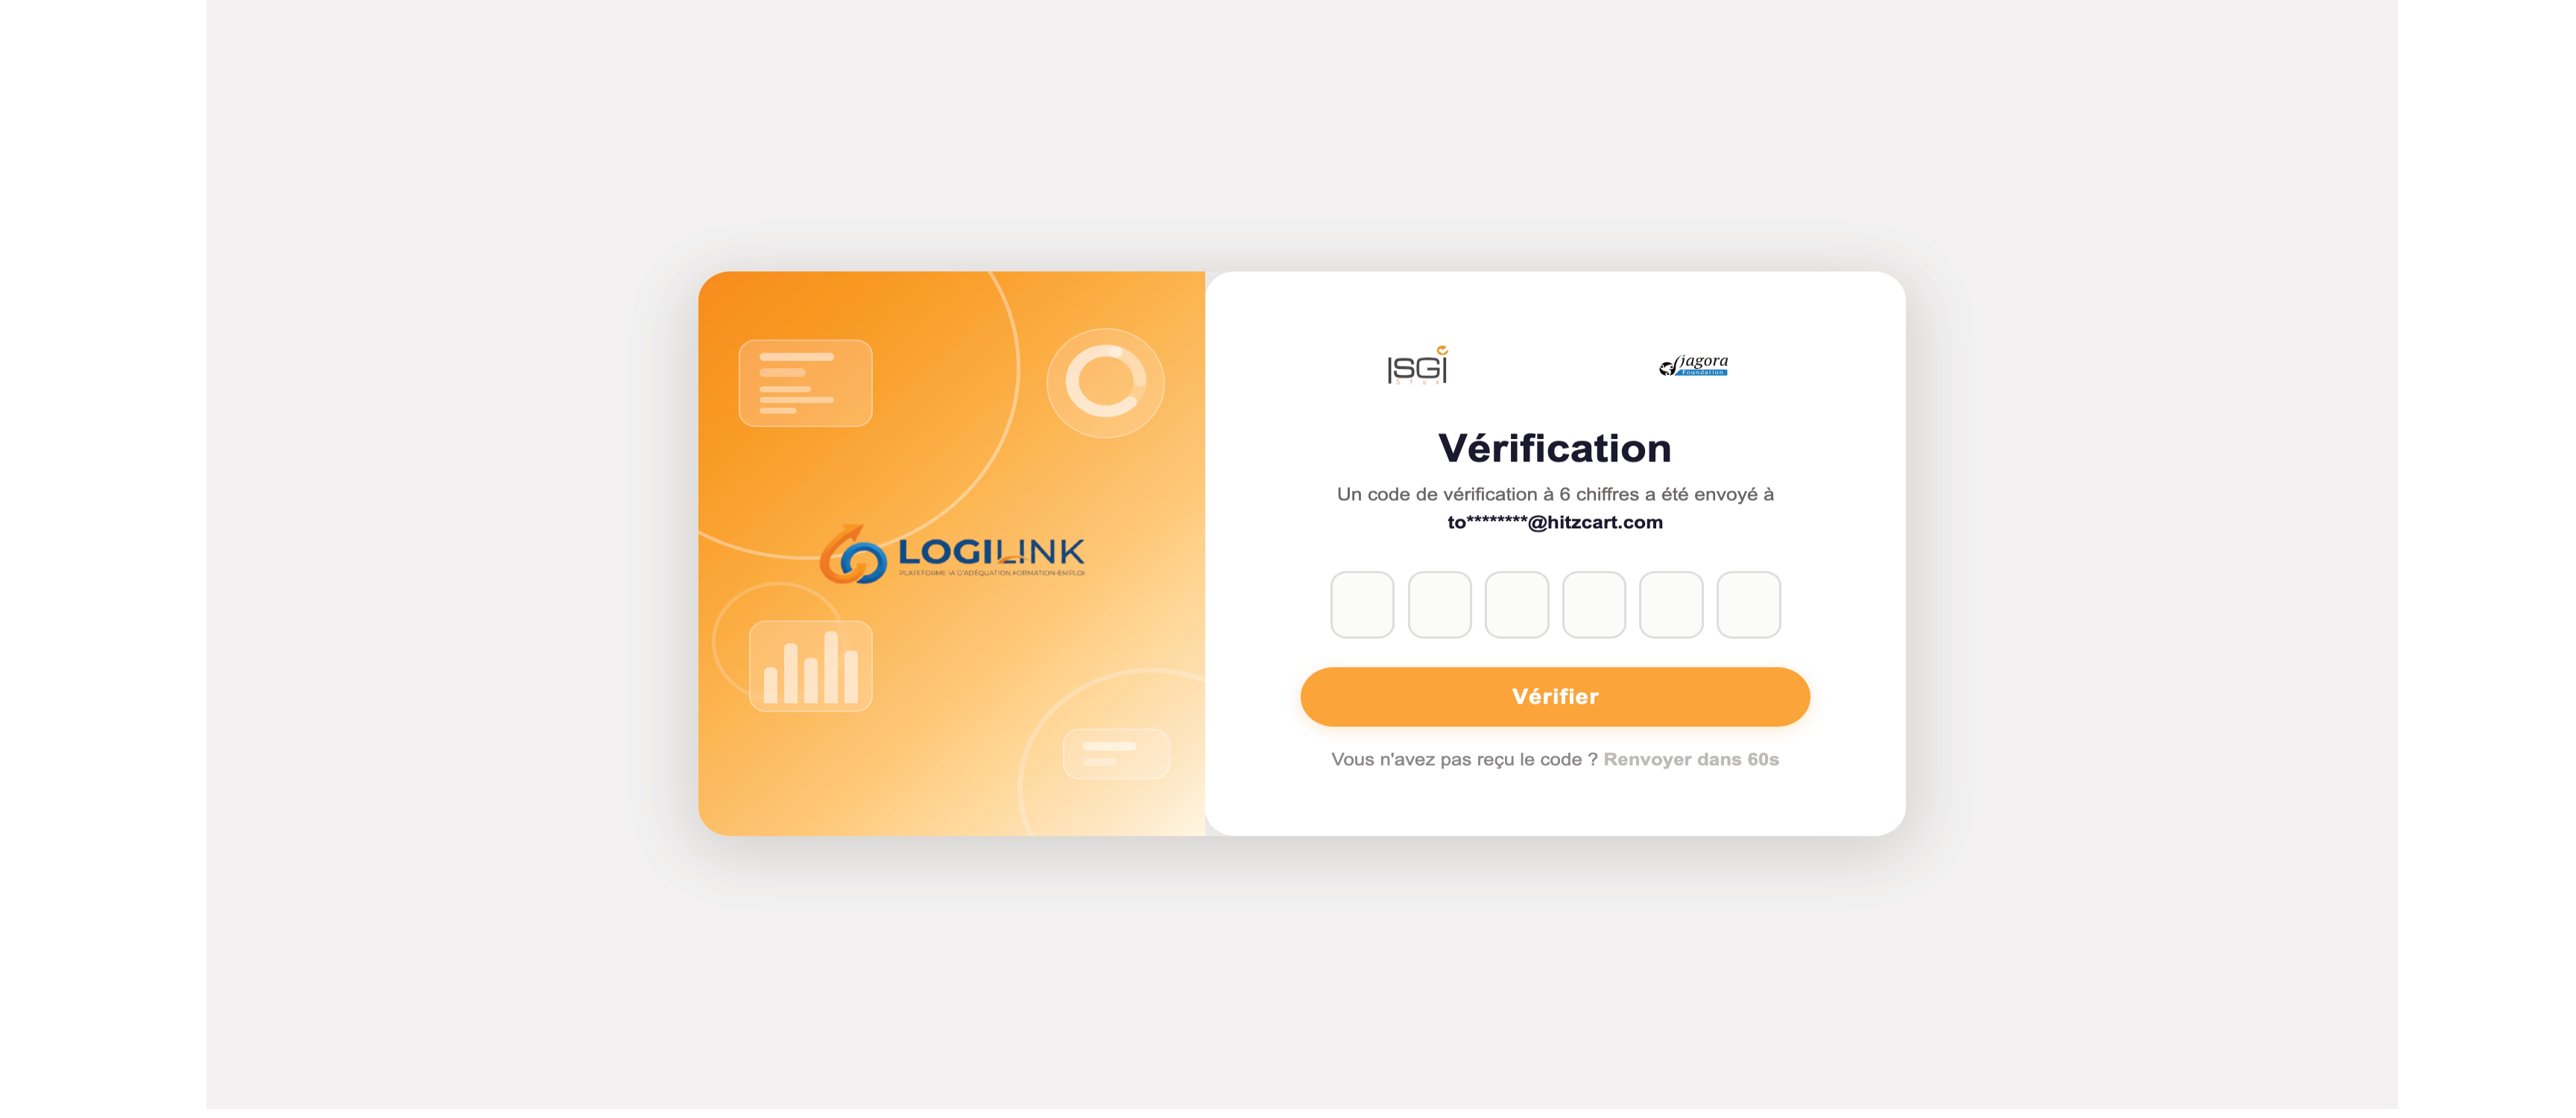
\includegraphics[width=0.85\textwidth]{figures/Interface_de_verification_daidentite.png}
\caption{Interface de vérification d'identité}
\label{fig:verification-identite}
\end{figure}

\noindent La figure~\ref{fig:creation-compte-societe} ci-dessous illustre l'interface d'inscription permettant à une société de créer un compte en renseignant ses informations professionnelles.

\begin{figure}[H]
\centering
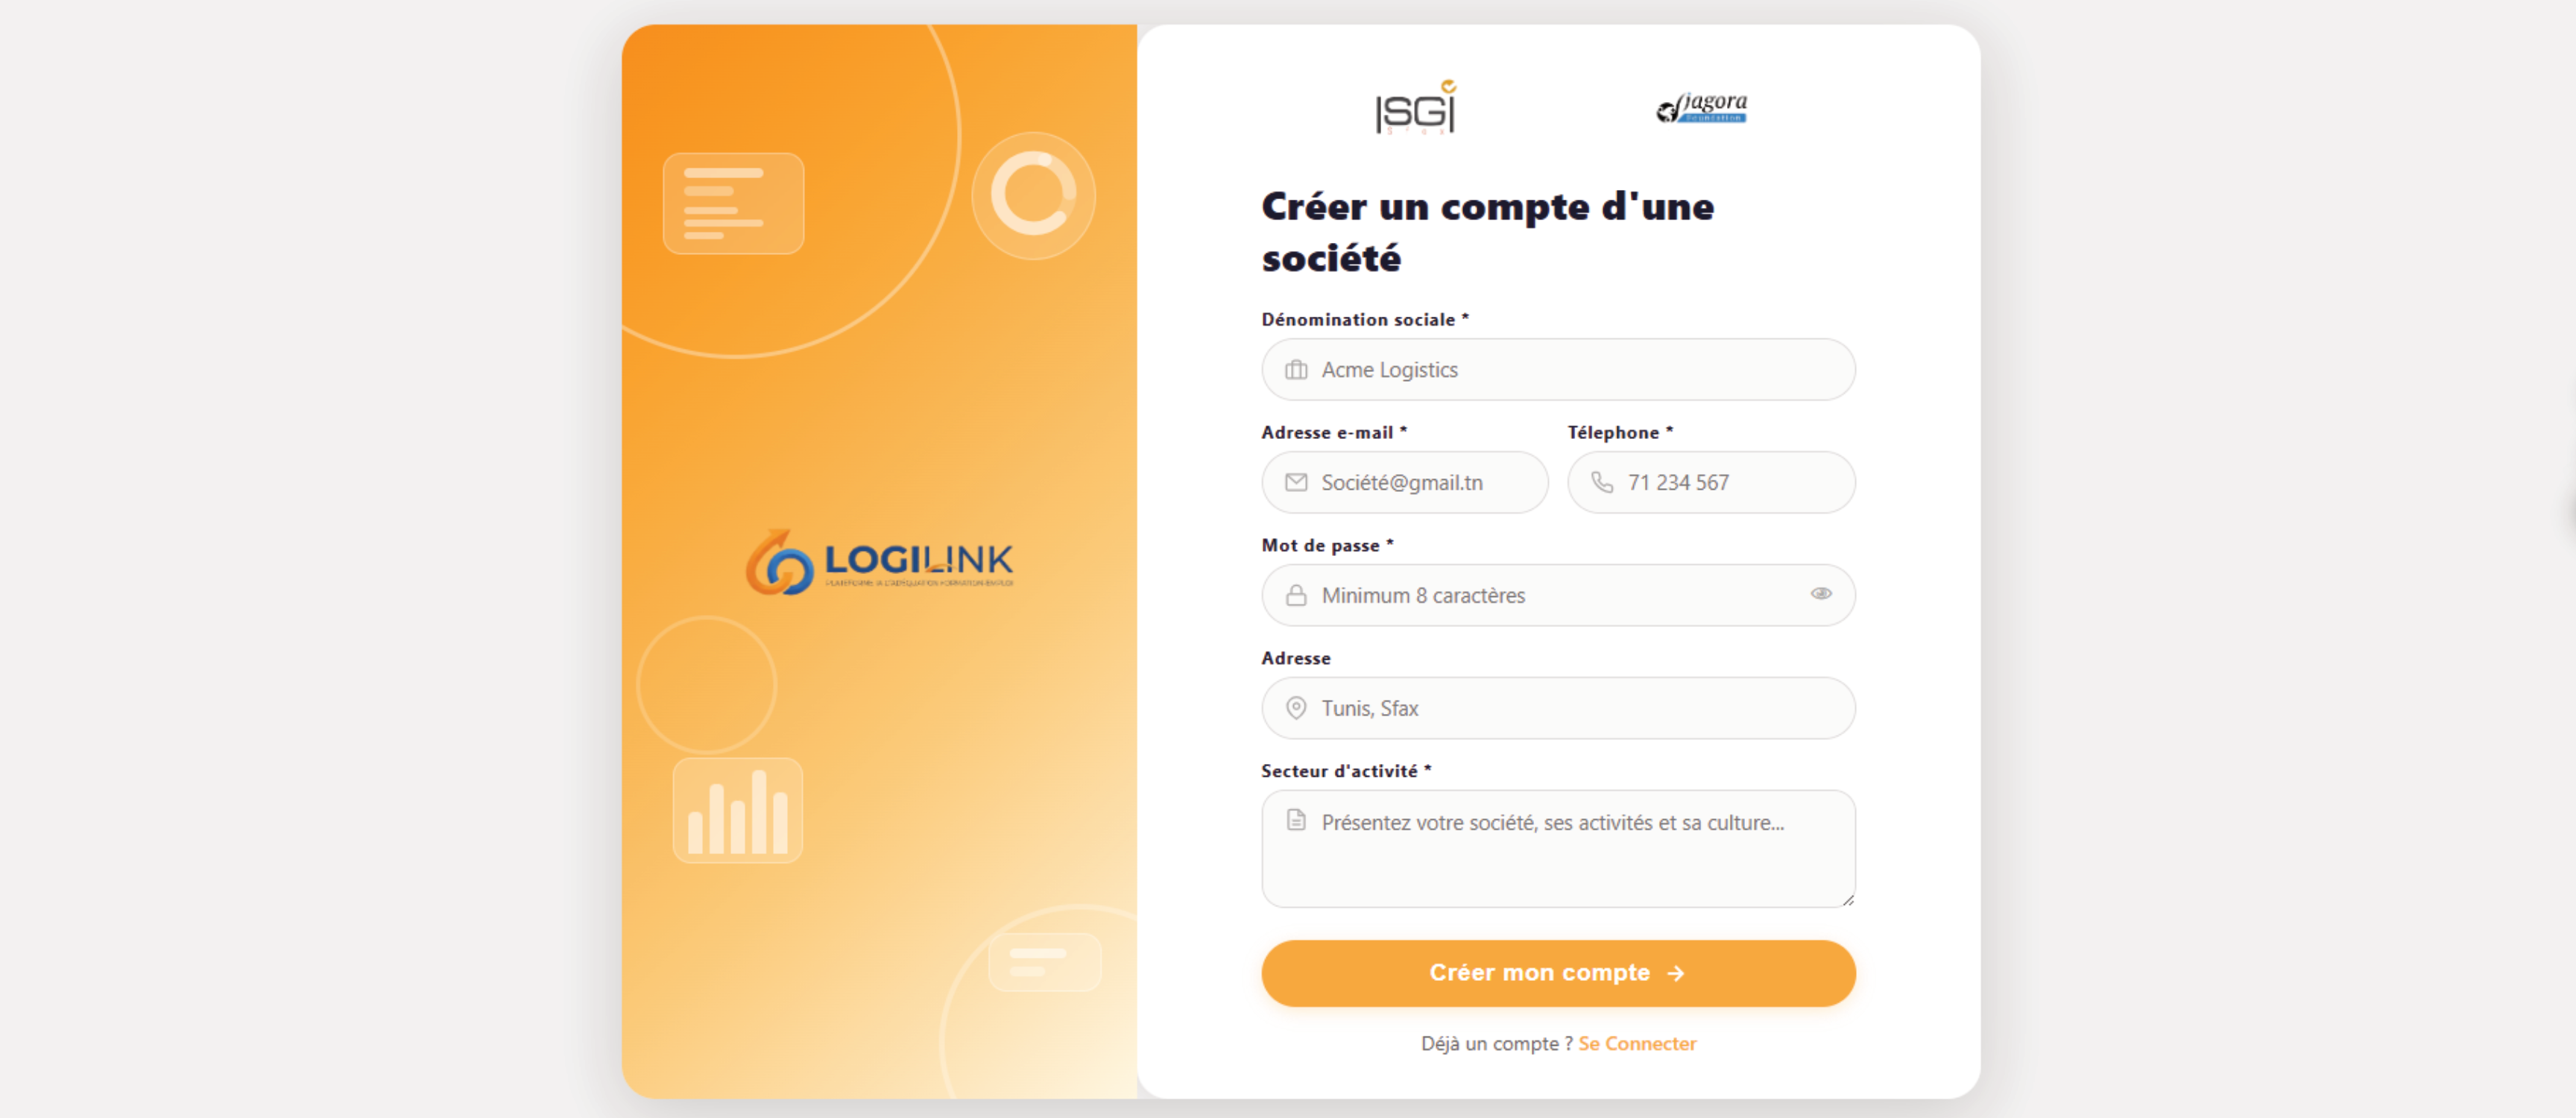
\includegraphics[width=0.85\textwidth]{figures/Interface_de_creation_de_compte_societe.png}
\caption{Interface de création de compte société}
\label{fig:creation-compte-societe}
\end{figure}

\noindent La figure~\ref{fig:authentification-societe} ci-dessous, il suffit à la société de saisir son adresse e-mail et son mot de passe pour s'authentifier.

\begin{figure}[H]
\centering
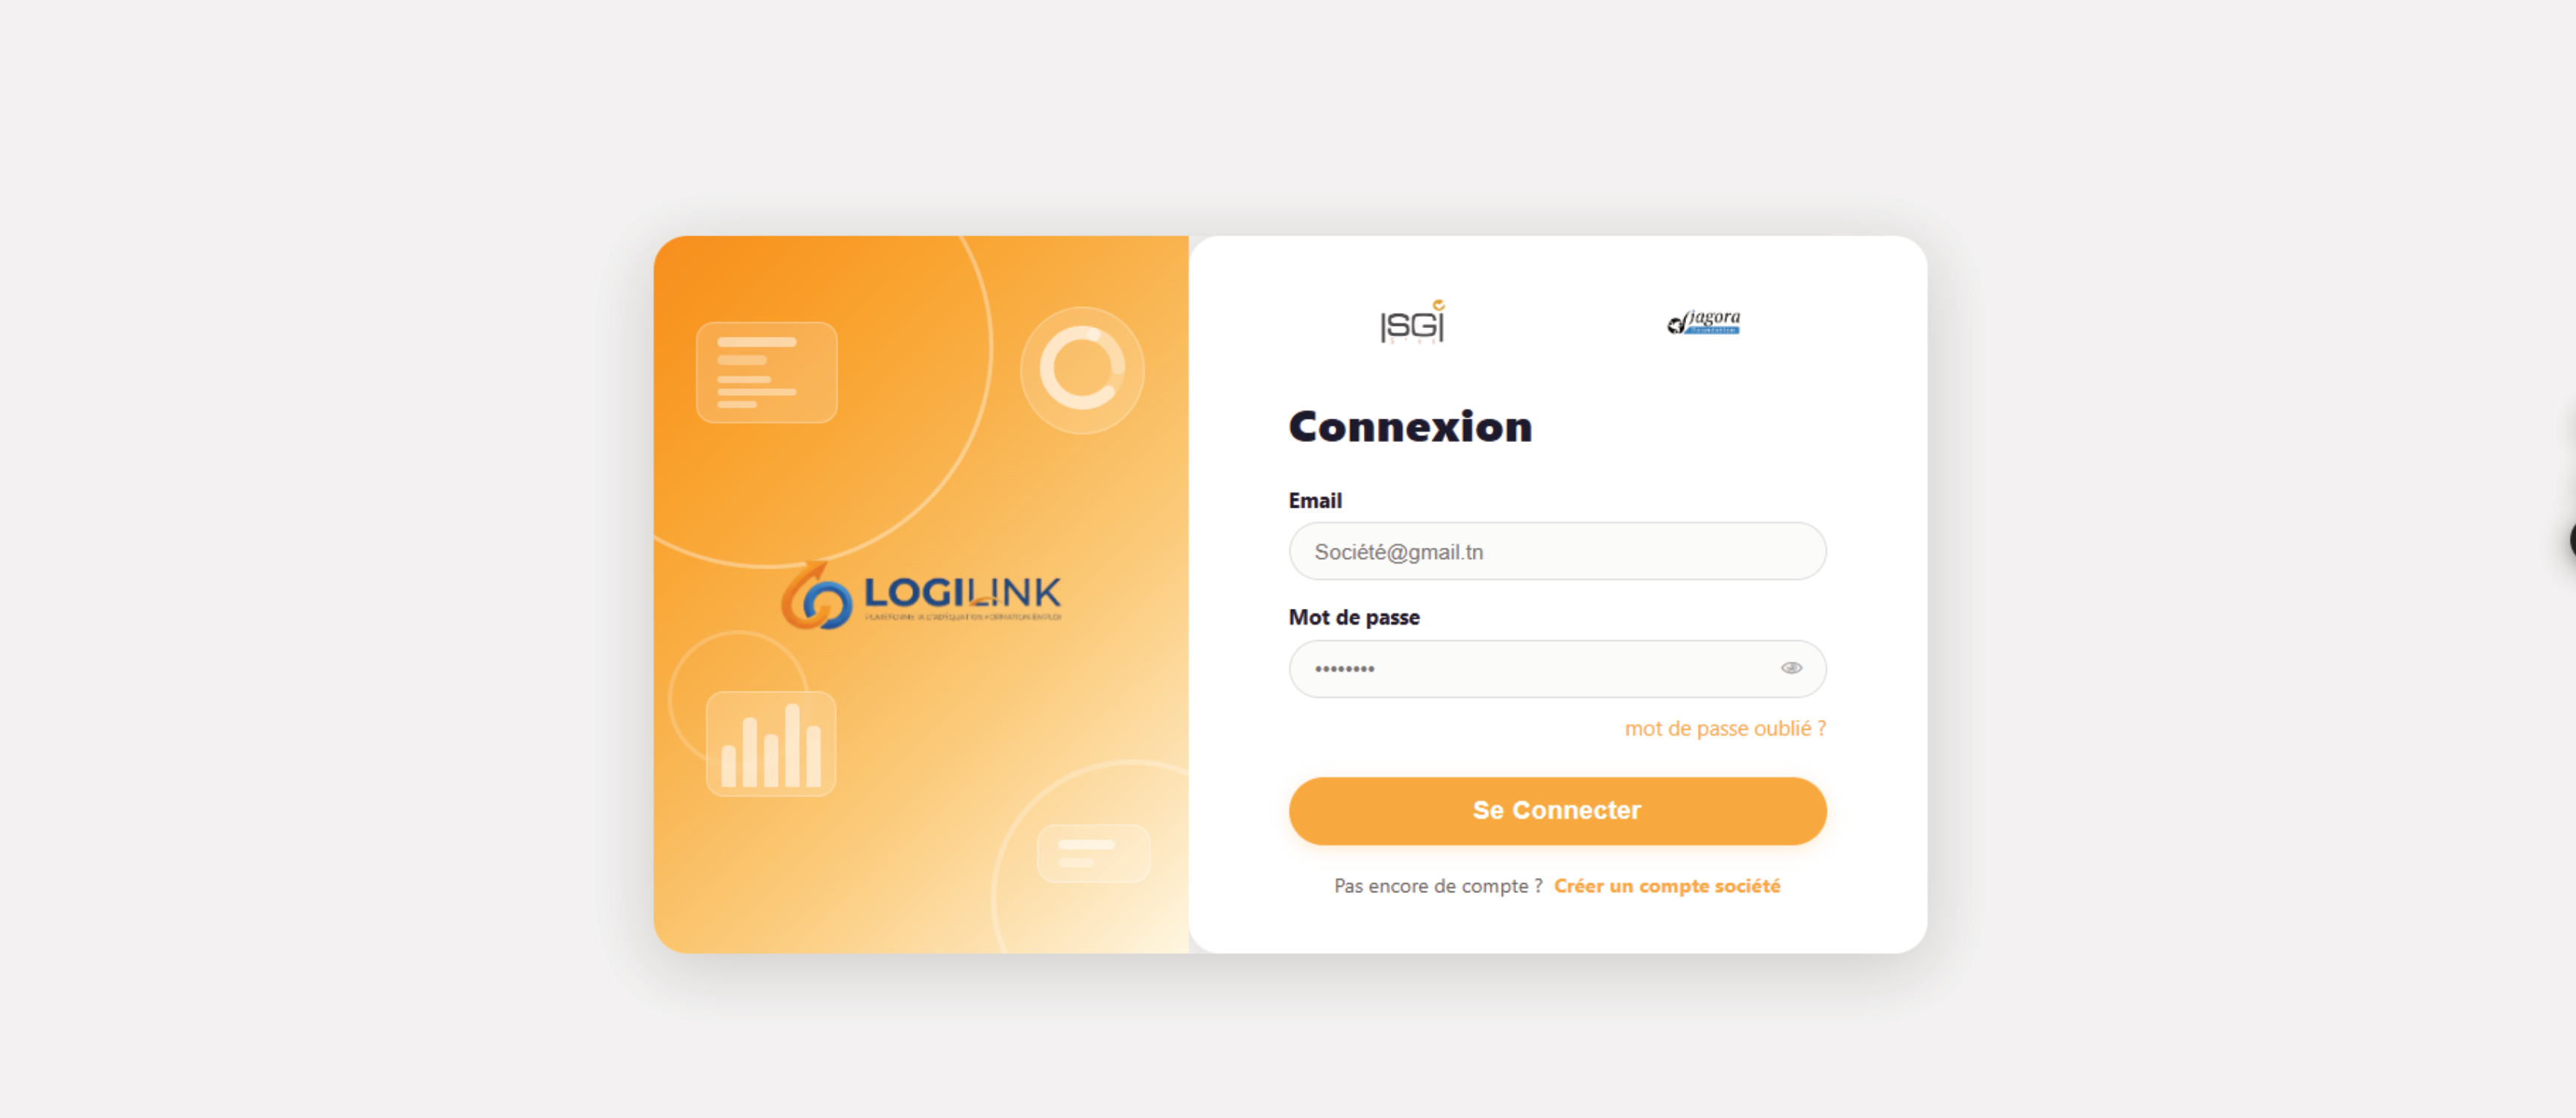
\includegraphics[width=0.85\textwidth]{figures/Interface_daauthentification_des_societes.png}
\caption{Interface d'authentification des sociétés}
\label{fig:authentification-societe}
\end{figure}

\subsection{Interfaces étudiant}

\subsubsection{Profil étudiant}

\noindent La figure~\ref{fig:profil-etudiant} ci-dessous affiche les informations personnelles de l'étudiant.

\begin{figure}[H]
\centering
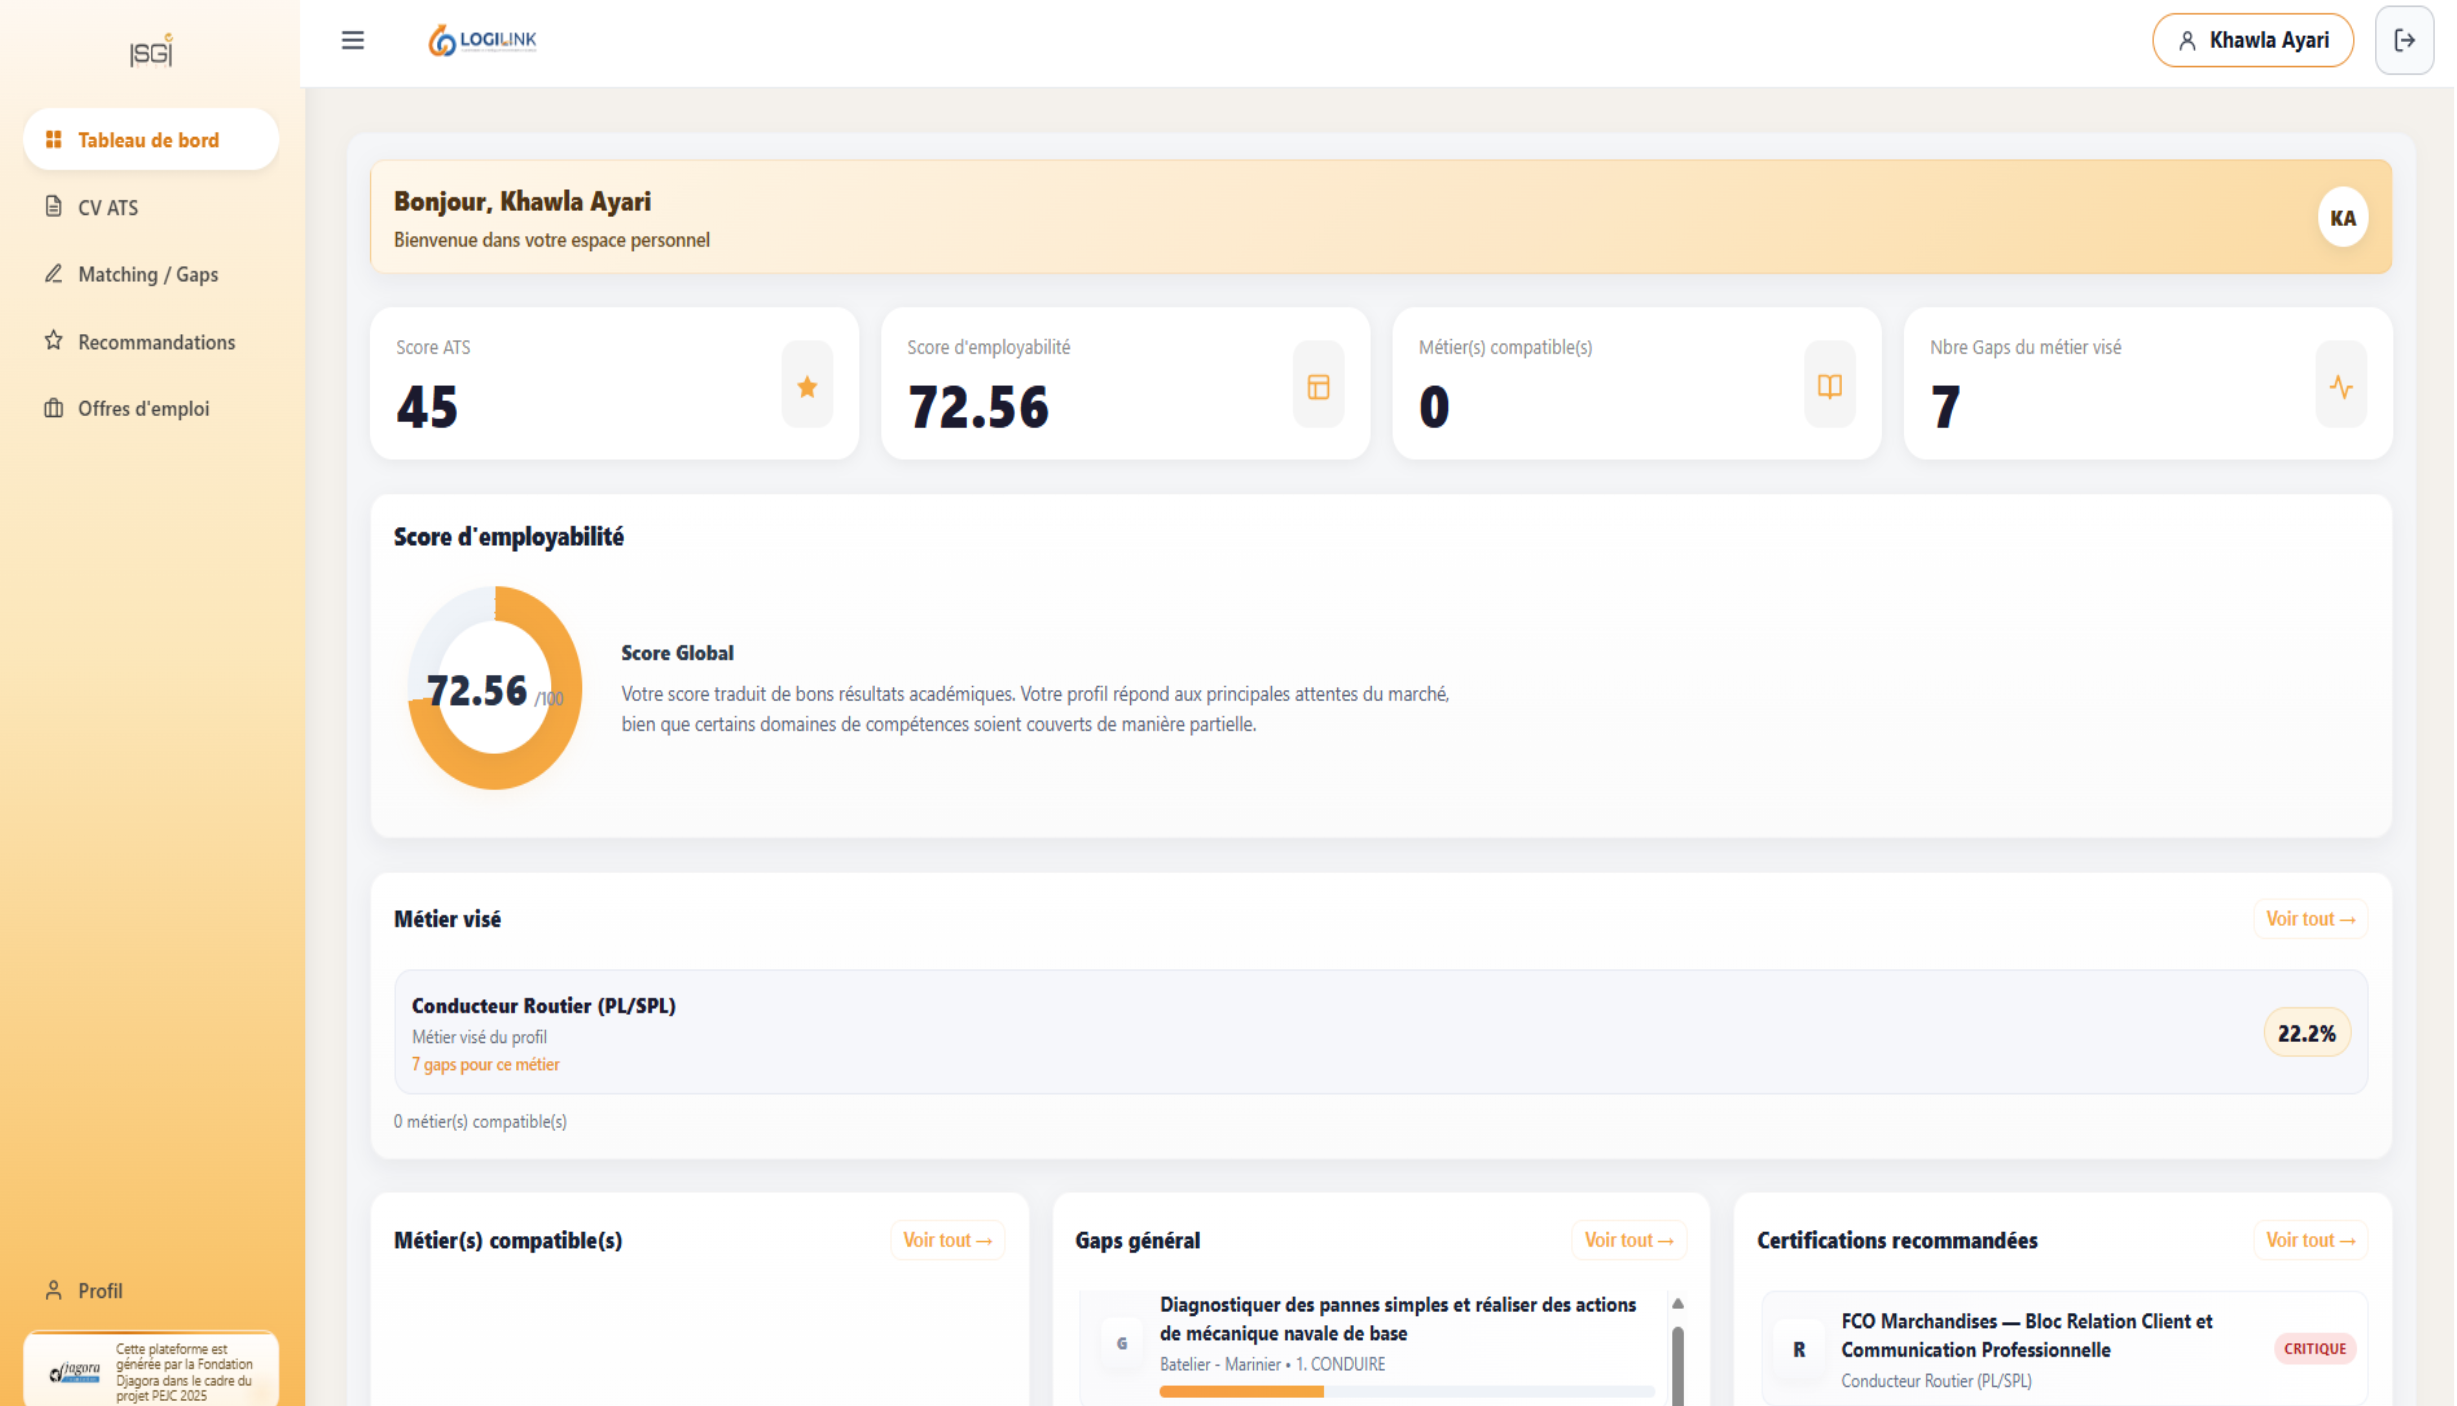
\includegraphics[width=0.85\textwidth]{figures/Interface_du_profil_etudiant.png}
\caption{Interface du profil étudiant}
\label{fig:profil-etudiant}
\end{figure}

\subsubsection{Génération du CV ATS}

La figure~\ref{fig:generation-cv-ats} ci-dessous illustre l'interface de génération du CV ATS, structurée en 11 étapes successives pour garantir un parcours utilisateur fluide. Pour optimiser la saisie, le système intègre un mécanisme d'importation automatique des données institutionnelles de l'ISGIS, pré-remplissant les informations personnelles et extrayant les Hard Skills directement depuis le relevé de notes en fonction du poste visé.
Les autres sections (profil, diplômes, stages, soft skills, langues, projets, certifications et activités para-universitaires) sont complétées manuellement.
De plus, un dispositif de restauration des données permet à l'utilisateur, lors de ses connexions ultérieures, de retrouver et de modifier instantanément ses informations.

\begin{figure}[H]
\centering
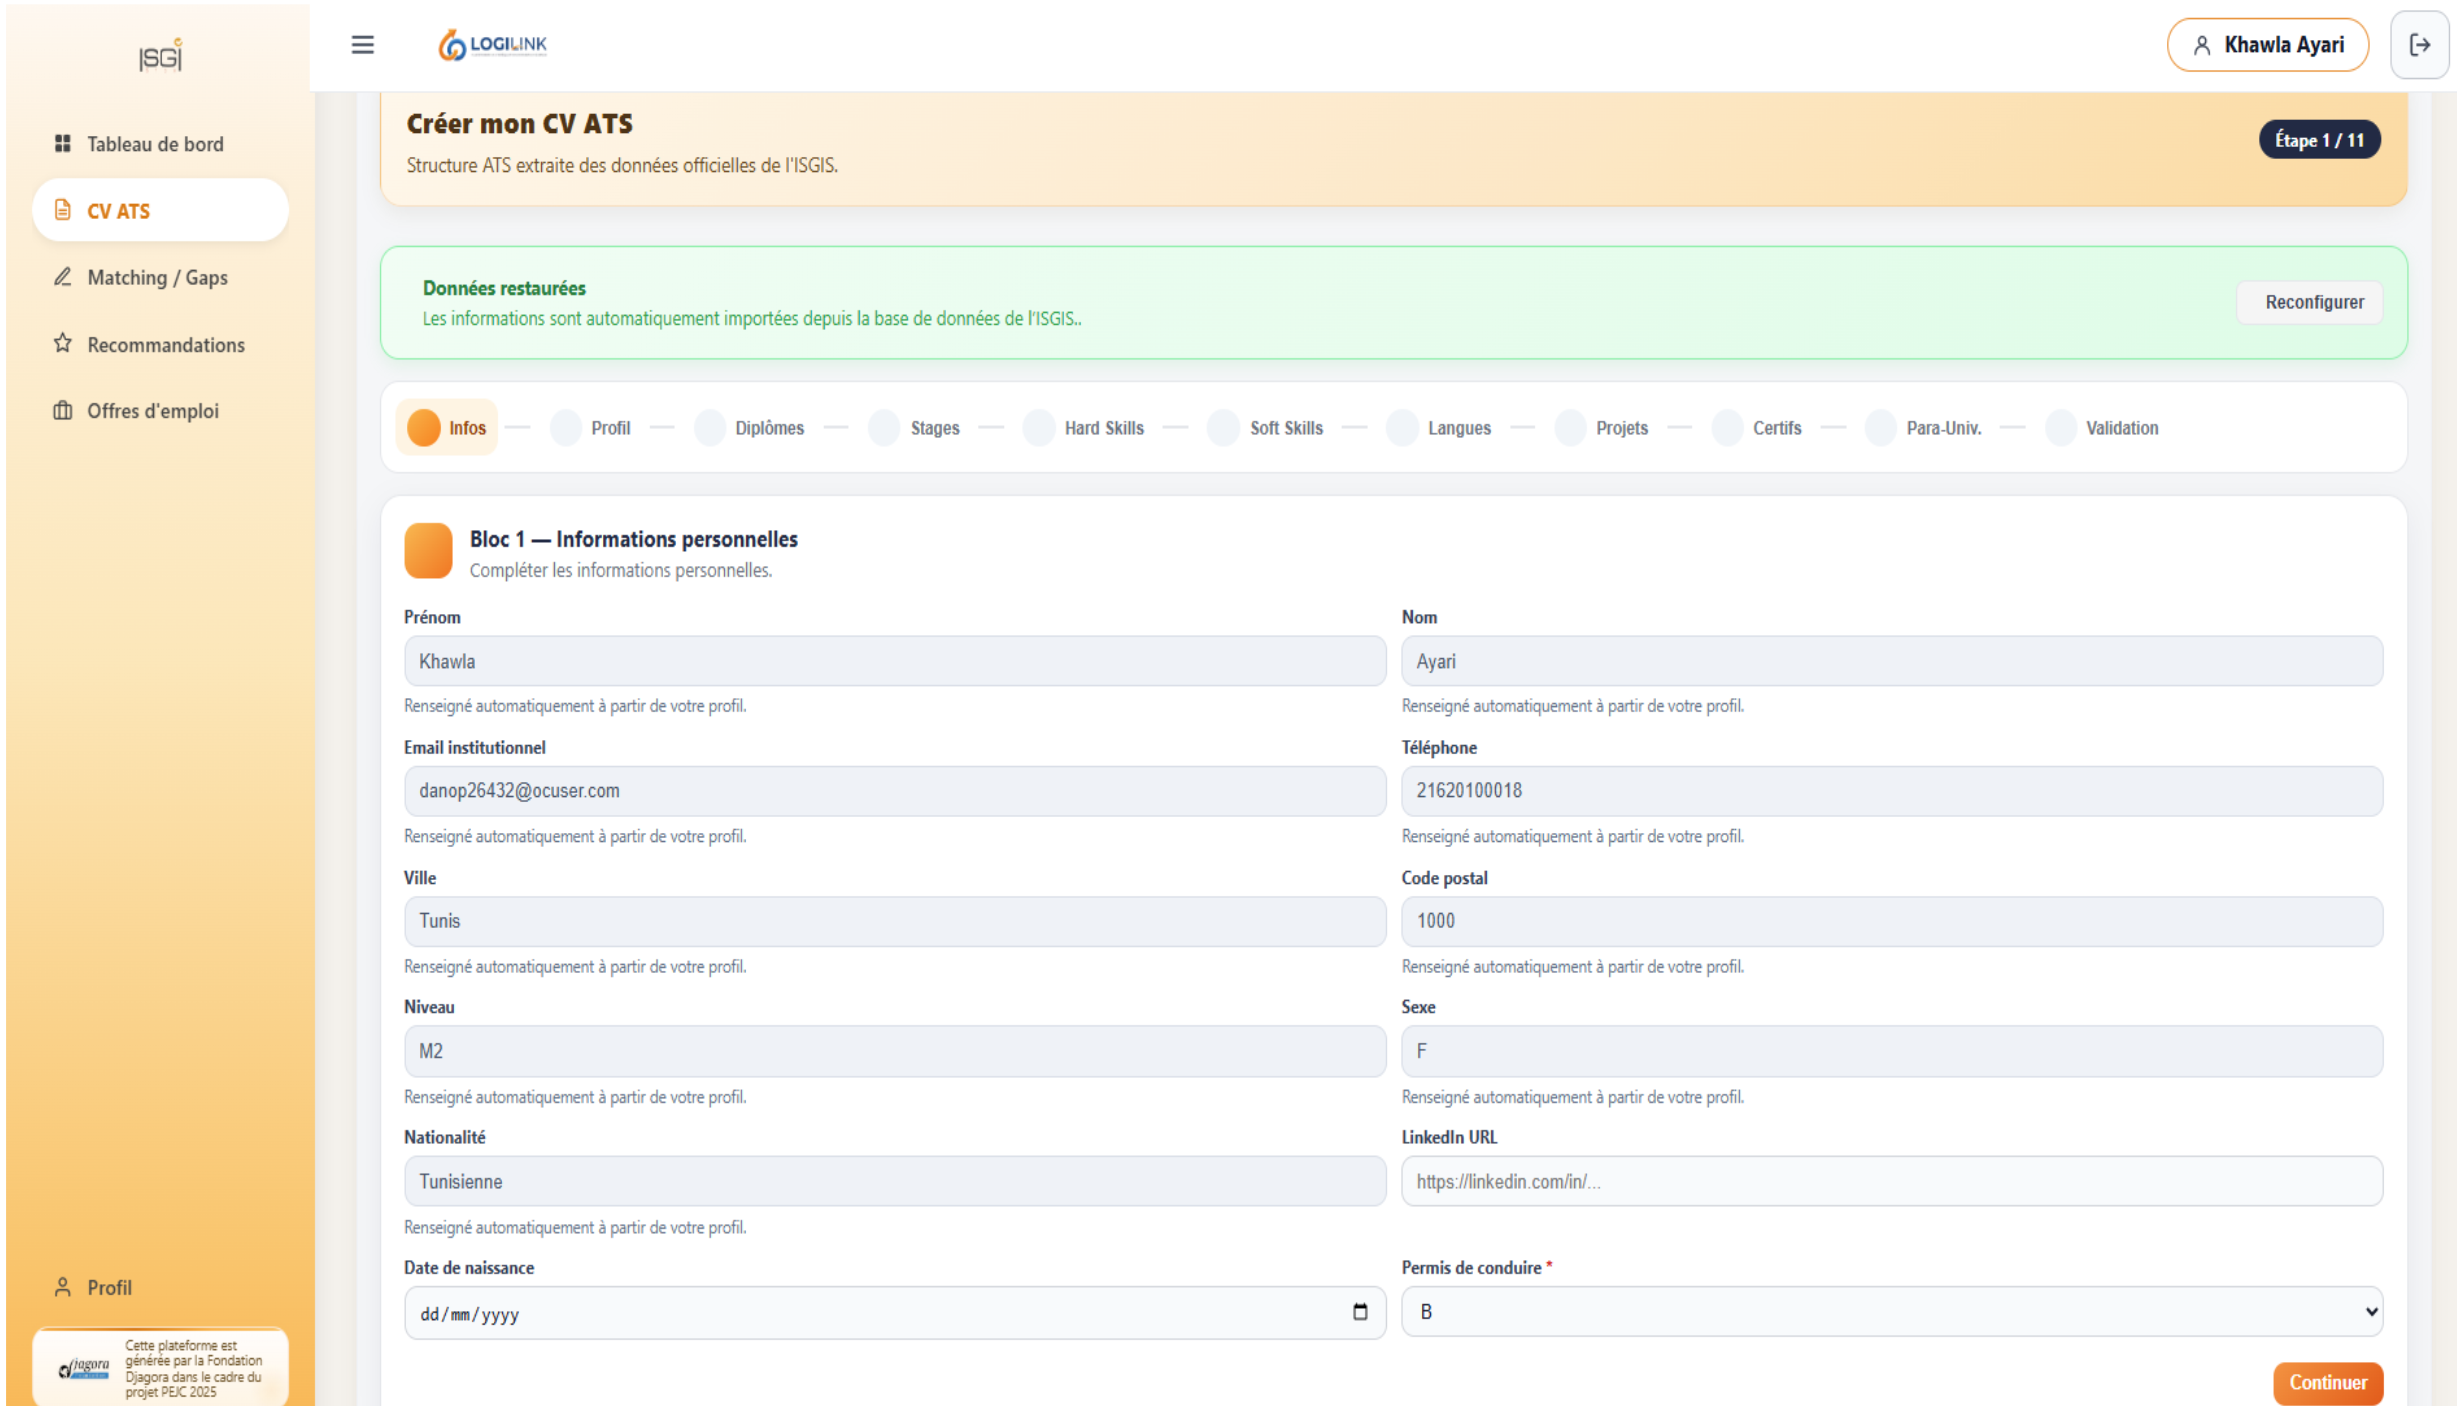
\includegraphics[width=0.85\textwidth]{figures/Interface_de_generation_du_CV_ATS.png}
\caption{Interface de génération du CV ATS}
\label{fig:generation-cv-ats}
\end{figure}

\noindent La figure \ref{fig:validation-cv-ats} présente l'étape finale de validation, qui permet à l'étudiant de vérifier l'ensemble de ses données avant de générer son CV ATS.

\begin{figure}[H]
\centering
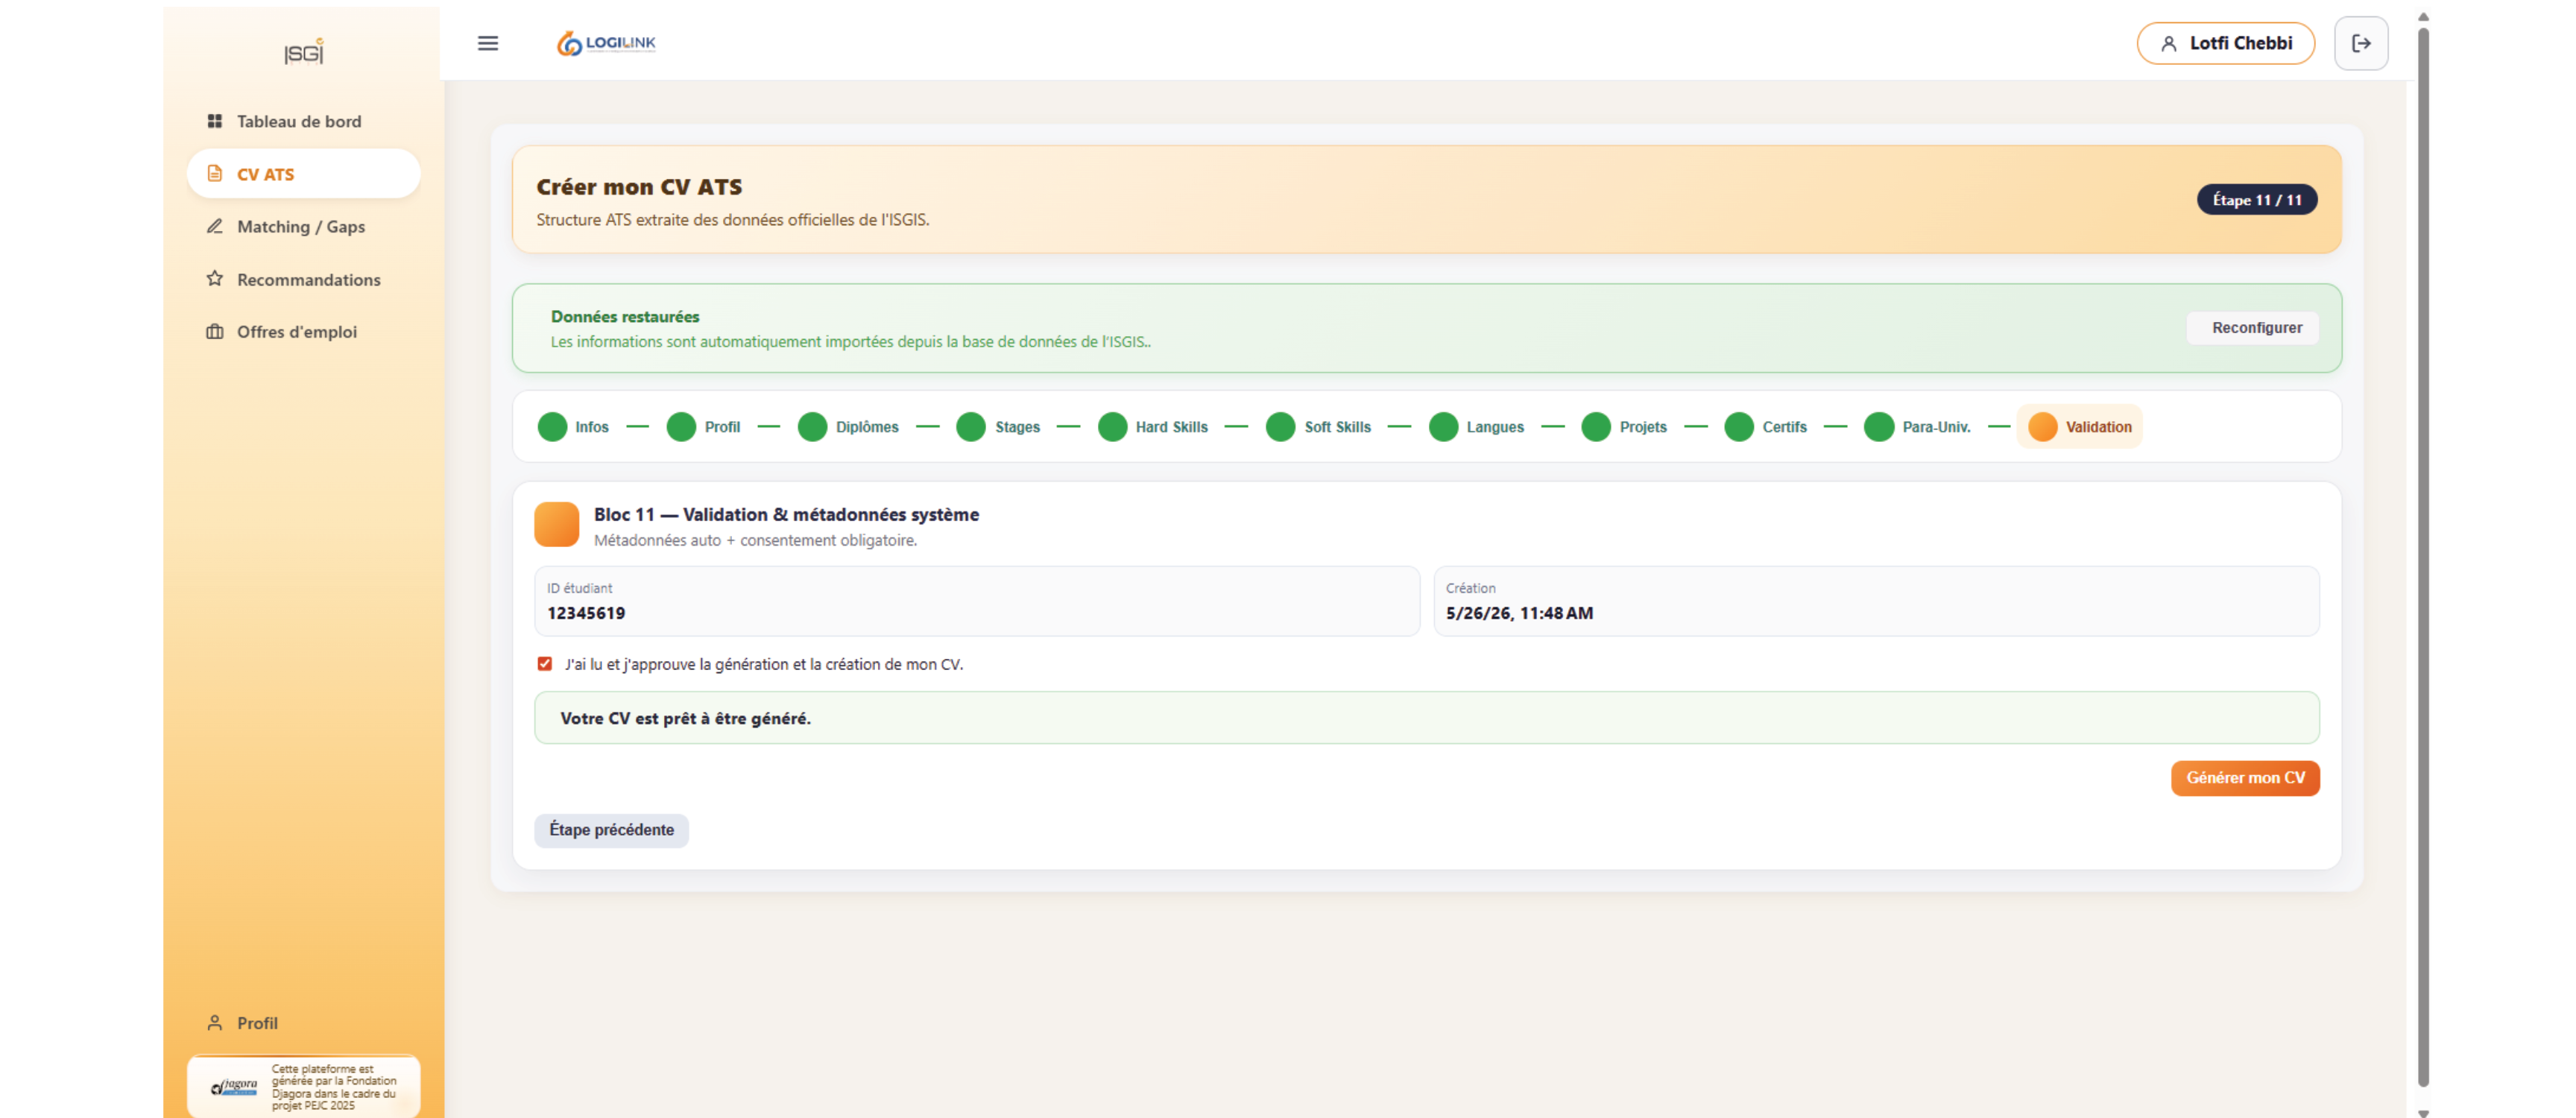
\includegraphics[width=0.85\textwidth]{figures/Interface_de_validation_du_CV_ATS.png}
\caption{Interface de validation du CV ATS}
\label{fig:validation-cv-ats}
\end{figure}

\noindent La figure \ref{fig:cv-ats-genere} illustre le CV généré. Depuis cet espace, l'étudiant a la possibilité de modifier ses informations, de télécharger son document au format PDF et de cliquer sur le bouton "Évaluer votre CV" afin de stocker le CV, lancer le calcul de ses scores ATS et d'employabilité.

\begin{figure}[H]
\centering
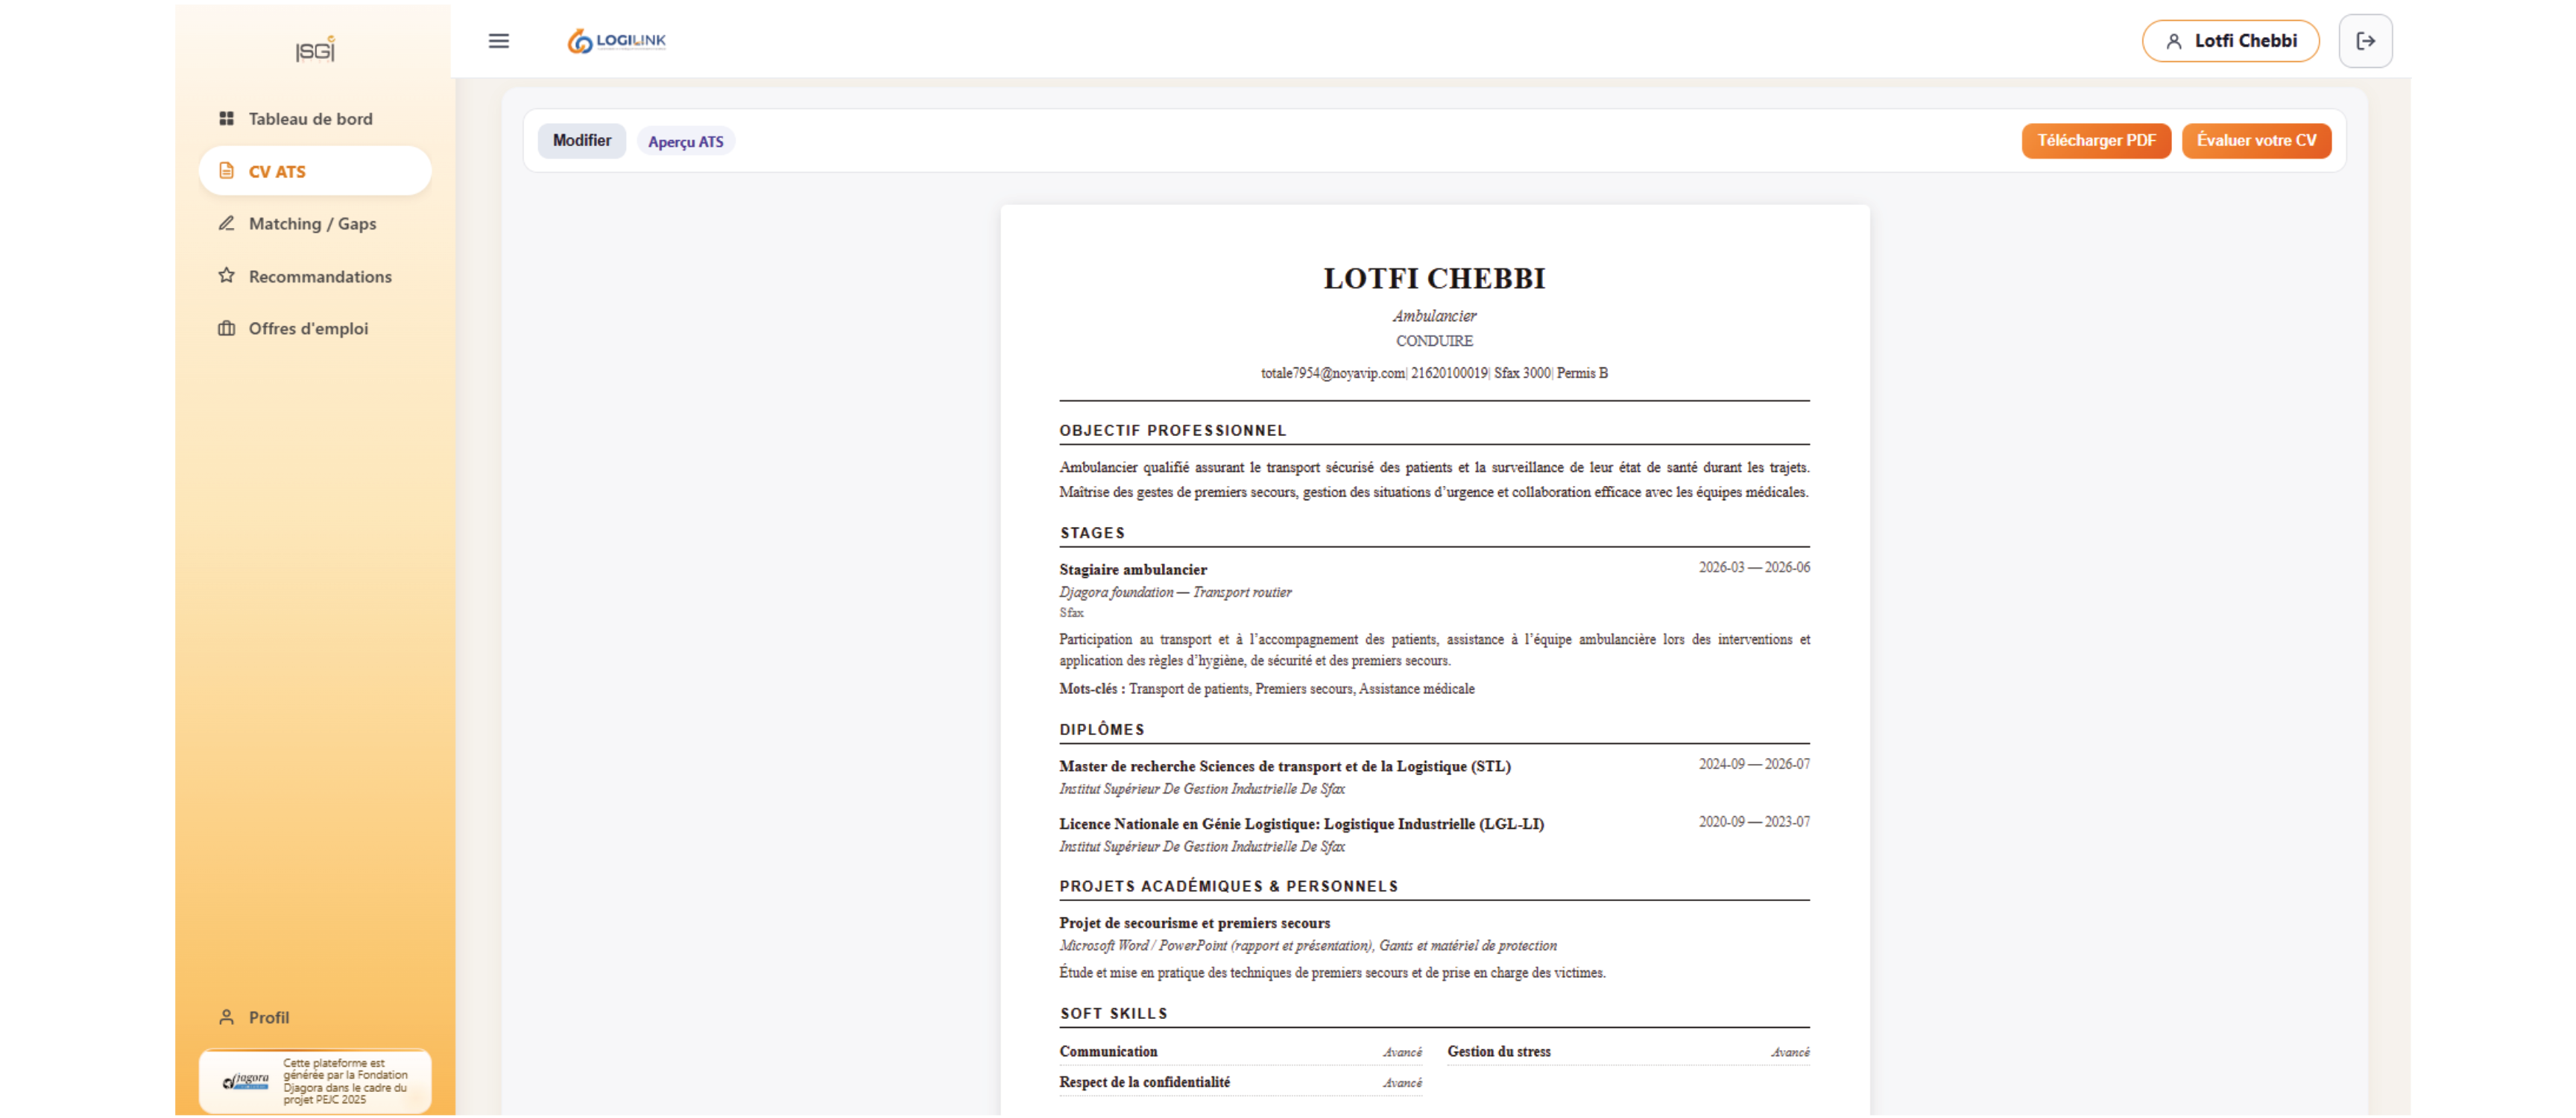
\includegraphics[width=0.85\textwidth]{figures/Interface_du_CV_ATS_genere.png}
\caption{Interface du CV ATS généré}
\label{fig:cv-ats-genere}
\end{figure}

\subsubsection{Calcul du score ats et employabilité}

La figure \ref{fig:tableau-bord-etudiant} ci-dessous présente le tableau de bord principal de l'étudiant. Cet espace regroupe les résultats d'analyse de la plateforme et affiche les scores ATS et d'employabilité.

\begin{figure}[H]
\centering
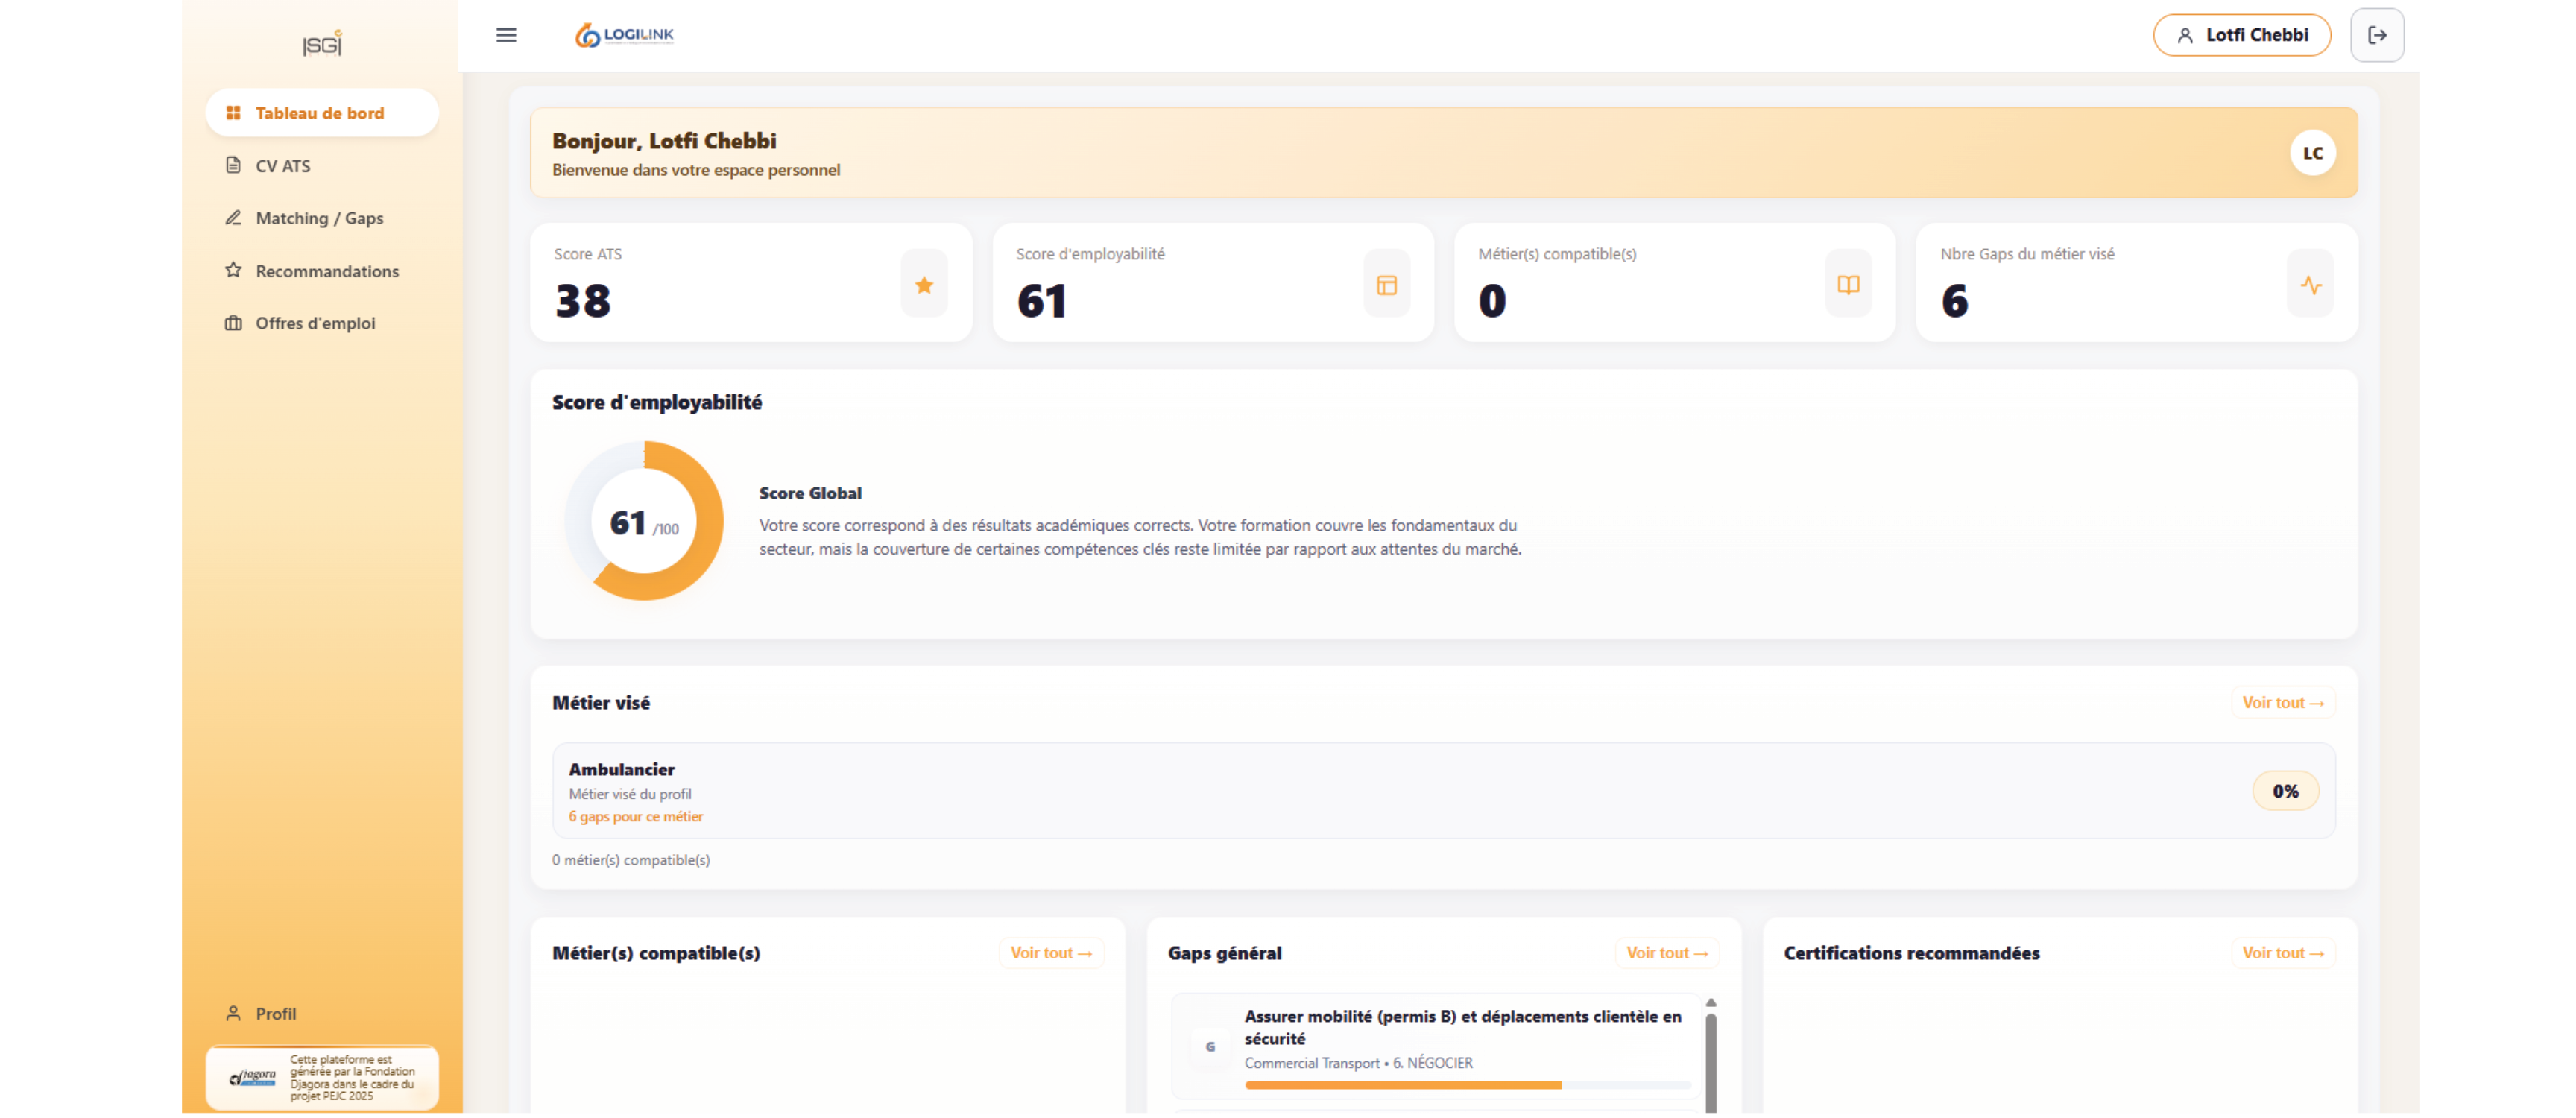
\includegraphics[width=0.85\textwidth]{figures/Interface_du_tableau_de_bord_de_laetudiant.png}
\caption{Interface du tableau de bord de l'étudiant}
\label{fig:tableau-bord-etudiant}
\end{figure}

\subsubsection{Calcul du score d'employabilité prévisionnel}

\noindent La figure~\ref{fig:prediction-score-employabilite} suivante montre que lorsque l'étudiant clique sur le bouton "Prédire votre nouveau score", un score d'employabilité prévisionnel est automatiquement généré en tenant compte des recommandations obtenues.

\begin{figure}[H]
\centering
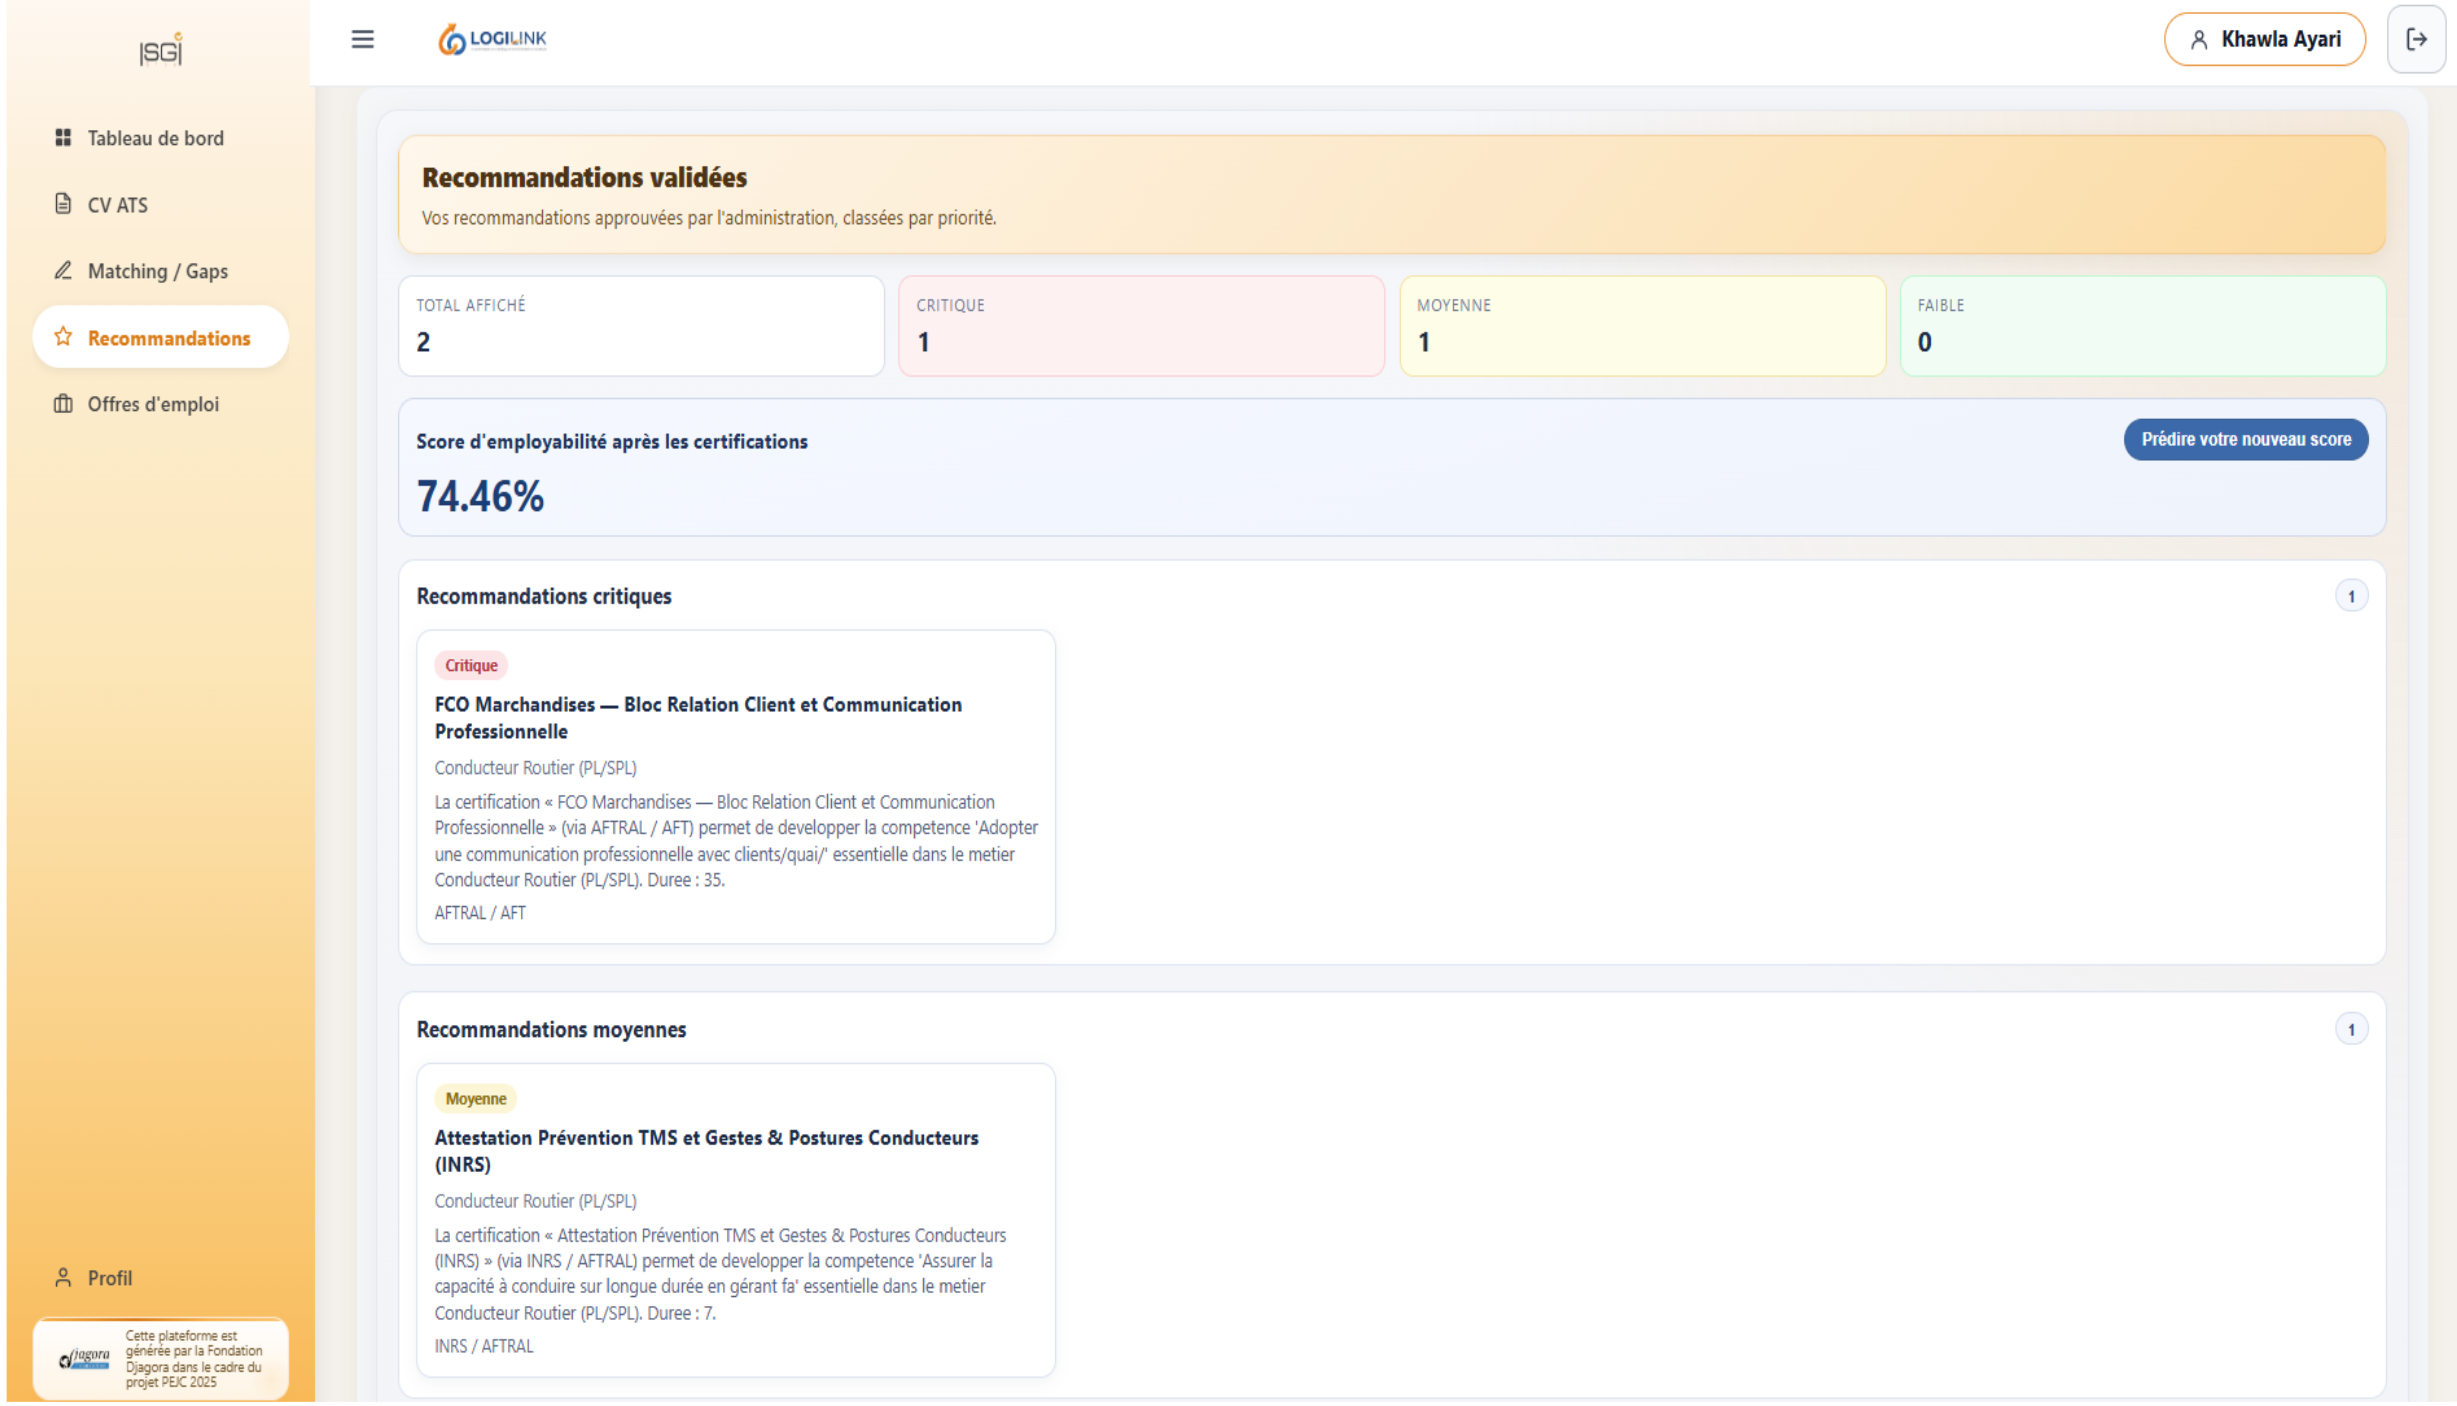
\includegraphics[width=0.85\textwidth]{figures/Interface_de_prediction_du_score_daemployabilite.png}
\caption{Interface de prédiction du score d'employabilité}
\label{fig:prediction-score-employabilite}
\end{figure}

\subsection{Interfaces admin}

\noindent Les figures~\ref{fig:tableau-bord-admin}~et~\ref{fig:tableau-bord-admin-2} ci-dessous présentent le tableau de bord de l'administrateur, un espace de pilotage centralisant les indicateurs clés ainsi que des graphiques d'analyse. Elle permet de visualiser la répartition des étudiants par filière, d'observer la distribution des scores ATS et des scores d'employabilité, et de consulter une liste des étudiants les mieux classés selon le score d'employabilité.

\begin{figure}[H]
\centering
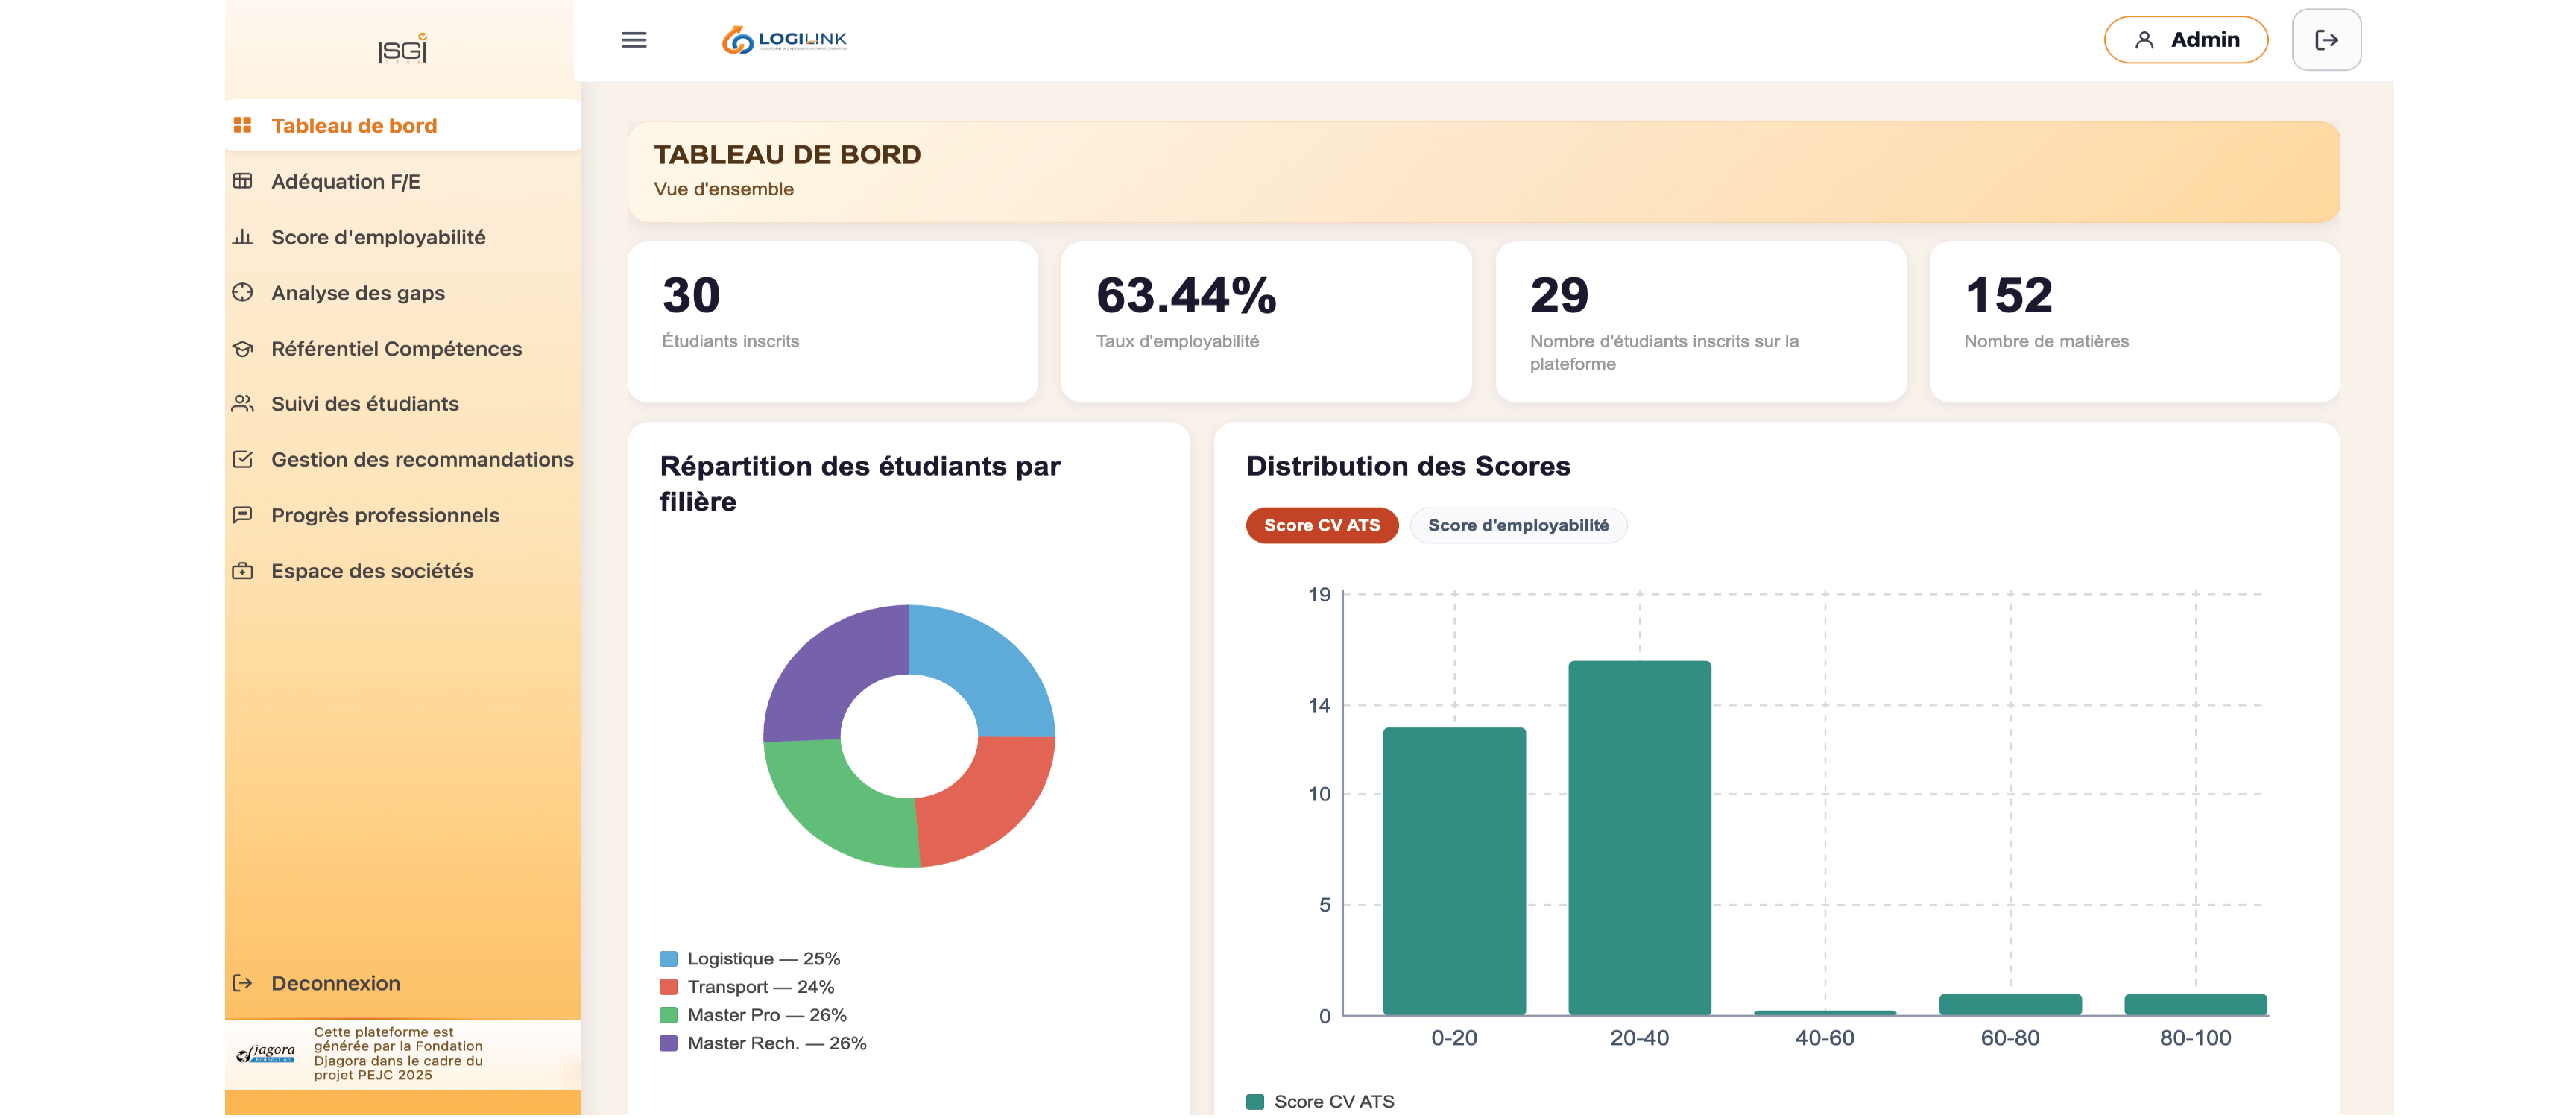
\includegraphics[width=0.85\textwidth]{figures/Interface_du_tableau_de_bord_de_laadministrateur.png}
\caption{Interface du tableau de bord de l'administrateur}
\label{fig:tableau-bord-admin}
\end{figure}

\begin{figure}[H]
\centering
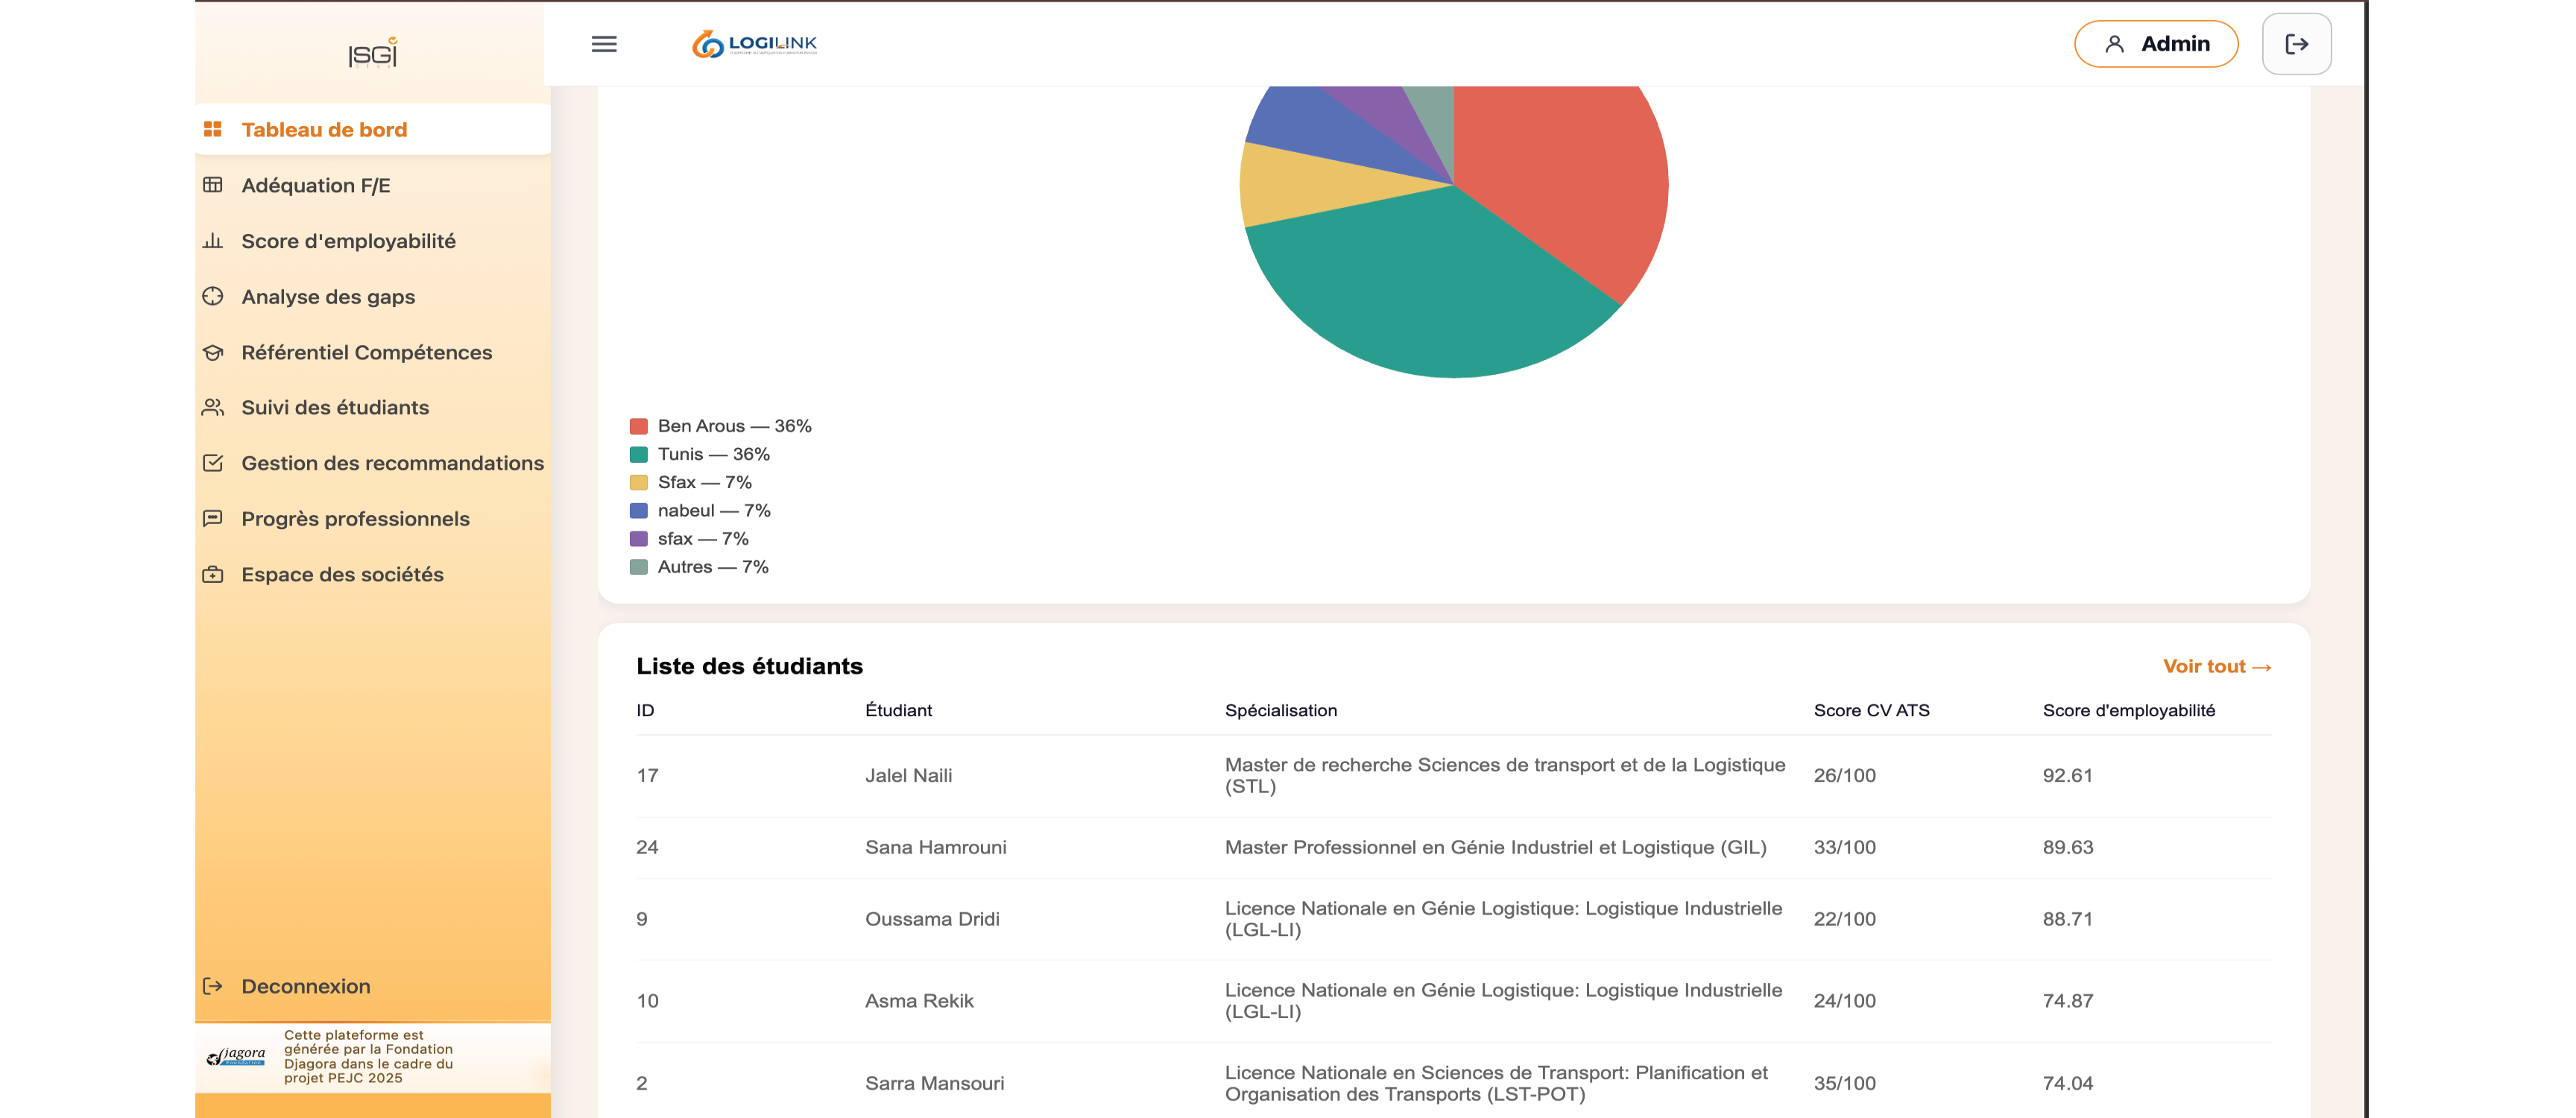
\includegraphics[width=0.85\textwidth]{figures/Interface_du_tableau_de_bord_de_laadministrateur_2.png}
\caption{Interface du tableau de bord de l'administrateur}
\label{fig:tableau-bord-admin-2}
\end{figure}

\noindent Les figures~\ref{fig:score-employabilite}~et~\ref{fig:score-employabilite-2} ci-dessous illustrent l'interface Score d'employabilité. Elle présente le nombre d'étudiants inscrits, le nombre d'étudiants classés parmi les meilleurs profils, ainsi que le score global d'employabilité. L'interface propose ensuite la distribution des scores, une analyse par filière et une comparaison par type de parcours (Licence, Master, Licence + Master).

\begin{figure}[H]
\centering
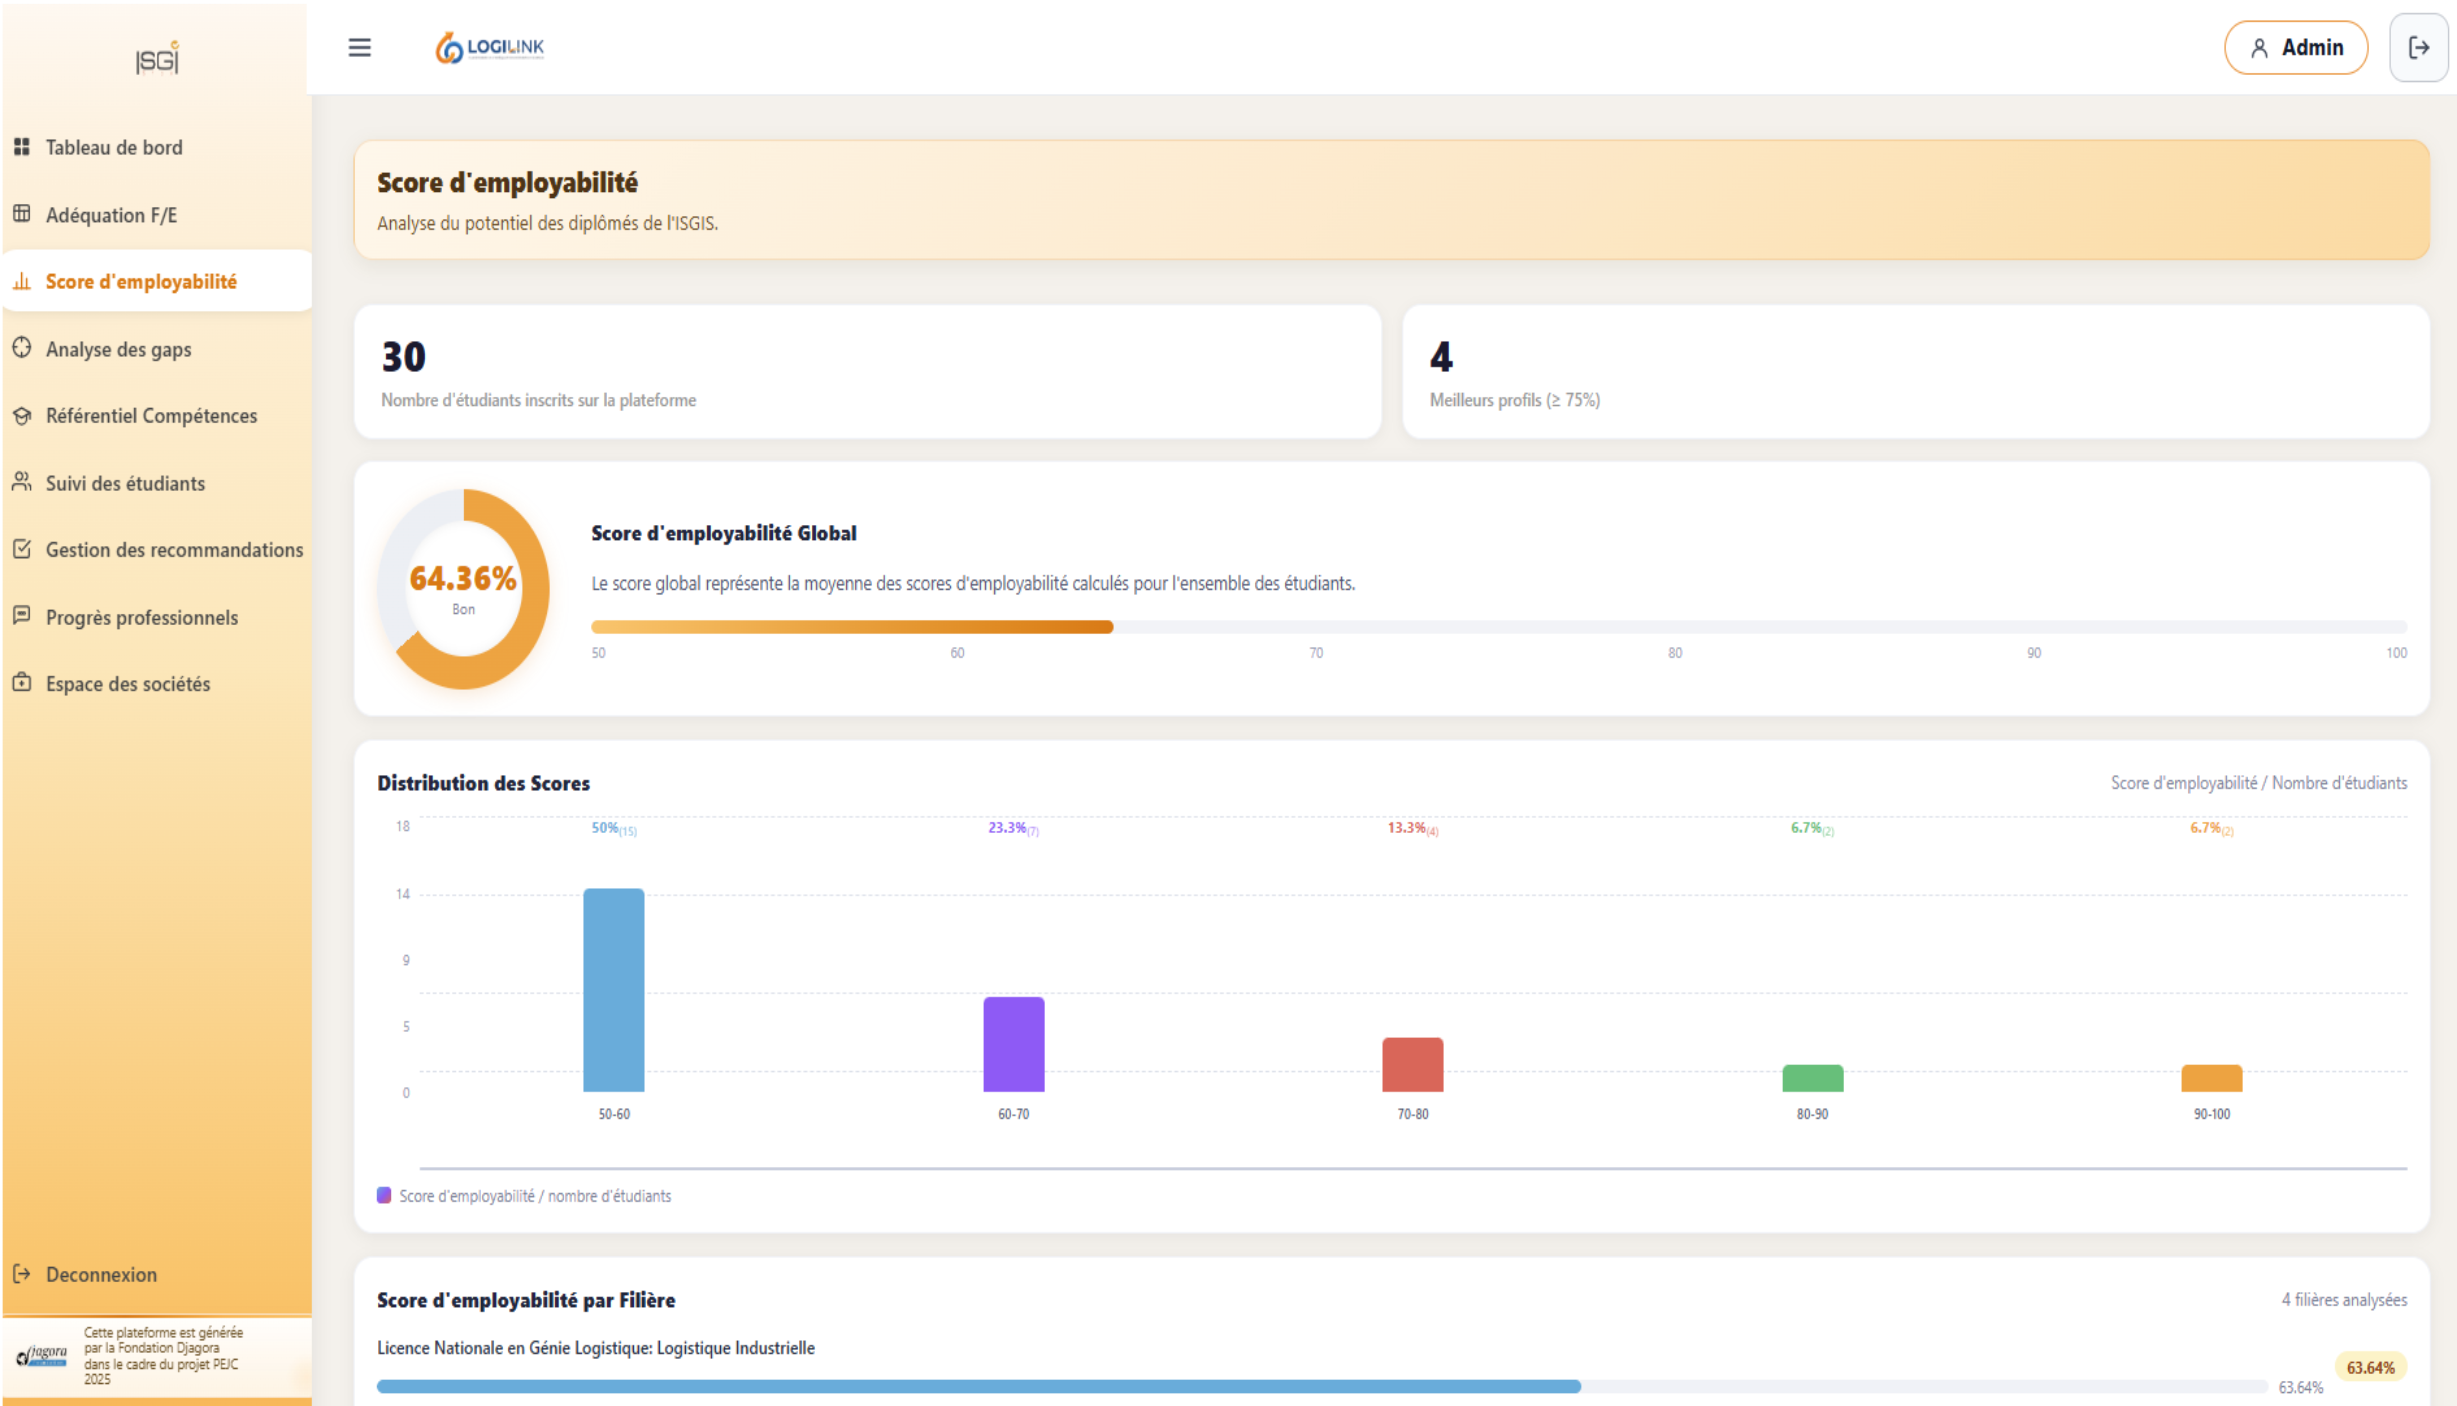
\includegraphics[width=0.85\textwidth]{figures/Interface_du_score_daemployabilite.png}
\caption{Interface du score d'employabilité}
\label{fig:score-employabilite}
\end{figure}

\begin{figure}[H]
\centering
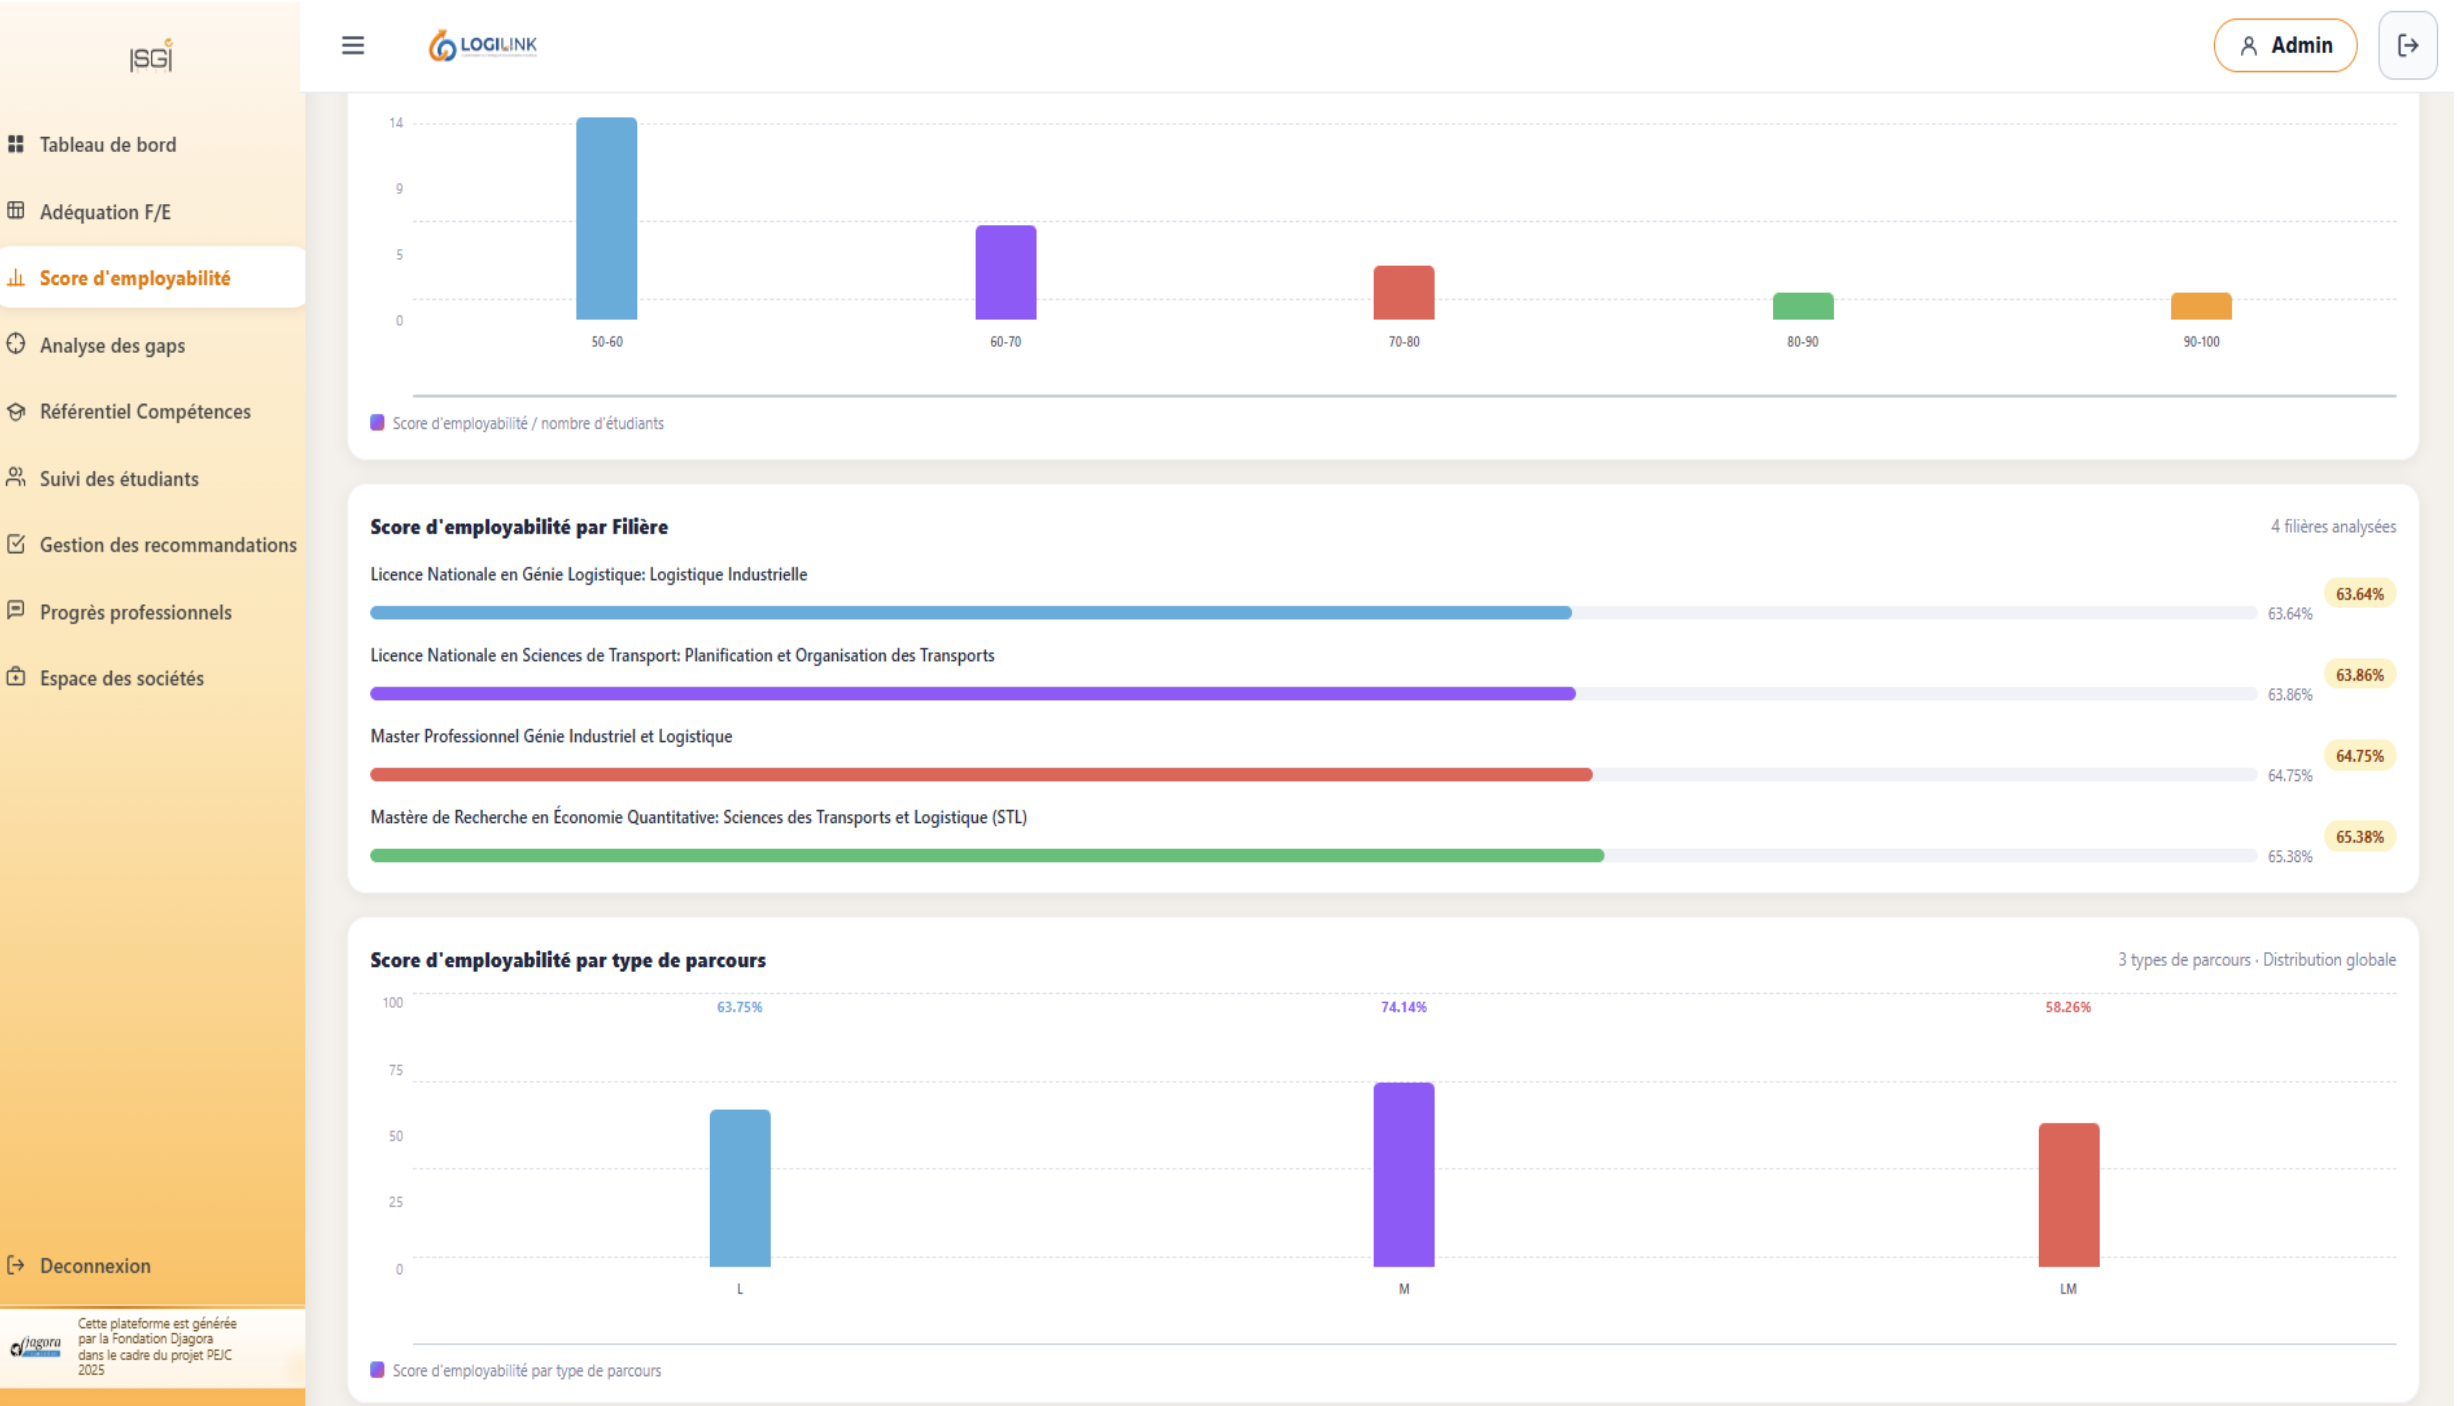
\includegraphics[width=0.85\textwidth]{figures/Interface_du_score_daemployabilite_2.png}
\caption{Interface du score d'employabilité}
\label{fig:score-employabilite-2}
\end{figure}

\noindent La figure~\ref{fig:adequation-formation-emploi} ci-dessous présente l'interface d'adéquation Formation-Emploi, qui permet d'analyser la correspondance entre les matières enseignées et les métiers. Elle intègre une matrice de couverture des compétences pouvant être filtrée par parcours et par filière. Chaque cellule de la matrice est associée à un coefficient variant de 0 à 1 (0 ; 0,2 ; 0,4 ; 0,6 ; 0,8 ; 1), indiquant le niveau de contribution de la matière au métier concerné.

\begin{figure}[H]
\centering
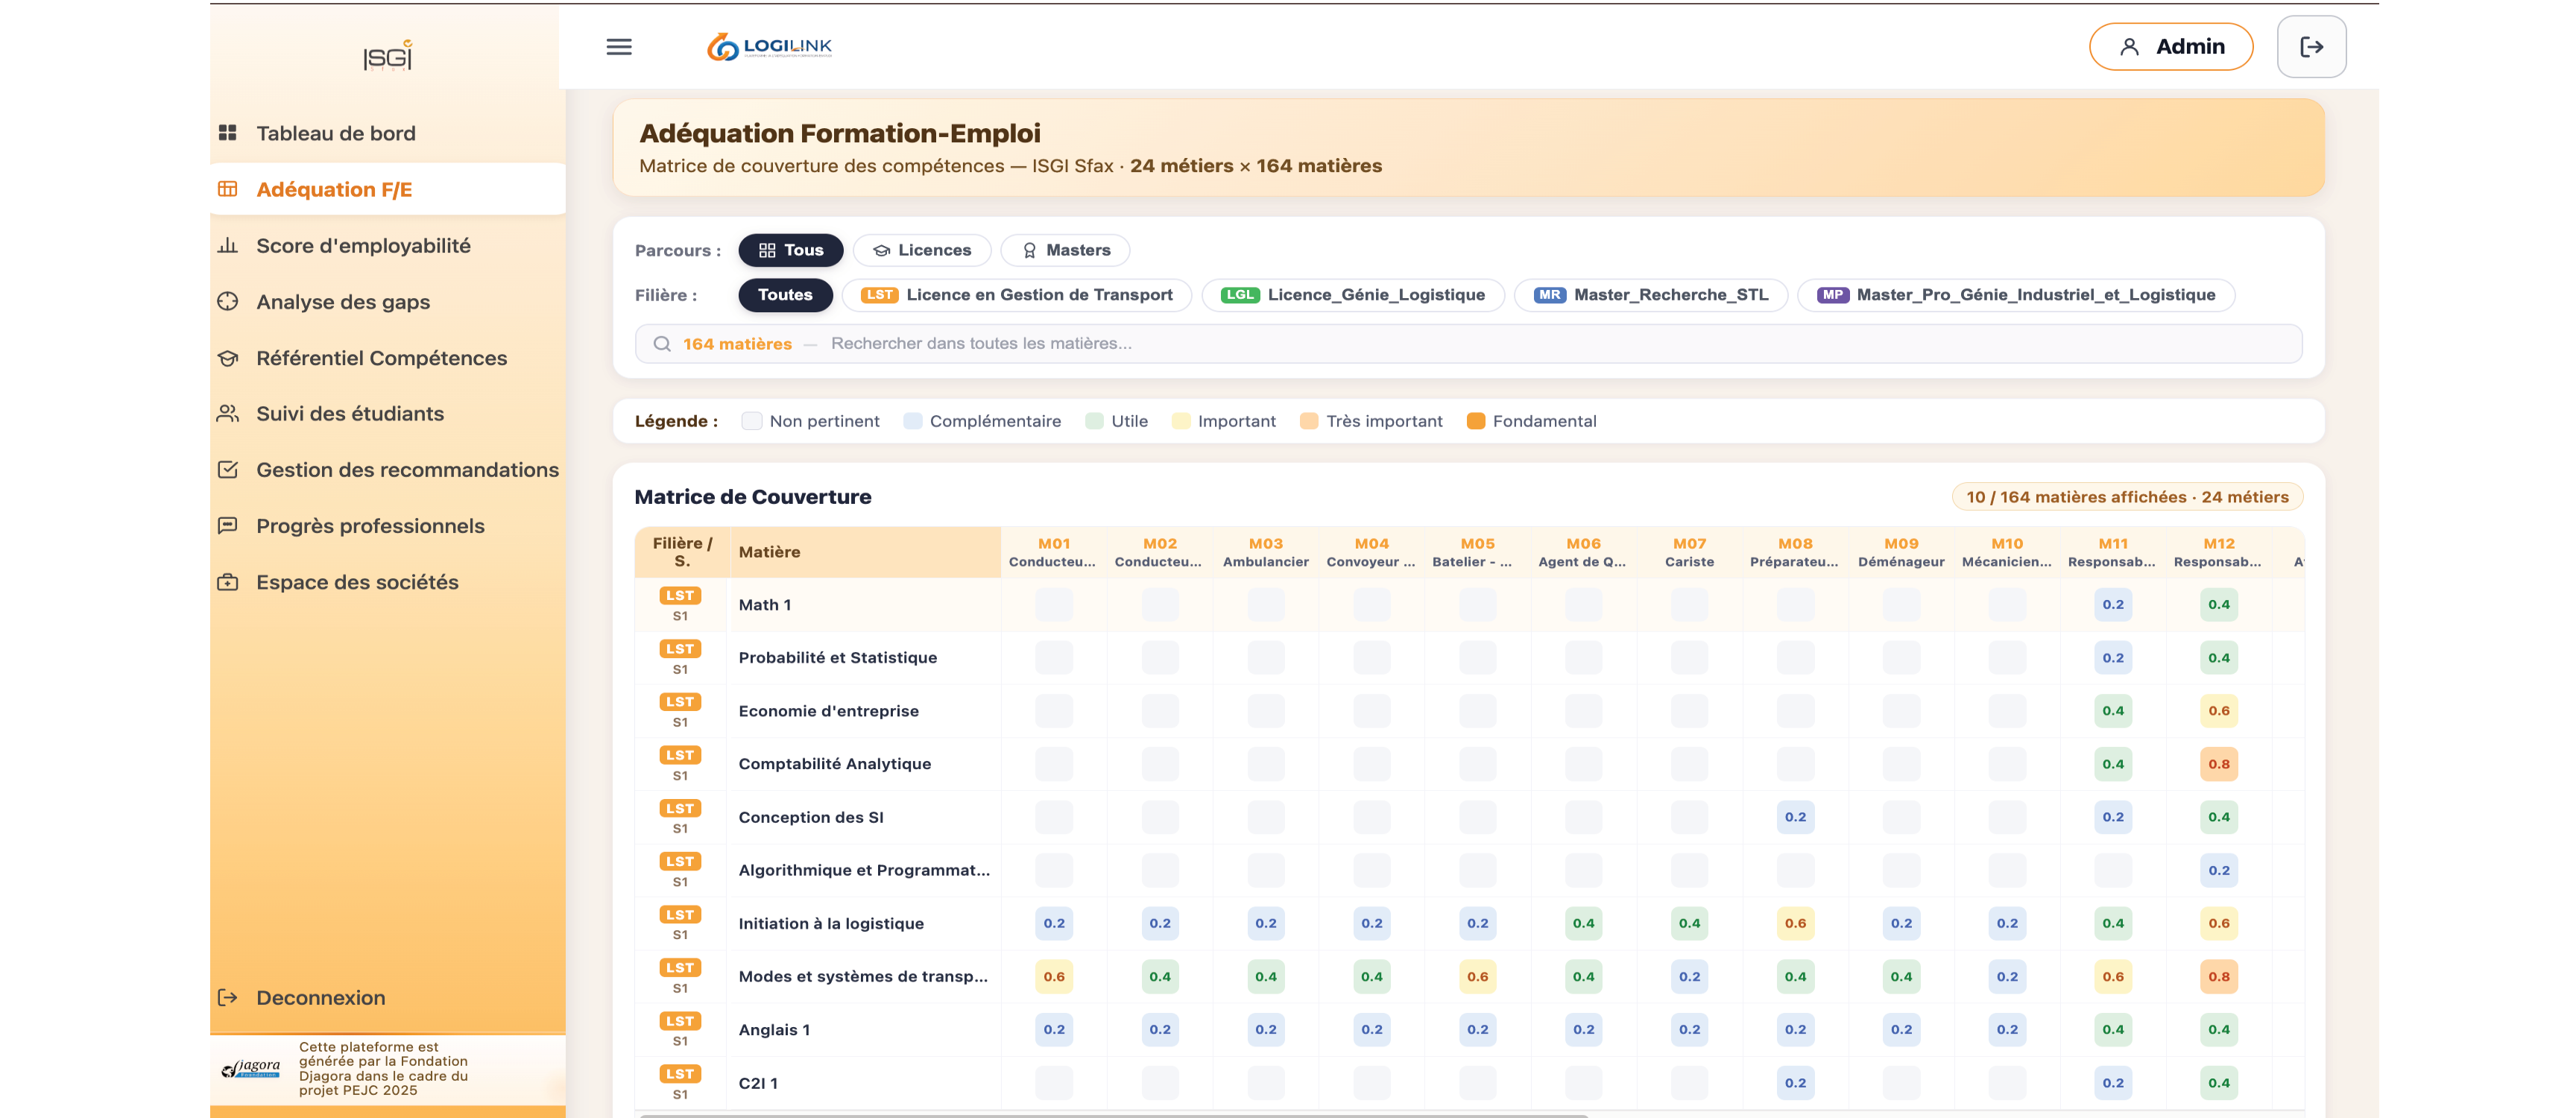
\includegraphics[width=0.85\textwidth]{figures/Interface_daadequation_Formation-Emploi.png}
\caption{Interface d'adéquation Formation-Emploi}
\label{fig:adequation-formation-emploi}
\end{figure}

\noindent La figure~\ref{fig:referentiel-competences} ci-dessous présente l'interface Référentiel Compétences, qui englobe l'ensemble des compétences par métiers dans le secteur Transport \& Logistique. Ces compétences sont classées par catégorie (techniques, organisationnelles, physiques et comportementales) ainsi que par domaine.

\begin{figure}[H]
\centering
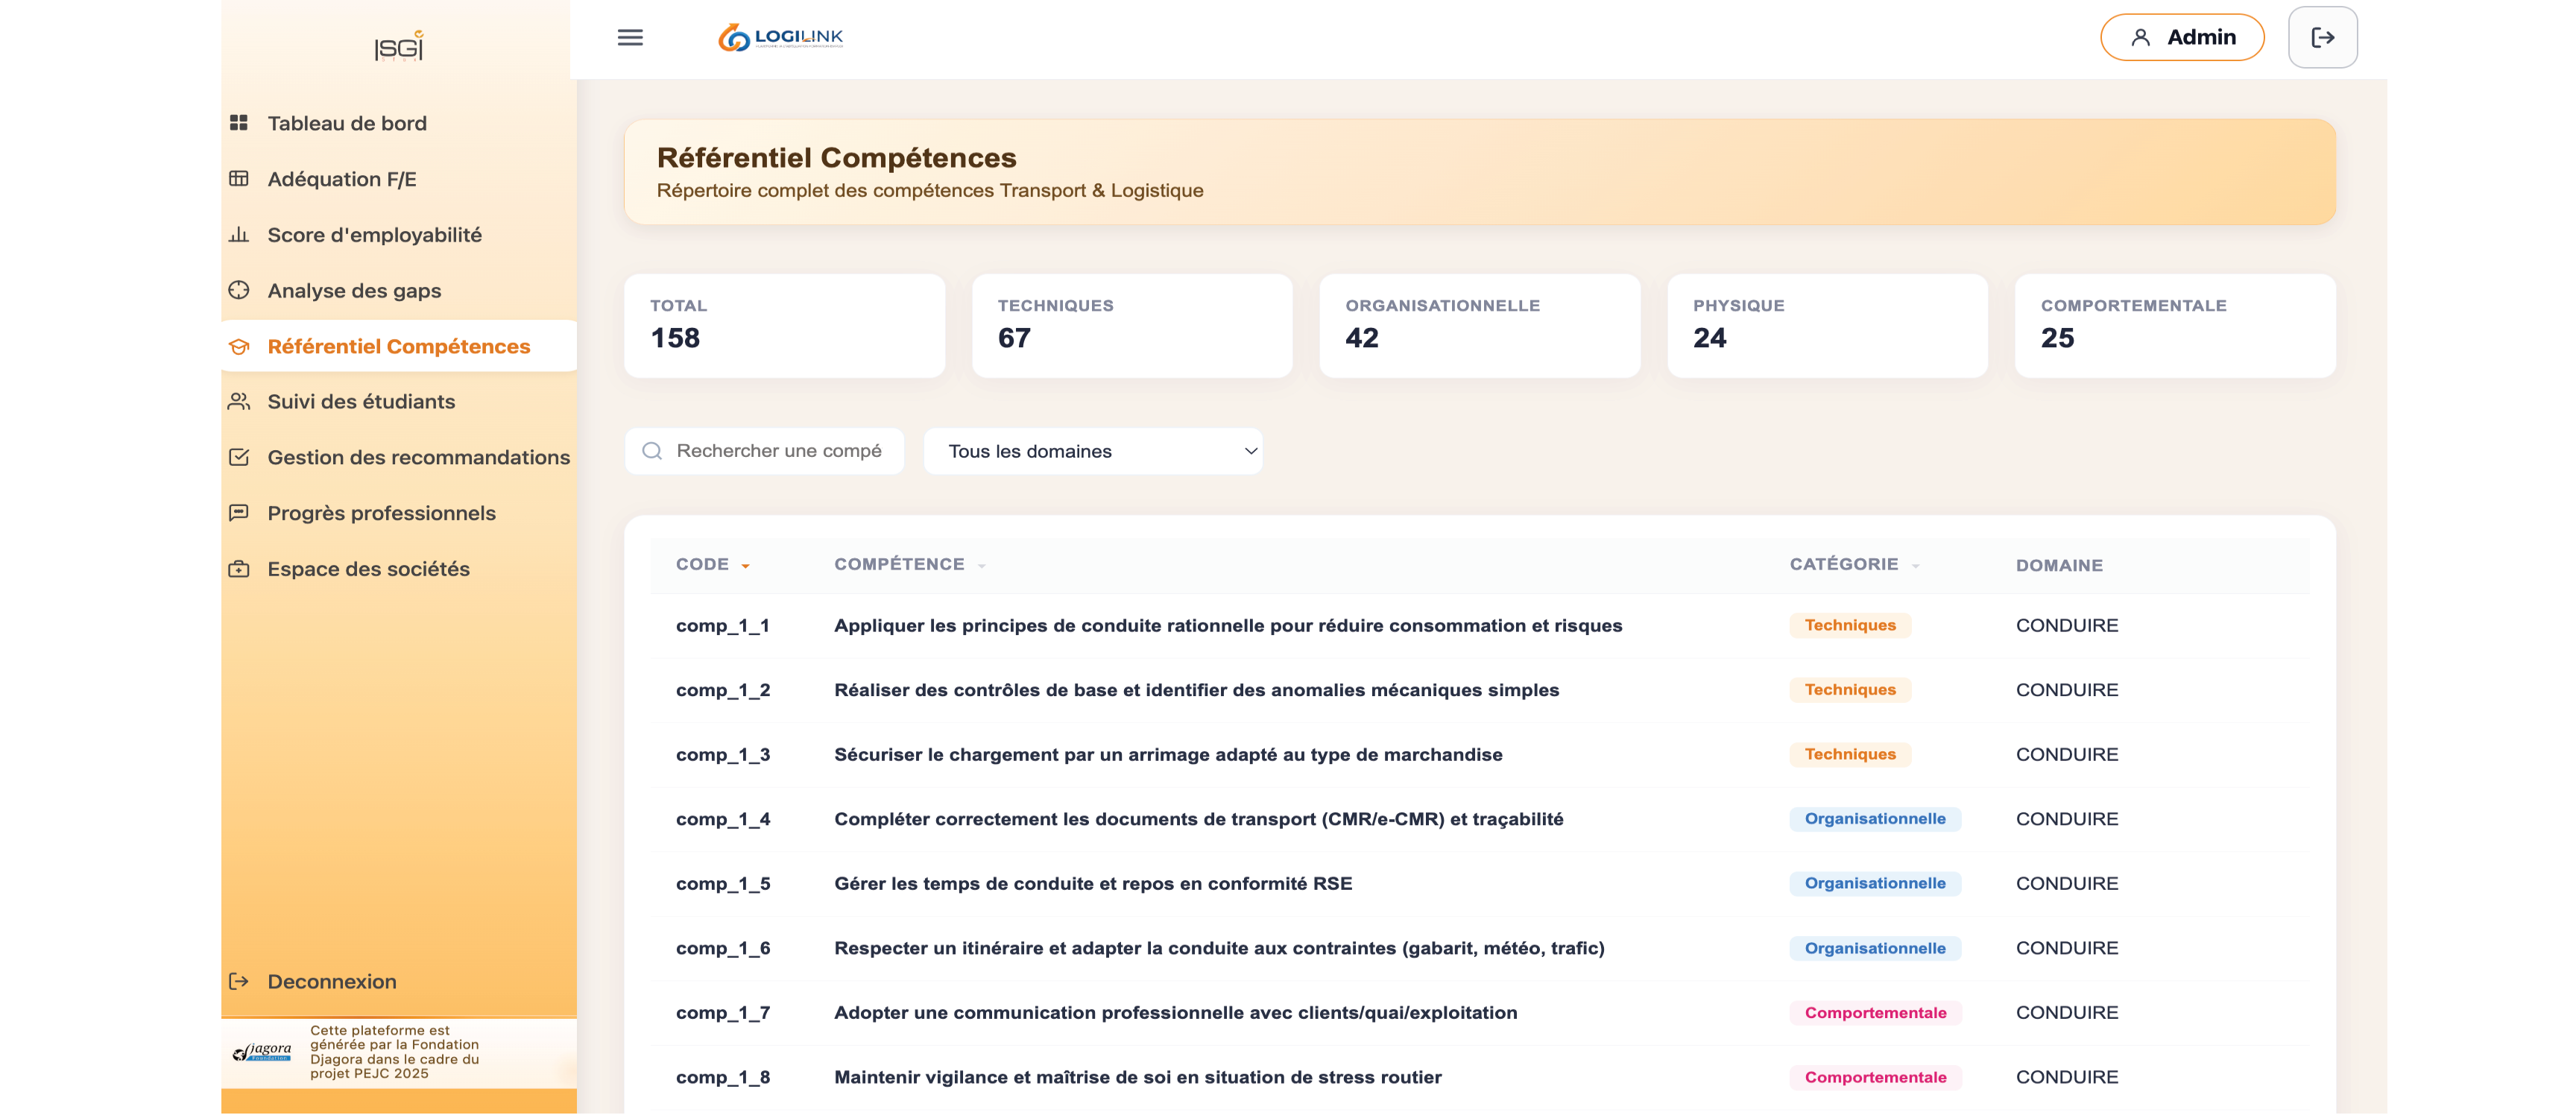
\includegraphics[width=0.85\textwidth]{figures/Interface_du_referentiel_des_competences.png}
\caption{Interface du référentiel des compétences}
\label{fig:referentiel-competences}
\end{figure}

\noindent La figure~\ref{fig:suivi-etudiants-filiere} ci-dessous présente l'interface Suivi des étudiants, ainsi que leur score CV ATS et leur score d'employabilité.

\begin{figure}[H]
\centering
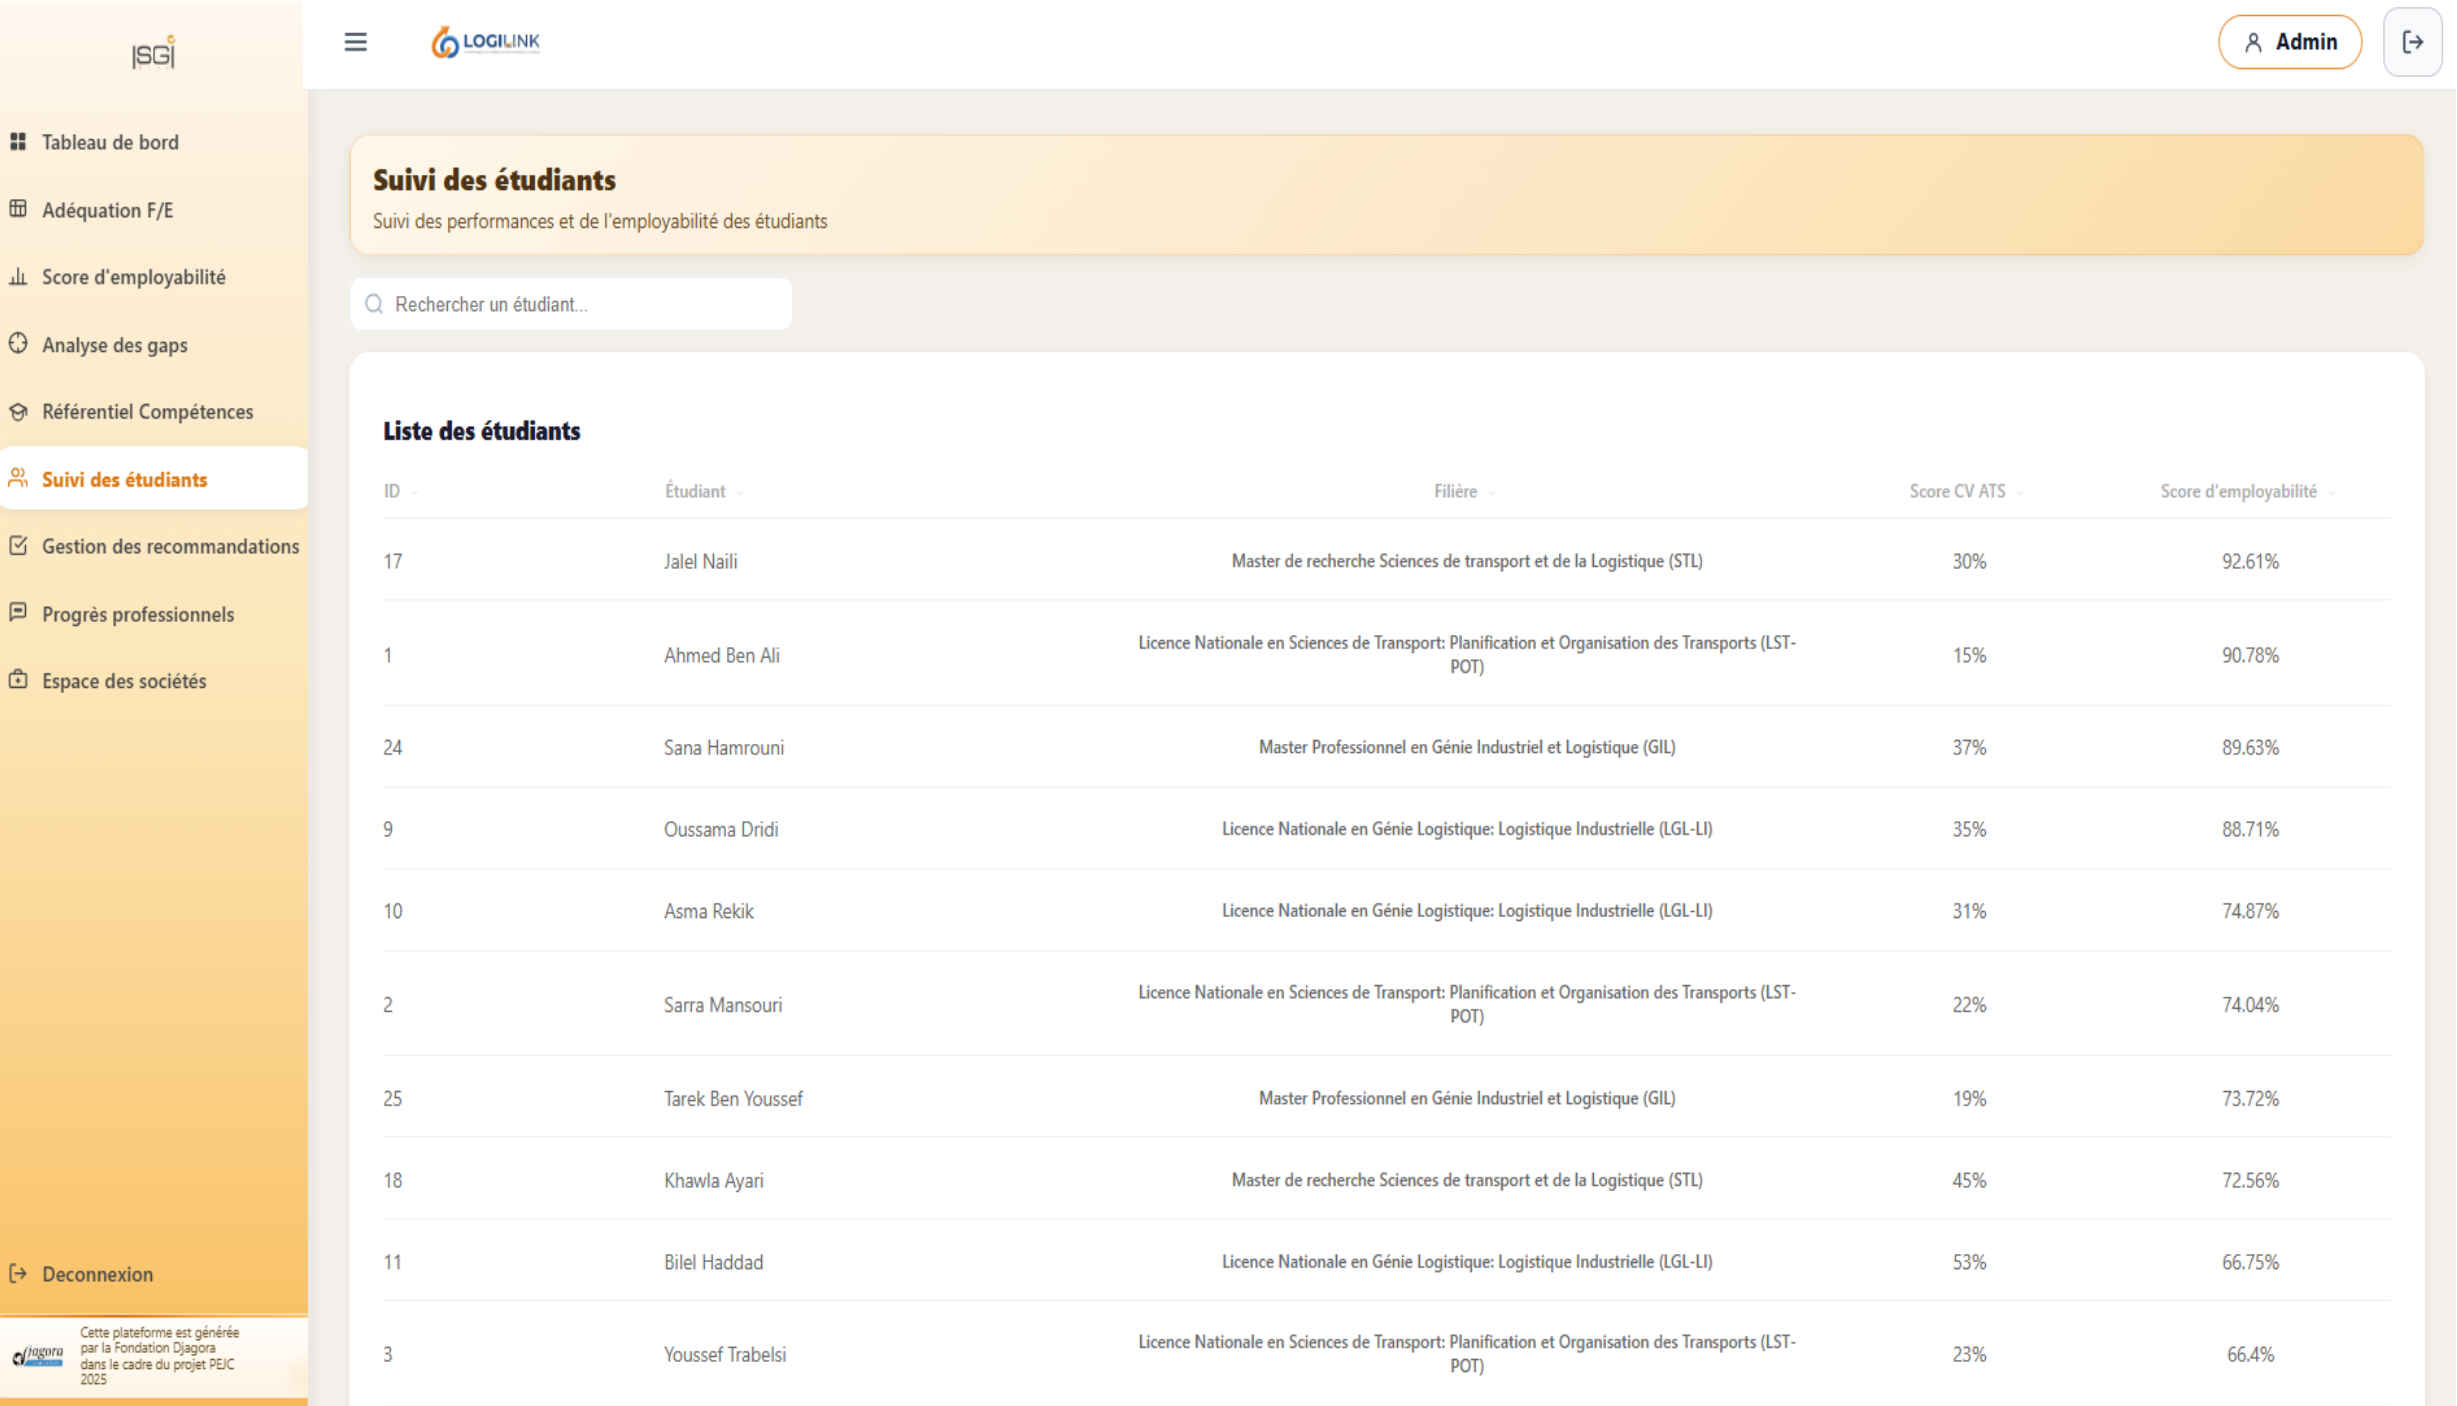
\includegraphics[width=0.85\textwidth]{figures/Interface_de_suivi_des_etudiants_par_filiere.png}
\caption{Interface de suivi des étudiants par filière}
\label{fig:suivi-etudiants-filiere}
\end{figure}

\subsection{Interfaces société}

La figure~\ref{fig:consultation-candidatures} ci-dessous permet à la société de consulter le score d'employabilité ainsi que le CV ATS de l'étudiant ayant postulé à une offre.

\begin{figure}[H]
\centering
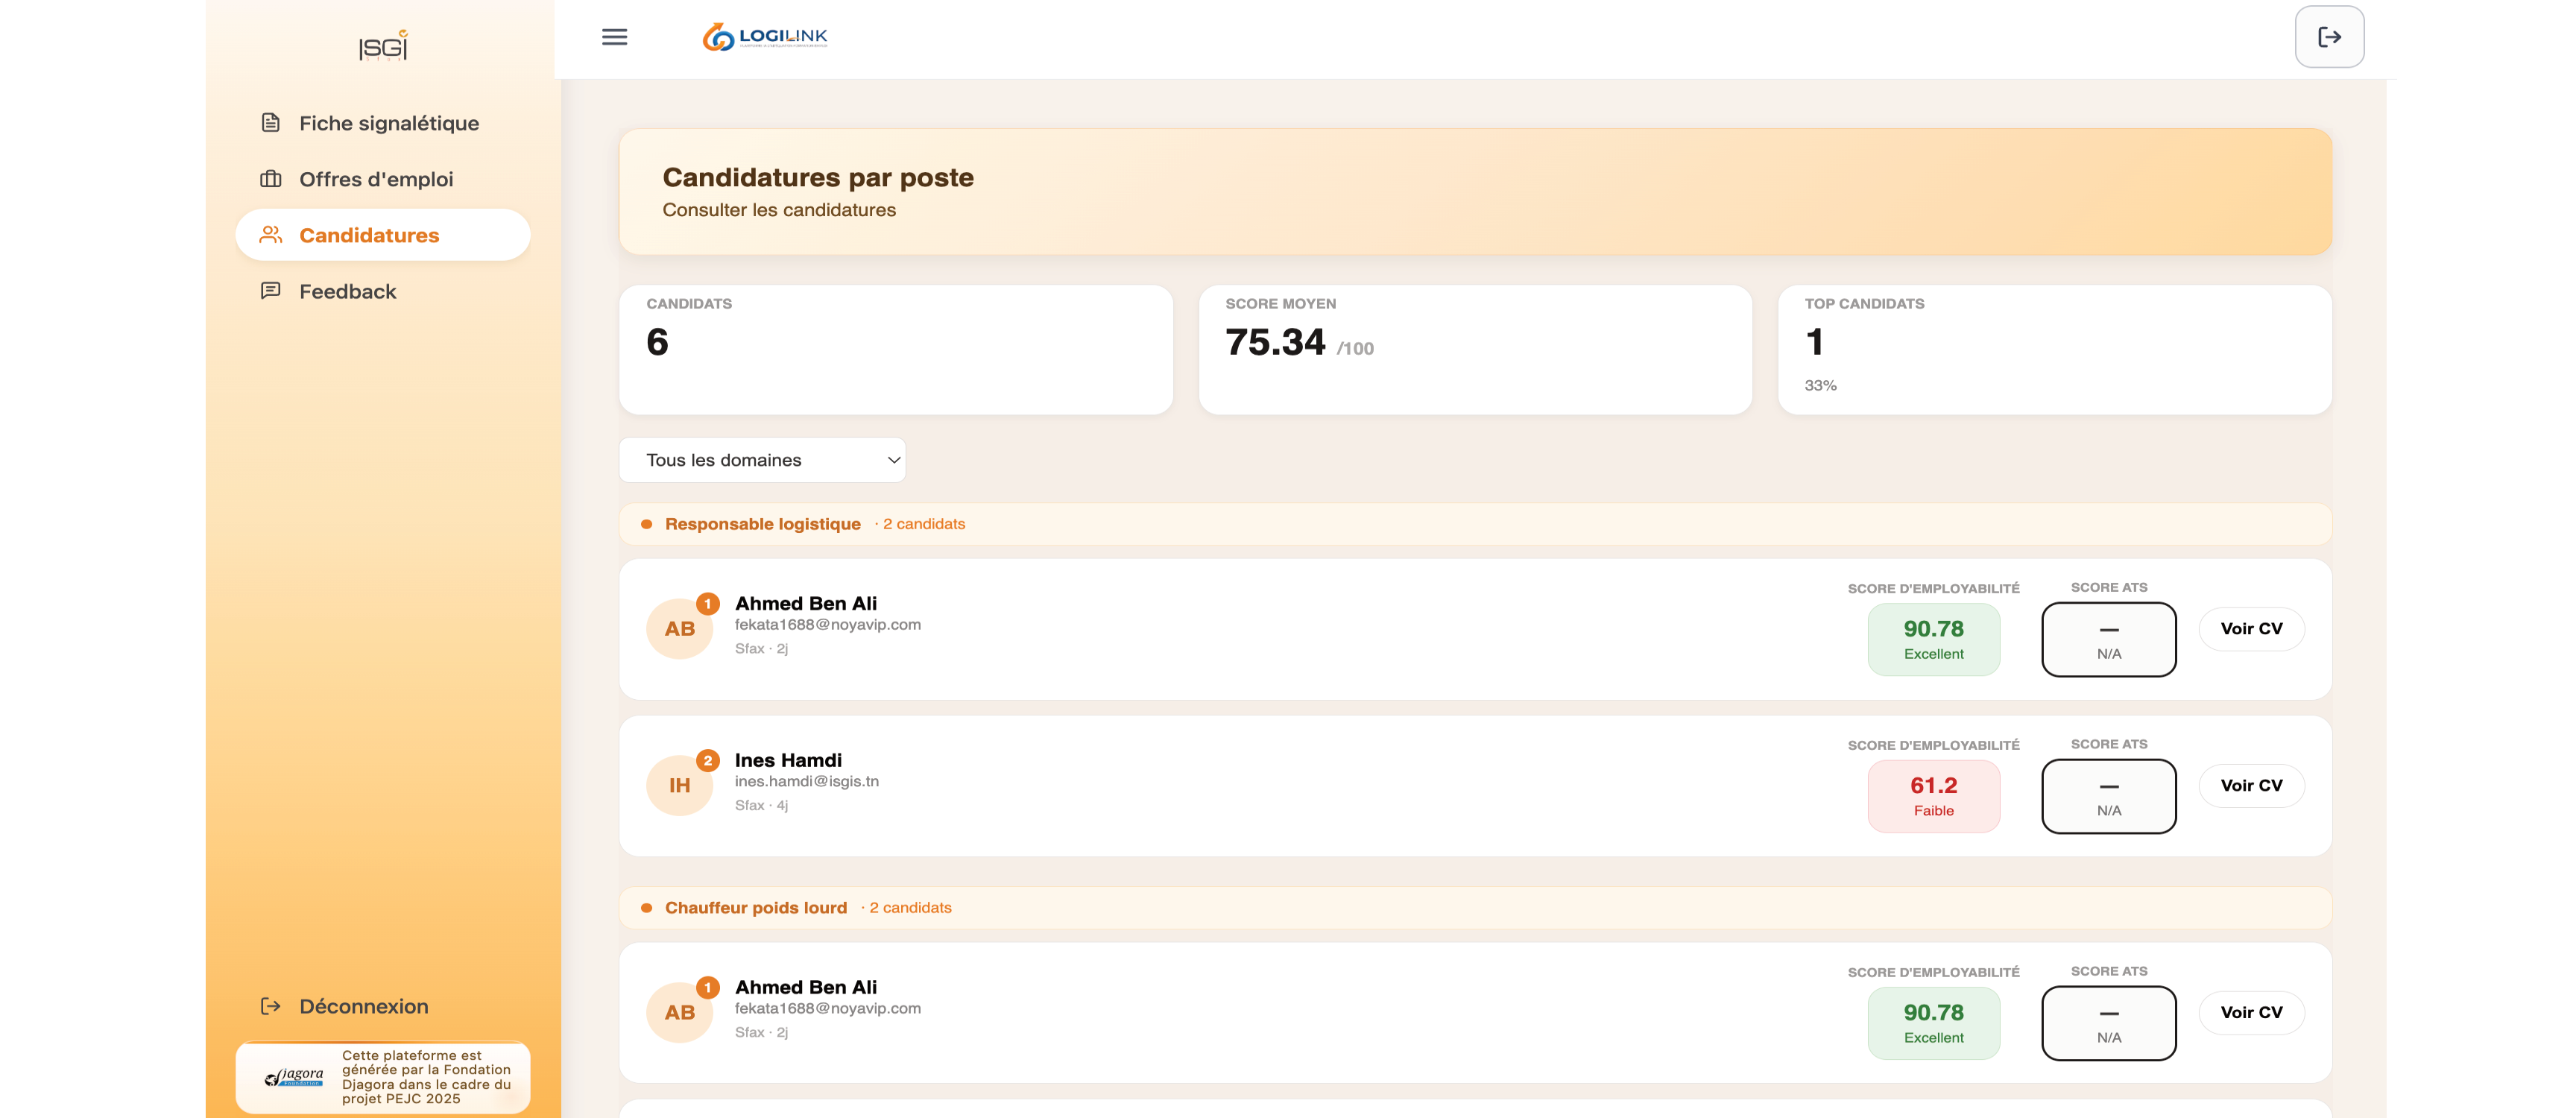
\includegraphics[width=0.85\textwidth]{figures/Interface_de_consultation_des_candidatures.png}
\caption{Interface de consultation des candidatures}
\label{fig:consultation-candidatures}
\end{figure}

\section{Conclusion}

Ce chapitre présente les environnements matériel et logiciel mis en place pour la réalisation du système, ainsi que les principales technologies adoptées pour son développement. L'environnement logiciel s'appuie sur des outils adaptés au travail collaboratif et au développement, tels que Visual Studio Code et GitHub, et sur un ensemble de technologies couvrant les différents besoins de la solution, par exemple Python pour le traitement et l'analyse des données, Node.js / NestJS pour la couche backend, Angular / TypeScript pour l'interface web, ainsi que MongoDB et Supabase (PostgreSQL) pour la gestion et le stockage des données.

\noindent Enfin, les interfaces développées ont permis de rendre le système accessible et facile à exploiter, en s'adaptant aux besoins de chaque profil (étudiant, administrateur et société). Elles proposent une navigation claire et des tableaux de bord facilitant la consultation des informations, tout en assurant une expérience utilisateur cohérente.


% ─────────────────────────────────────────────────────────────────────────────
% CONCLUSION GÉNÉRALE
% ─────────────────────────────────────────────────────────────────────────────
\chapter*{Conclusion Générale}
\addcontentsline{toc}{chapter}{Conclusion Générale}
\markboth{Conclusion Générale}{}

Ce projet de fin d'études a permis de mettre en pratique les connaissances acquises durant la formation académique dans un contexte entrepreneurial réel. Le travail a couvert l'étude des modèles économiques, l'analyse des métriques de performance, et la planification agile pour le développement de produits minimaux viables.

\vspace{12pt}

[Write your full general conclusion here]

\vspace{12pt}

\textbf{Perspectives :}
\begin{itemize}[leftmargin=*]
  \item [Perspective 1]
  \item [Perspective 2]
  \item [Perspective 3]
\end{itemize}

\newpage

% ─────────────────────────────────────────────────────────────────────────────
% BIBLIOGRAPHY
% ─────────────────────────────────────────────────────────────────────────────
\chapter*{Bibliographie}
\addcontentsline{toc}{chapter}{Bibliographie}

\begin{enumerate}
  \item Coursera for Campus, \url{https://www.coursera.org/campus}

  \item Forage, \url{https://www.theforage.com/}

  \item Jobscan, \url{https://www.jobscan.com/}

  \item 1Mentor, \url{https://www.1mentor.io/}

  \item Le modèle Waterfall, \url{https://www.techtarget.com/searchsoftwarequality/definition/waterfall-model}

  \item Le cycle en V, \url{https://improjet.fr/cycle-en-v-1/}

  \item Les méthodes agiles, \url{https://www.atlassian.com/agile}

  \item Scrum, \url{https://scrumguides.org/docs/scrumguide/v2020/2020-Scrum-Guide-US.pdf}

  \item Extreme Programming (XP), \url{https://www.techrepublic.com/article/what-is-extreme-programming/}

  \item DSDM (Dynamic Systems Development Method), \url{https://goodelearning.com/what-is-the-dynamic-systems-development-method-dsdm/}

  \item AFT Développement, \url{https://www.aft-dev.com/}
\end{enumerate}

\newpage

% ─────────────────────────────────────────────────────────────────────────────
% APPENDICES
% ─────────────────────────────────────────────────────────────────────────────
\appendix

% =============================================================================
% APPENDIX A — Supplementary Materials
% =============================================================================

\chapter{Documents Complémentaires}
\label{app:supplementary}

Ce chapitre contient les documents complémentaires référencés dans le corps du rapport.

\section{Cahier des Charges}
\label{sec:cahier-charges}

[Write your content here — requirements specification]

\section{Questionnaires et Sondages}
\label{sec:surveys}

[Write your content here — surveys conducted]

\section{Captures d'Écran Supplémentaires}
\label{sec:extra-screenshots}

[Insert additional screenshots here]

\begin{figure}[H]
  \centering
  % \includegraphics[width=0.9\textwidth]{figures/appendix-screenshot1}
  \rule{0.9\textwidth}{5cm} % placeholder
  \caption{Capture d'écran supplémentaire}
  \label{fig:appendix-screenshot1}
\end{figure}

% =============================================================================
% APPENDIX B — Technical Documentation
% =============================================================================

\chapter{Documentation Technique}
\label{app:technical}

Ce chapitre contient la documentation technique relative aux développements réalisés.

\section{Architecture Technique}
\label{sec:tech-architecture}

[Write your content here — system architecture, deployment diagrams]

\begin{figure}[H]
  \centering
  % \includegraphics[width=0.9\textwidth]{figures/architecture-diagram}
  \rule{0.9\textwidth}{5cm} % placeholder
  \caption{Architecture technique du système}
  \label{fig:architecture-diagram}
\end{figure}

\section{Diagrammes UML}
\label{sec:uml-diagrams}

[Write your content here — class diagrams, sequence diagrams, use case diagrams]

\section{Extraits de Code}
\label{sec:code-snippets}

[Write your content here — key code snippets]

\section{Guide d'Installation}
\label{sec:installation-guide}

[Write your content here — installation and setup instructions]


\end{document}
